\documentclass[a4paper]{book}
\usepackage{makeidx}
\usepackage{graphicx}
\usepackage{multicol}
\usepackage{float}
\usepackage{listings}
\usepackage{color}
\usepackage{ifthen}
\usepackage[table]{xcolor}
\usepackage{textcomp}
\usepackage{alltt}
\usepackage{ifpdf}
\ifpdf
\usepackage[pdftex,
            pagebackref=true,
            colorlinks=true,
            linkcolor=blue,
            unicode
           ]{hyperref}
\else
\usepackage[ps2pdf,
            pagebackref=true,
            colorlinks=true,
            linkcolor=blue,
            unicode
           ]{hyperref}
\usepackage{pspicture}
\fi
\usepackage[utf8]{inputenc}
\usepackage{mathptmx}
\usepackage[scaled=.90]{helvet}
\usepackage{courier}
\usepackage{sectsty}
\usepackage[titles]{tocloft}
\usepackage{doxygen}
\lstset{language=C++,inputencoding=utf8,basicstyle=\footnotesize,breaklines=true,breakatwhitespace=true,tabsize=8,numbers=left }
\makeindex
\setcounter{tocdepth}{3}
\renewcommand{\footrulewidth}{0.4pt}
\renewcommand{\familydefault}{\sfdefault}
\begin{document}
\hypersetup{pageanchor=false}
\begin{titlepage}
\vspace*{7cm}
\begin{center}
{\Large Reference Manual}\\
\vspace*{1cm}
{\large Generated by Doxygen 1.7.4}\\
\vspace*{0.5cm}
{\small Mon Aug 29 2011 19:00:31}\\
\end{center}
\end{titlepage}
\clearemptydoublepage
\pagenumbering{roman}
\tableofcontents
\clearemptydoublepage
\pagenumbering{arabic}
\hypersetup{pageanchor=true}
\chapter{GMU Earth Observation WCS v2.0 Documentation}
\label{index}\hypertarget{index}{}\hypertarget{index_intro}{}\section{Introduction}\label{index_intro}
This manual documents the C++ APIs for GMU EO-\/WCS.\par
 EO-\/WCS is an open source reference implementation for the Open Geospatial Consortium (OGC) Web Coverage Service (WCS) -\/ 8.\par
 ( For more information about EO-\/WCS, check the website: \href{http://geobrain.laits.gmu.edu/wcseodemo.html}{\tt http://geobrain.laits.gmu.edu/wcseodemo.html})\par
\hypertarget{index_license}{}\section{License}\label{index_license}
This software is released under the MIT license, anybody can use or modify the package, even for commercial applications.\par
 The only restriction is to retain the copyright in the sources or the binaries documentation.\par
 Neither the author, nor the university accept any responsibility for any kind of error or data loss which may occur during usage.\hypertarget{index_standards}{}\section{Followed Standards}\label{index_standards}

\begin{DoxyItemize}
\item OGC WCS 2.0 Interface Standard -\/ Core (OGC 09-\/110r3)
\item OGC WCS 2.0 Interface Standard -\/ \hyperlink{classKVP}{KVP} Protocol binding Extension (OGC 09-\/147r1)
\item OGC WCS 2.0 Interface Standard -\/ XML POST Protocol binding Extension (OGC 09-\/148r1)
\item OGC WCS 2.0 Application Profile -\/ Earth Observation (OGC 10-\/140)
\end{DoxyItemize}\hypertarget{index_reqlibs}{}\section{Required libraries}\label{index_reqlibs}

\begin{DoxyItemize}
\item GDAL library at server (\href{http://www.gdal.org}{\tt http://www.gdal.org})
\item HDF4 library at server (\href{http://www.hdfgroup.org}{\tt http://www.hdfgroup.org})
\item HDF5 library at server (\href{http://www.hdfgroup.org}{\tt http://www.hdfgroup.org})
\item HDF-\/EOS library at server (\href{http://www.hdfeos.org/}{\tt http://www.hdfeos.org/})
\end{DoxyItemize}

We tested this package with a Linux Fedora 12 and Mac OS 15 as the servers and clients.\hypertarget{index_supportformats}{}\section{Supported Data Type}\label{index_supportformats}

\begin{DoxyItemize}
\item HDF-\/EOS2 Grid, including MOD13C1, MOD09GQ, MYD15A2
\item HDF-\/EOS2 Swath, including MOD05\_\-L2
\item HDF-\/EOS5 Grid, including Aura OMSO2G
\item HDF-\/EOS5 Swath, including Aura OMDOAO3
\item HDF4, Tropical Rainfall Measuring Mission (TRMM)
\item NetCDF, NOAA GOES Imager data
\end{DoxyItemize}\hypertarget{index_compilenotes}{}\section{Compiling Notes}\label{index_compilenotes}
GDAL library is needed before compiling WCS package.\par
 Be sure that the support to HDF4 library should be enabled in GDAL library when compiling GDAL from source code.\par
 HDF-\/EOS library is also required to enable the HDF-\/EOS export format.\hypertarget{index_sourceCode}{}\section{Source Code}\label{index_sourceCode}
GMU WCS source code can be downloaded from \href{http://geobrain.laits.gmu.edu/ows8/code/gmu_eowcs_v0.1.tar.gz}{\tt http://geobrain.laits.gmu.edu/ows8/code/gmu\_\-eowcs\_\-v0.1.tar.gz}

\begin{DoxyAuthor}{Author}
Yuanzheng Shao $<$\href{mailto:yshao3@gmu.edu}{\tt yshao3@gmu.edu}$>$, Liping Di $<$\href{mailto:ldi@gmu.edu}{\tt ldi@gmu.edu}$>$ 
\end{DoxyAuthor}

\chapter{Todo List}
\label{todo}
\hypertarget{todo}{}
\label{todo__todo000001}
\hypertarget{todo__todo000001}{}
 
\begin{DoxyDescription}
\item[Member \hyperlink{classWCS__Configure_ae0fc8963b3530a687c0b6fca39e28519}{WCS\_\-Configure::Get\_\-STITCHED\_\-MOSAIC\_\-CONFIGRATION\_\-FILE\_\-PATH}() ]Currently (as of 07/22) the GMU WCS did not serve the data in the form of mosaic coverage, some demos will be added based on new requirement.
\end{DoxyDescription}

\label{todo__todo000002}
\hypertarget{todo__todo000002}{}
 
\begin{DoxyDescription}
\item[Member \hyperlink{classWCS__Configure_af82cfb1889f6ba7ce9a44dc644f2badc}{WCS\_\-Configure::Get\_\-TRANSACTION\_\-DATA\_\-DIRECTORY}() ]Currently (as of 07/22) the transaction interface of GMU WCS have not been tested.
\end{DoxyDescription}
\chapter{Class Index}
\section{Class Hierarchy}
This inheritance list is sorted roughly, but not completely, alphabetically:\begin{DoxyCompactList}
\item \contentsline{section}{AbstractDataset}{\pageref{classAbstractDataset}}{}
\begin{DoxyCompactList}
\item \contentsline{section}{HE4\_\-GRID\_\-Dataset}{\pageref{classHE4__GRID__Dataset}}{}
\item \contentsline{section}{HE4\_\-SWATH\_\-Dataset}{\pageref{classHE4__SWATH__Dataset}}{}
\item \contentsline{section}{HE5\_\-GRID\_\-Dataset}{\pageref{classHE5__GRID__Dataset}}{}
\item \contentsline{section}{HE5\_\-SWATH\_\-Dataset}{\pageref{classHE5__SWATH__Dataset}}{}
\item \contentsline{section}{NC\_\-GOES\_\-Dataset}{\pageref{classNC__GOES__Dataset}}{}
\item \contentsline{section}{TRMM\_\-Dataset}{\pageref{classTRMM__Dataset}}{}
\end{DoxyCompactList}
\item \contentsline{section}{BoundingBox}{\pageref{classBoundingBox}}{}
\item \contentsline{section}{CFGReader}{\pageref{classCFGReader}}{}
\item \contentsline{section}{DatasetObject}{\pageref{classDatasetObject}}{}
\item \contentsline{section}{DatasetSeriesObject}{\pageref{classDatasetSeriesObject}}{}
\item \contentsline{section}{KVP}{\pageref{classKVP}}{}
\item \contentsline{section}{KVPsReader}{\pageref{classKVPsReader}}{}
\item \contentsline{section}{My2DPoint}{\pageref{classMy2DPoint}}{}
\item \contentsline{section}{S2C}{\pageref{classS2C}}{}
\item \contentsline{section}{StitchedMosaicObject}{\pageref{classStitchedMosaicObject}}{}
\item \contentsline{section}{StringList}{\pageref{classStringList}}{}
\item \contentsline{section}{WCS\_\-Configure}{\pageref{classWCS__Configure}}{}
\item \contentsline{section}{WCS\_\-T}{\pageref{classWCS__T}}{}
\begin{DoxyCompactList}
\item \contentsline{section}{WCS\_\-DescribeCoverage}{\pageref{classWCS__DescribeCoverage}}{}
\item \contentsline{section}{WCS\_\-GetCapabilities}{\pageref{classWCS__GetCapabilities}}{}
\item \contentsline{section}{WCS\_\-GetCoverage}{\pageref{classWCS__GetCoverage}}{}
\end{DoxyCompactList}
\item \contentsline{section}{WCSCGI}{\pageref{classWCSCGI}}{}
\end{DoxyCompactList}

\chapter{Class Index}
\section{Class List}
Here are the classes, structs, unions and interfaces with brief descriptions:\begin{DoxyCompactList}
\item\contentsline{section}{\hyperlink{classAbstractDataset}{AbstractDataset} (Abstract dataset model definition. Based on GDAL dataset model )}{\pageref{classAbstractDataset}}{}
\item\contentsline{section}{\hyperlink{classBoundingBox}{BoundingBox} }{\pageref{classBoundingBox}}{}
\item\contentsline{section}{\hyperlink{classCFGReader}{CFGReader} }{\pageref{classCFGReader}}{}
\item\contentsline{section}{\hyperlink{classDatasetObject}{DatasetObject} (\hyperlink{classDatasetObject}{DatasetObject} class is used to record Dataset coverage attributes )}{\pageref{classDatasetObject}}{}
\item\contentsline{section}{\hyperlink{classDatasetSeriesObject}{DatasetSeriesObject} (\hyperlink{classDatasetSeriesObject}{DatasetSeriesObject} class is used to record dataset series coverage attributes )}{\pageref{classDatasetSeriesObject}}{}
\item\contentsline{section}{\hyperlink{classHE4__GRID__Dataset}{HE4\_\-GRID\_\-Dataset} (\hyperlink{classHE4__GRID__Dataset}{HE4\_\-GRID\_\-Dataset} is a subclass of \hyperlink{classAbstractDataset}{AbstractDataset}, used to process HDF-\/EOS2 Grid coverage )}{\pageref{classHE4__GRID__Dataset}}{}
\item\contentsline{section}{\hyperlink{classHE4__SWATH__Dataset}{HE4\_\-SWATH\_\-Dataset} (\hyperlink{classHE4__SWATH__Dataset}{HE4\_\-SWATH\_\-Dataset} is a subclass of \hyperlink{classAbstractDataset}{AbstractDataset}, used to process HDF-\/EOS2 Swath coverage )}{\pageref{classHE4__SWATH__Dataset}}{}
\item\contentsline{section}{\hyperlink{classHE5__GRID__Dataset}{HE5\_\-GRID\_\-Dataset} (\hyperlink{classHE5__GRID__Dataset}{HE5\_\-GRID\_\-Dataset} is a subclass of \hyperlink{classAbstractDataset}{AbstractDataset}, used to process HDF-\/EOS5 Grid coverage )}{\pageref{classHE5__GRID__Dataset}}{}
\item\contentsline{section}{\hyperlink{classHE5__SWATH__Dataset}{HE5\_\-SWATH\_\-Dataset} (\hyperlink{classHE5__SWATH__Dataset}{HE5\_\-SWATH\_\-Dataset} is a subclass of \hyperlink{classAbstractDataset}{AbstractDataset}, used to process HDF-\/EOS5 Swath coverage )}{\pageref{classHE5__SWATH__Dataset}}{}
\item\contentsline{section}{\hyperlink{classKVP}{KVP} }{\pageref{classKVP}}{}
\item\contentsline{section}{\hyperlink{classKVPsReader}{KVPsReader} }{\pageref{classKVPsReader}}{}
\item\contentsline{section}{\hyperlink{classMy2DPoint}{My2DPoint} }{\pageref{classMy2DPoint}}{}
\item\contentsline{section}{\hyperlink{classNC__GOES__Dataset}{NC\_\-GOES\_\-Dataset} (\hyperlink{classNC__GOES__Dataset}{NC\_\-GOES\_\-Dataset} is a subclass of \hyperlink{classAbstractDataset}{AbstractDataset}, used to process NOAA GOES data )}{\pageref{classNC__GOES__Dataset}}{}
\item\contentsline{section}{\hyperlink{classS2C}{S2C} }{\pageref{classS2C}}{}
\item\contentsline{section}{\hyperlink{classStitchedMosaicObject}{StitchedMosaicObject} (\hyperlink{classStitchedMosaicObject}{StitchedMosaicObject} class is used to record stitched mosaic coverage attributes )}{\pageref{classStitchedMosaicObject}}{}
\item\contentsline{section}{\hyperlink{classStringList}{StringList} }{\pageref{classStringList}}{}
\item\contentsline{section}{\hyperlink{classTRMM__Dataset}{TRMM\_\-Dataset} (\hyperlink{classTRMM__Dataset}{TRMM\_\-Dataset} is a subclass of \hyperlink{classAbstractDataset}{AbstractDataset}, used to process TRMM coverage )}{\pageref{classTRMM__Dataset}}{}
\item\contentsline{section}{\hyperlink{classWCS__Configure}{WCS\_\-Configure} (Configuration class provides fetch methods to get information from WCS configuration file )}{\pageref{classWCS__Configure}}{}
\item\contentsline{section}{\hyperlink{classWCS__DescribeCoverage}{WCS\_\-DescribeCoverage} (This class is used to handle DescribeCoverage and DescribeEOCoverageSet request )}{\pageref{classWCS__DescribeCoverage}}{}
\item\contentsline{section}{\hyperlink{classWCS__GetCapabilities}{WCS\_\-GetCapabilities} (This class is used to handle GetCapabilities request )}{\pageref{classWCS__GetCapabilities}}{}
\item\contentsline{section}{\hyperlink{classWCS__GetCoverage}{WCS\_\-GetCoverage} (This class is used to handle GetCoverage request )}{\pageref{classWCS__GetCoverage}}{}
\item\contentsline{section}{\hyperlink{classWCS__T}{WCS\_\-T} (\hyperlink{classWCS__T}{WCS\_\-T} is a upper class for handling WCS request )}{\pageref{classWCS__T}}{}
\item\contentsline{section}{\hyperlink{classWCSCGI}{WCSCGI} }{\pageref{classWCSCGI}}{}
\end{DoxyCompactList}

\chapter{Class Documentation}
\hypertarget{classAbstractDataset}{
\section{AbstractDataset Class Reference}
\label{classAbstractDataset}\index{AbstractDataset@{AbstractDataset}}
}


Abstract dataset model definition. Based on GDAL dataset model.  




{\ttfamily \#include $<$AbstractDataset.h$>$}

Inheritance diagram for AbstractDataset:\begin{figure}[H]
\begin{center}
\leavevmode
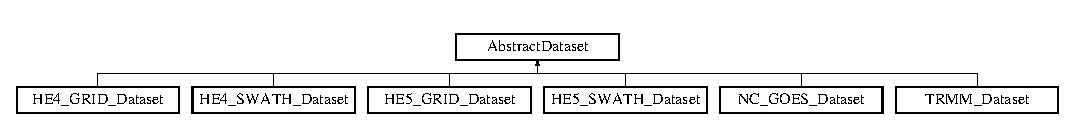
\includegraphics[height=1.296296cm]{classAbstractDataset}
\end{center}
\end{figure}
\subsection*{Public Member Functions}
\begin{DoxyCompactItemize}
\item 
\hyperlink{classAbstractDataset_ad00421fe0b425cdbc26c68c5dc724bee}{AbstractDataset} (const string \&, vector$<$ int $>$ \&)
\begin{DoxyCompactList}\small\item\em Constructor of an \hyperlink{classAbstractDataset}{AbstractDataset}. \end{DoxyCompactList}\item 
virtual \hyperlink{classAbstractDataset_a144cd670169b00b62afbdc2ded2639fa}{$\sim$AbstractDataset} ()
\begin{DoxyCompactList}\small\item\em Destroy an open \hyperlink{classAbstractDataset}{AbstractDataset} object. \end{DoxyCompactList}\item 
GDALDataset $\ast$ \hyperlink{classAbstractDataset_aed8db0cfc46d0171f692364bbf1a7dcf}{GetGDALDataset} ()
\begin{DoxyCompactList}\small\item\em Get the GDALDataset object from AbstarctDataset. \end{DoxyCompactList}\item 
virtual CPLErr \hyperlink{classAbstractDataset_a45924895c6bf26c7f75d503b8f6e388a}{InitialDataset} (const int isSimple=0)
\begin{DoxyCompactList}\small\item\em Initialize the data set. \end{DoxyCompactList}\item 
const OGRSpatialReference \& \hyperlink{classAbstractDataset_a4d92be8700505a6a7ef6655e35b05725}{GetNativeCRS} ()
\begin{DoxyCompactList}\small\item\em Get the Native CRS of an AbstarctDataset. \end{DoxyCompactList}\item 
const double \& \hyperlink{classAbstractDataset_aada8065023ba9b718c0d759698365b40}{GetMissingValue} ()
\begin{DoxyCompactList}\small\item\em Fetch the filled value (missing value) of a coverage. \end{DoxyCompactList}\item 
int \hyperlink{classAbstractDataset_adbf83ce500a0f30b79ca682df26638e4}{GetGeoTransform} (double geoTrans\mbox{[}$\,$\mbox{]})
\begin{DoxyCompactList}\small\item\em Fetch the affine transformation coefficients. \end{DoxyCompactList}\item 
vector$<$ string $>$ \hyperlink{classAbstractDataset_a736080454f7ac794c710f00da26e37f9}{GetMetaDataList} ()
\begin{DoxyCompactList}\small\item\em Fetch the metadata list for this coverage. \end{DoxyCompactList}\item 
vector$<$ int $>$ \hyperlink{classAbstractDataset_a83b521f96ef4b5fe5b5062707ecc7f40}{GetBandList} ()
\begin{DoxyCompactList}\small\item\em Fetch the contained band list of request coverage. \end{DoxyCompactList}\item 
void \hyperlink{classAbstractDataset_a919760d8e60c26b105740bc2bc109b0e}{GetNativeBBox} (double bBox\mbox{[}$\,$\mbox{]})
\begin{DoxyCompactList}\small\item\em Fetch the bounding box of a coverage under the native CRS. \end{DoxyCompactList}\item 
CPLErr \hyperlink{classAbstractDataset_a66a65ce60f813d0ef683919a098b8a98}{GetGeoMinMax} (double geoMinMax\mbox{[}$\,$\mbox{]})
\begin{DoxyCompactList}\small\item\em Fetch the bounding box of a coverage under EPSG:4326. \end{DoxyCompactList}\item 
int \hyperlink{classAbstractDataset_a83c0bc843f701e8b20b5408b9c7e0731}{GetImageBandCount} ()
\begin{DoxyCompactList}\small\item\em Fetch the number of raster bands on this dataset. \end{DoxyCompactList}\item 
int \hyperlink{classAbstractDataset_a950e120c5a1e9fa06ee5b02ed4fc6c42}{GetImageXSize} ()
\begin{DoxyCompactList}\small\item\em Fetch coverage width in pixels. \end{DoxyCompactList}\item 
int \hyperlink{classAbstractDataset_a4f7ceb09ad968d28a5282c7652fb6975}{GetImageYSize} ()
\begin{DoxyCompactList}\small\item\em Fetch coverage height in pixels. \end{DoxyCompactList}\item 
string \hyperlink{classAbstractDataset_ab7b76c03b2a94853b631b83ebb1be453}{GetResourceFileName} ()
\begin{DoxyCompactList}\small\item\em Fetch the resource file name of a coverage. \end{DoxyCompactList}\item 
string \hyperlink{classAbstractDataset_a93b5fa34e8ace1dd9c30abad1f3e2f72}{GetDatasetName} ()
\begin{DoxyCompactList}\small\item\em Fetch the dataset name of a coverage. \end{DoxyCompactList}\item 
string \hyperlink{classAbstractDataset_a5a6c03e8c1f796ef1ffd018016b342fa}{GetDataTypeName} ()
\begin{DoxyCompactList}\small\item\em Fetch the dataset type name of a coverage. \end{DoxyCompactList}\item 
string \hyperlink{classAbstractDataset_a9c37d346022864bf92f5d9d33e45fd42}{GetNativeFormat} ()
\begin{DoxyCompactList}\small\item\em Fetch the native format of a coverage. \end{DoxyCompactList}\item 
string \hyperlink{classAbstractDataset_a6d91e0d5d812e4a9b796796cb8fc45a3}{GetCoverageID} ()
\begin{DoxyCompactList}\small\item\em Fetch the identifier of a coverage. \end{DoxyCompactList}\item 
string \hyperlink{classAbstractDataset_ace176d7bf4a12ae58e48ded2da210a86}{GetDatasetDescription} ()
\begin{DoxyCompactList}\small\item\em Fetch the dataset description of a coverage. \end{DoxyCompactList}\item 
string \hyperlink{classAbstractDataset_ab4509cea5f99f8ebeb836d85828c3470}{GetNativeCRS\_\-URN} ()
\begin{DoxyCompactList}\small\item\em Fetch the native CRS code of coverage. \end{DoxyCompactList}\item 
string \hyperlink{classAbstractDataset_a8172c4de7f03007cd17a54149c801627}{GetGeoCRS\_\-URN} ()
\begin{DoxyCompactList}\small\item\em Fetch the Geographic CRS code of coverage. \end{DoxyCompactList}\item 
string \hyperlink{classAbstractDataset_a2e6cdb6c0d165543a8a4d936835db73b}{GetProjectionRef} ()
\begin{DoxyCompactList}\small\item\em Fetch the native projection reference of a coverage. \end{DoxyCompactList}\item 
string \hyperlink{classAbstractDataset_a90a2e56cacec8d9aa13b6fb66a862bf6}{GetCoverageBeginTime} ()
\begin{DoxyCompactList}\small\item\em Fetch the begin date/time of a coverage. \end{DoxyCompactList}\item 
string \hyperlink{classAbstractDataset_a8193da35dd2e264834ac3af2bd89a0c0}{GetCoverageEndTime} ()
\begin{DoxyCompactList}\small\item\em Fetch the end date/time of a coverage. \end{DoxyCompactList}\item 
string \hyperlink{classAbstractDataset_a505f9a6143ef694db5c7ff324f5c891a}{GetCoverageSubType} ()
\begin{DoxyCompactList}\small\item\em Fetch the coverage type. \end{DoxyCompactList}\item 
string \hyperlink{classAbstractDataset_a641d024862d22d4b8598ffa3dd5ef43e}{GetFieldQuantityDef} ()
\begin{DoxyCompactList}\small\item\em Fetch the field units of a coverage. \end{DoxyCompactList}\item 
string \hyperlink{classAbstractDataset_aa4e7985dc41a9eb44254bbc9782e6b1d}{GetAllowValues} ()
\begin{DoxyCompactList}\small\item\em Fetch the allow values of a coverage. \end{DoxyCompactList}\item 
string \hyperlink{classAbstractDataset_a6dab64e60c0cd4799408caf7afffb1cb}{GetISO19115Metadata} ()
\begin{DoxyCompactList}\small\item\em Fetch the coverage metadata which is compliant to ISO 19115:2003. \end{DoxyCompactList}\item 
string \hyperlink{classAbstractDataset_a25e49f67a2e5e84465d2b32a8b2457cb}{GetCoverageArchiveTime} ()
\begin{DoxyCompactList}\small\item\em Fetch the archive date/time of this dataset. \end{DoxyCompactList}\item 
string \hyperlink{classAbstractDataset_af98c41e04bc2f1f6ca57cf88b7dc34c4}{GetCoveragePlatform} ()
\begin{DoxyCompactList}\small\item\em Fetch the platform name of this dataset. \end{DoxyCompactList}\item 
string \hyperlink{classAbstractDataset_a258a7f882e62f899fe1ceb75fa8849f9}{GetCoverageInstrument} ()
\begin{DoxyCompactList}\small\item\em Fetch the instrument name of this dataset. \end{DoxyCompactList}\item 
string \hyperlink{classAbstractDataset_a9a60a3d1b5b094c58bbc927a58f22e6d}{GetCoverageSensor} ()
\begin{DoxyCompactList}\small\item\em Fetch the sensor name of this dataset. \end{DoxyCompactList}\item 
int \hyperlink{classAbstractDataset_a206bf47490d90bd0698fe2c491106c84}{IsbGeoTransformSet} ()
\begin{DoxyCompactList}\small\item\em Determine whether set the affine geoTransform for a coverage. \end{DoxyCompactList}\item 
int \hyperlink{classAbstractDataset_a3597ba14546a8fd5b0ea0bad7f9583e0}{IsCrossingIDL} ()
\begin{DoxyCompactList}\small\item\em Determine whether the extend of coverage cross the International Date Line (IDL). \end{DoxyCompactList}\item 
CPLErr \hyperlink{classAbstractDataset_a339c58a6e439d0877d8b09e1d2d26b31}{GetSuggestedWarpResolution} (OGRSpatialReference \&dstCRS, double adfDstGeoTransform\mbox{[}$\,$\mbox{]}, int \&nPixels, int \&nLines)
\begin{DoxyCompactList}\small\item\em Get the suggested warp option, method 1. \end{DoxyCompactList}\item 
CPLErr \hyperlink{classAbstractDataset_aed58e61df99fd00c205fafef519639ee}{GetSuggestedWarpResolution2} (OGRSpatialReference \&dstCRS, double adfDstGeoTransform\mbox{[}$\,$\mbox{]}, int \&nPixels, int \&nLines)
\begin{DoxyCompactList}\small\item\em Get the suggested warp option, method 2. \end{DoxyCompactList}\item 
GDALDataset $\ast$ \hyperlink{classAbstractDataset_a55257132908f4fa578f44b1bb485dcaa}{DatasetWarper} (int \&IsRefDS, OGRSpatialReference \&dstCRS, int \&iDstRasterXsize, int \&iDstRasterYsize, double pDstGeoTransform\mbox{[}$\,$\mbox{]}, GDALResampleAlg eResampleAlg=GRA\_\-NearestNeighbour)
\begin{DoxyCompactList}\small\item\em Wrap the dataset to a GDALDataset object based on input parameters. \end{DoxyCompactList}\end{DoxyCompactItemize}
\subsection*{Protected Member Functions}
\begin{DoxyCompactItemize}
\item 
virtual CPLErr \hyperlink{classAbstractDataset_acfac922d16e5edf51066169bd6ff28ec}{SetNativeCRS} ()
\begin{DoxyCompactList}\small\item\em Set the Native CRS for an AbstarctDataset. \end{DoxyCompactList}\item 
virtual CPLErr \hyperlink{classAbstractDataset_a1d79fc347de75acd57b18c80b9614369}{SetGeoTransform} ()
\begin{DoxyCompactList}\small\item\em Set the affine GeoTransform matrix for a coverage. \end{DoxyCompactList}\item 
virtual CPLErr \hyperlink{classAbstractDataset_a93bd80bfa48ad45ea53599f289406287}{SetGDALDataset} (const int isSimple=0)
\begin{DoxyCompactList}\small\item\em Set the GDALDataset object to AbstarctDataset. \end{DoxyCompactList}\item 
virtual CPLErr \hyperlink{classAbstractDataset_af3f0b55b14f660b79751bf88489a2c10}{SetMetaDataList} (GDALDataset $\ast$)
\begin{DoxyCompactList}\small\item\em Set the metadata list for this coverage based on dataset object. \end{DoxyCompactList}\end{DoxyCompactItemize}
\subsection*{Protected Attributes}
\begin{DoxyCompactItemize}
\item 
\hypertarget{classAbstractDataset_a0a7aa031c18bc61b12eb8e23a0852ade}{
auto\_\-ptr$<$ GDALDataset $>$ {\bfseries maptrDS}}
\label{classAbstractDataset_a0a7aa031c18bc61b12eb8e23a0852ade}

\item 
\hypertarget{classAbstractDataset_ad241c44de1a16de00a88195bb3b08deb}{
string {\bfseries ms\_\-CoverageID}}
\label{classAbstractDataset_ad241c44de1a16de00a88195bb3b08deb}

\item 
\hypertarget{classAbstractDataset_a5f3f63f66c91ce61213ae966ed0a593b}{
string {\bfseries ms\_\-CoverageBeginTime}}
\label{classAbstractDataset_a5f3f63f66c91ce61213ae966ed0a593b}

\item 
\hypertarget{classAbstractDataset_a2bf942bae502e9b9a02ee8b5cc4d4fb7}{
string {\bfseries ms\_\-CoverageEndTime}}
\label{classAbstractDataset_a2bf942bae502e9b9a02ee8b5cc4d4fb7}

\item 
\hypertarget{classAbstractDataset_ac8fd3b9fb9f9e1d8921e2cde2c75ecaf}{
string {\bfseries ms\_\-CoverageSubType}}
\label{classAbstractDataset_ac8fd3b9fb9f9e1d8921e2cde2c75ecaf}

\item 
\hypertarget{classAbstractDataset_a603719678668fef176a65bd33d426d0b}{
string {\bfseries ms\_\-CoverageArchiveTime}}
\label{classAbstractDataset_a603719678668fef176a65bd33d426d0b}

\item 
\hypertarget{classAbstractDataset_ad7f7925c2866e662f75ff10364d01ba6}{
string {\bfseries ms\_\-CoveragePlatform}}
\label{classAbstractDataset_ad7f7925c2866e662f75ff10364d01ba6}

\item 
\hypertarget{classAbstractDataset_afe2f6a655cd353db5c0e111ef2690edf}{
string {\bfseries ms\_\-CoverageInstrument}}
\label{classAbstractDataset_afe2f6a655cd353db5c0e111ef2690edf}

\item 
\hypertarget{classAbstractDataset_a23ea7b2d8b63056c481ec42014db4c4c}{
string {\bfseries ms\_\-CoverageSensor}}
\label{classAbstractDataset_a23ea7b2d8b63056c481ec42014db4c4c}

\item 
\hypertarget{classAbstractDataset_ad432bb31a7c73f5ccfa5e38c59cee950}{
string {\bfseries ms\_\-SrcFilename}}
\label{classAbstractDataset_ad432bb31a7c73f5ccfa5e38c59cee950}

\item 
\hypertarget{classAbstractDataset_afd00d5bdfa29b266b71d54e543b0d31f}{
string {\bfseries ms\_\-DatasetName}}
\label{classAbstractDataset_afd00d5bdfa29b266b71d54e543b0d31f}

\item 
\hypertarget{classAbstractDataset_ad226ee89e3bc3264a1443b5fa38bc49c}{
string {\bfseries ms\_\-DataTypeName}}
\label{classAbstractDataset_ad226ee89e3bc3264a1443b5fa38bc49c}

\item 
\hypertarget{classAbstractDataset_ac003715ef548373ed0504bb5383cf03b}{
string {\bfseries ms\_\-NativeFormat}}
\label{classAbstractDataset_ac003715ef548373ed0504bb5383cf03b}

\item 
\hypertarget{classAbstractDataset_ab0c3eac75d38db6ba50d0bc43361eac2}{
string {\bfseries ms\_\-FieldQuantityDef}}
\label{classAbstractDataset_ab0c3eac75d38db6ba50d0bc43361eac2}

\item 
\hypertarget{classAbstractDataset_af56c63636750a88521d6da9ed1225495}{
string {\bfseries ms\_\-AllowRanges}}
\label{classAbstractDataset_af56c63636750a88521d6da9ed1225495}

\item 
\hypertarget{classAbstractDataset_ac3ae79d84fdf4e0058091b47be0b2f10}{
string {\bfseries ms\_\-ISO19115Metadata}}
\label{classAbstractDataset_ac3ae79d84fdf4e0058091b47be0b2f10}

\item 
\hypertarget{classAbstractDataset_a2769492120ab8786156dc008f4df66ba}{
vector$<$ int $>$ {\bfseries mv\_\-BandList}}
\label{classAbstractDataset_a2769492120ab8786156dc008f4df66ba}

\item 
\hypertarget{classAbstractDataset_a305de13cdca7f2333a22c7128e6636df}{
vector$<$ string $>$ {\bfseries mv\_\-MeteDataList}}
\label{classAbstractDataset_a305de13cdca7f2333a22c7128e6636df}

\item 
\hypertarget{classAbstractDataset_abb20036310c1fe91a9f32ff52c4f0418}{
double {\bfseries md\_\-Geotransform} \mbox{[}6\mbox{]}}
\label{classAbstractDataset_abb20036310c1fe91a9f32ff52c4f0418}

\item 
\hypertarget{classAbstractDataset_a34ebf17165933f54cf1e556ae7aa7ed3}{
double {\bfseries md\_\-GeoMinMax} \mbox{[}4\mbox{]}}
\label{classAbstractDataset_a34ebf17165933f54cf1e556ae7aa7ed3}

\item 
\hypertarget{classAbstractDataset_a4ff76800a2f8e561fc5aa86d536c396c}{
double {\bfseries md\_\-MissingValue}}
\label{classAbstractDataset_a4ff76800a2f8e561fc5aa86d536c396c}

\item 
\hypertarget{classAbstractDataset_a4bb09d130d94e550ece8145f1e5498e0}{
int {\bfseries mb\_\-GeoTransformSet}}
\label{classAbstractDataset_a4bb09d130d94e550ece8145f1e5498e0}

\item 
\hypertarget{classAbstractDataset_a7233ac7625660c30f9b82e4aa61701cb}{
int {\bfseries mb\_\-IsVirtualDS}}
\label{classAbstractDataset_a7233ac7625660c30f9b82e4aa61701cb}

\item 
\hypertarget{classAbstractDataset_abac7fcd9967f805f3cc81053f9c6576e}{
OGRSpatialReference {\bfseries mo\_\-NativeCRS}}
\label{classAbstractDataset_abac7fcd9967f805f3cc81053f9c6576e}

\end{DoxyCompactItemize}


\subsection{Detailed Description}
Abstract dataset model definition. Based on GDAL dataset model. 

An abstract dataset encapsulating one or more raster bands, which is based on GDALDataset, and add the support to metadata model: ISO 19115 and 1SO 19115 (2). A series of Fetch functions are provided for the implementation of Web Coverage Service.

Use WCSTCreateDataset() to create a \hyperlink{classAbstractDataset}{AbstractDataset} for a named coverage identifier and band list. 

\subsection{Constructor \& Destructor Documentation}
\hypertarget{classAbstractDataset_ad00421fe0b425cdbc26c68c5dc724bee}{
\index{AbstractDataset@{AbstractDataset}!AbstractDataset@{AbstractDataset}}
\index{AbstractDataset@{AbstractDataset}!AbstractDataset@{AbstractDataset}}
\subsubsection[{AbstractDataset}]{\setlength{\rightskip}{0pt plus 5cm}AbstractDataset::AbstractDataset (
\begin{DoxyParamCaption}
\item[{const string \&}]{id, }
\item[{vector$<$ int $>$ \&}]{rBandList}
\end{DoxyParamCaption}
)}}
\label{classAbstractDataset_ad00421fe0b425cdbc26c68c5dc724bee}


Constructor of an \hyperlink{classAbstractDataset}{AbstractDataset}. 

This is the accepted method of opening an abstract dataset and allocating all resources associated with it. \hypertarget{classAbstractDataset_a144cd670169b00b62afbdc2ded2639fa}{
\index{AbstractDataset@{AbstractDataset}!$\sim$AbstractDataset@{$\sim$AbstractDataset}}
\index{$\sim$AbstractDataset@{$\sim$AbstractDataset}!AbstractDataset@{AbstractDataset}}
\subsubsection[{$\sim$AbstractDataset}]{\setlength{\rightskip}{0pt plus 5cm}AbstractDataset::$\sim$AbstractDataset (
\begin{DoxyParamCaption}
{}
\end{DoxyParamCaption}
)\hspace{0.3cm}{\ttfamily  \mbox{[}virtual\mbox{]}}}}
\label{classAbstractDataset_a144cd670169b00b62afbdc2ded2639fa}


Destroy an open \hyperlink{classAbstractDataset}{AbstractDataset} object. 

This is the accepted method of closing a \hyperlink{classAbstractDataset}{AbstractDataset} dataset and deallocating all resources associated with it. 

\subsection{Member Function Documentation}
\hypertarget{classAbstractDataset_a55257132908f4fa578f44b1bb485dcaa}{
\index{AbstractDataset@{AbstractDataset}!DatasetWarper@{DatasetWarper}}
\index{DatasetWarper@{DatasetWarper}!AbstractDataset@{AbstractDataset}}
\subsubsection[{DatasetWarper}]{\setlength{\rightskip}{0pt plus 5cm}GDALDataset $\ast$ AbstractDataset::DatasetWarper (
\begin{DoxyParamCaption}
\item[{int \&}]{IsRefDS, }
\item[{OGRSpatialReference \&}]{dstCRS, }
\item[{int \&}]{iDstRasterXsize, }
\item[{int \&}]{iDstRasterYsize, }
\item[{double}]{pDstGeoTransform\mbox{[}$\,$\mbox{]}, }
\item[{GDALResampleAlg}]{eResampleAlg = {\ttfamily GRA\_\-NearestNeighbour}}
\end{DoxyParamCaption}
)}}
\label{classAbstractDataset_a55257132908f4fa578f44b1bb485dcaa}


Wrap the dataset to a GDALDataset object based on input parameters. 

Wrap the dataset to a GDALDataset object based on input parameters.

\begin{DoxyReturn}{Returns}
the warpped GDALDataset object. 

GDALDatset object. 
\end{DoxyReturn}
\hypertarget{classAbstractDataset_aa4e7985dc41a9eb44254bbc9782e6b1d}{
\index{AbstractDataset@{AbstractDataset}!GetAllowValues@{GetAllowValues}}
\index{GetAllowValues@{GetAllowValues}!AbstractDataset@{AbstractDataset}}
\subsubsection[{GetAllowValues}]{\setlength{\rightskip}{0pt plus 5cm}string AbstractDataset::GetAllowValues (
\begin{DoxyParamCaption}
{}
\end{DoxyParamCaption}
)}}
\label{classAbstractDataset_aa4e7985dc41a9eb44254bbc9782e6b1d}


Fetch the allow values of a coverage. 

The method will return the valid range of a coverage. For example to MOD09GQ(collection name) sur\_\-refl\_\-b01\_\-1(dataset name) data, valid\_\-range equals to (-\/100, 16000).

\begin{DoxyReturn}{Returns}
the string of valid range of a coverage, in the forms of \char`\"{}min, max\char`\"{}. 
\end{DoxyReturn}
\hypertarget{classAbstractDataset_a83b521f96ef4b5fe5b5062707ecc7f40}{
\index{AbstractDataset@{AbstractDataset}!GetBandList@{GetBandList}}
\index{GetBandList@{GetBandList}!AbstractDataset@{AbstractDataset}}
\subsubsection[{GetBandList}]{\setlength{\rightskip}{0pt plus 5cm}vector$<$ int $>$ AbstractDataset::GetBandList (
\begin{DoxyParamCaption}
{}
\end{DoxyParamCaption}
)}}
\label{classAbstractDataset_a83b521f96ef4b5fe5b5062707ecc7f40}


Fetch the contained band list of request coverage. 

The method will return the contained band list of request coverage.

\begin{DoxyReturn}{Returns}
the band array. 
\end{DoxyReturn}
\hypertarget{classAbstractDataset_a25e49f67a2e5e84465d2b32a8b2457cb}{
\index{AbstractDataset@{AbstractDataset}!GetCoverageArchiveTime@{GetCoverageArchiveTime}}
\index{GetCoverageArchiveTime@{GetCoverageArchiveTime}!AbstractDataset@{AbstractDataset}}
\subsubsection[{GetCoverageArchiveTime}]{\setlength{\rightskip}{0pt plus 5cm}string AbstractDataset::GetCoverageArchiveTime (
\begin{DoxyParamCaption}
{}
\end{DoxyParamCaption}
)}}
\label{classAbstractDataset_a25e49f67a2e5e84465d2b32a8b2457cb}


Fetch the archive date/time of this dataset. 

The method will return the archive date/time of dataset (granule).

\begin{DoxyReturn}{Returns}
The string of archive date/time. 
\end{DoxyReturn}
\hypertarget{classAbstractDataset_a90a2e56cacec8d9aa13b6fb66a862bf6}{
\index{AbstractDataset@{AbstractDataset}!GetCoverageBeginTime@{GetCoverageBeginTime}}
\index{GetCoverageBeginTime@{GetCoverageBeginTime}!AbstractDataset@{AbstractDataset}}
\subsubsection[{GetCoverageBeginTime}]{\setlength{\rightskip}{0pt plus 5cm}string AbstractDataset::GetCoverageBeginTime (
\begin{DoxyParamCaption}
{}
\end{DoxyParamCaption}
)}}
\label{classAbstractDataset_a90a2e56cacec8d9aa13b6fb66a862bf6}


Fetch the begin date/time of a coverage. 

The method will return the begin date/time of a coverage. For MODIS data, each granule will cover a range of time; for TRMM data, the daily data will cover a whole day, and monthly data will cover a whole month.

\begin{DoxyReturn}{Returns}
the string of begin date/time corresponding to the coverage. 
\end{DoxyReturn}
\hypertarget{classAbstractDataset_a8193da35dd2e264834ac3af2bd89a0c0}{
\index{AbstractDataset@{AbstractDataset}!GetCoverageEndTime@{GetCoverageEndTime}}
\index{GetCoverageEndTime@{GetCoverageEndTime}!AbstractDataset@{AbstractDataset}}
\subsubsection[{GetCoverageEndTime}]{\setlength{\rightskip}{0pt plus 5cm}string AbstractDataset::GetCoverageEndTime (
\begin{DoxyParamCaption}
{}
\end{DoxyParamCaption}
)}}
\label{classAbstractDataset_a8193da35dd2e264834ac3af2bd89a0c0}


Fetch the end date/time of a coverage. 

The method will return the end date/time of a coverage. For MODIS data, each granule will cover a range of time; for TRMM data, the daily data will cover a whole day, and monthly data will cover a whole month.

\begin{DoxyReturn}{Returns}
the string of end date/time corresponding to the coverage. 
\end{DoxyReturn}
\hypertarget{classAbstractDataset_a6d91e0d5d812e4a9b796796cb8fc45a3}{
\index{AbstractDataset@{AbstractDataset}!GetCoverageID@{GetCoverageID}}
\index{GetCoverageID@{GetCoverageID}!AbstractDataset@{AbstractDataset}}
\subsubsection[{GetCoverageID}]{\setlength{\rightskip}{0pt plus 5cm}string AbstractDataset::GetCoverageID (
\begin{DoxyParamCaption}
{}
\end{DoxyParamCaption}
)}}
\label{classAbstractDataset_a6d91e0d5d812e4a9b796796cb8fc45a3}


Fetch the identifier of a coverage. 

The method will return the coverage identifier related to the abstarct dataset. As to TRMM data, the coverage identifier likes: TRMM:/Volumes/RAIDL1/GeoData/TRMM/TRMM\_\-3B42\_\-daily.2000.hdf:Daily

As to MODIS data, the coverage identifier likes: HDF4\_\-EOS:EOS\_\-GRID:\char`\"{}/Volumes/RAIDL1/GeoData/MOD15A2/2007/MYD15A2.A2007241.h12v09.005.2007256053902.hdf\char`\"{}:MOD\_\-Grid\_\-MOD15A2:Lai\_\-1km

\begin{DoxyReturn}{Returns}
the string of coverage identifier. 
\end{DoxyReturn}
\hypertarget{classAbstractDataset_a258a7f882e62f899fe1ceb75fa8849f9}{
\index{AbstractDataset@{AbstractDataset}!GetCoverageInstrument@{GetCoverageInstrument}}
\index{GetCoverageInstrument@{GetCoverageInstrument}!AbstractDataset@{AbstractDataset}}
\subsubsection[{GetCoverageInstrument}]{\setlength{\rightskip}{0pt plus 5cm}string AbstractDataset::GetCoverageInstrument (
\begin{DoxyParamCaption}
{}
\end{DoxyParamCaption}
)}}
\label{classAbstractDataset_a258a7f882e62f899fe1ceb75fa8849f9}


Fetch the instrument name of this dataset. 

The method will return the instrument name of dataset (granule).

\begin{DoxyReturn}{Returns}
The string of instrument name. 
\end{DoxyReturn}
\hypertarget{classAbstractDataset_af98c41e04bc2f1f6ca57cf88b7dc34c4}{
\index{AbstractDataset@{AbstractDataset}!GetCoveragePlatform@{GetCoveragePlatform}}
\index{GetCoveragePlatform@{GetCoveragePlatform}!AbstractDataset@{AbstractDataset}}
\subsubsection[{GetCoveragePlatform}]{\setlength{\rightskip}{0pt plus 5cm}string AbstractDataset::GetCoveragePlatform (
\begin{DoxyParamCaption}
{}
\end{DoxyParamCaption}
)}}
\label{classAbstractDataset_af98c41e04bc2f1f6ca57cf88b7dc34c4}


Fetch the platform name of this dataset. 

The method will return the platform name of dataset (granule).

\begin{DoxyReturn}{Returns}
The string of platform name. 
\end{DoxyReturn}
\hypertarget{classAbstractDataset_a9a60a3d1b5b094c58bbc927a58f22e6d}{
\index{AbstractDataset@{AbstractDataset}!GetCoverageSensor@{GetCoverageSensor}}
\index{GetCoverageSensor@{GetCoverageSensor}!AbstractDataset@{AbstractDataset}}
\subsubsection[{GetCoverageSensor}]{\setlength{\rightskip}{0pt plus 5cm}string AbstractDataset::GetCoverageSensor (
\begin{DoxyParamCaption}
{}
\end{DoxyParamCaption}
)}}
\label{classAbstractDataset_a9a60a3d1b5b094c58bbc927a58f22e6d}


Fetch the sensor name of this dataset. 

The method will return the sensor name of dataset (granule).

\begin{DoxyReturn}{Returns}
The string of sensor name. 
\end{DoxyReturn}
\hypertarget{classAbstractDataset_a505f9a6143ef694db5c7ff324f5c891a}{
\index{AbstractDataset@{AbstractDataset}!GetCoverageSubType@{GetCoverageSubType}}
\index{GetCoverageSubType@{GetCoverageSubType}!AbstractDataset@{AbstractDataset}}
\subsubsection[{GetCoverageSubType}]{\setlength{\rightskip}{0pt plus 5cm}string AbstractDataset::GetCoverageSubType (
\begin{DoxyParamCaption}
{}
\end{DoxyParamCaption}
)}}
\label{classAbstractDataset_a505f9a6143ef694db5c7ff324f5c891a}


Fetch the coverage type. 

The method will return the type of the coverage, such as \char`\"{}ReferenceableDataset\char`\"{} and \char`\"{}RectifiedDataset\char`\"{}.

\begin{DoxyReturn}{Returns}
the string of coverage type. 
\end{DoxyReturn}
\hypertarget{classAbstractDataset_ace176d7bf4a12ae58e48ded2da210a86}{
\index{AbstractDataset@{AbstractDataset}!GetDatasetDescription@{GetDatasetDescription}}
\index{GetDatasetDescription@{GetDatasetDescription}!AbstractDataset@{AbstractDataset}}
\subsubsection[{GetDatasetDescription}]{\setlength{\rightskip}{0pt plus 5cm}string AbstractDataset::GetDatasetDescription (
\begin{DoxyParamCaption}
{}
\end{DoxyParamCaption}
)}}
\label{classAbstractDataset_ace176d7bf4a12ae58e48ded2da210a86}


Fetch the dataset description of a coverage. 

The method will build a description for the coverage. The coverage extent, dataset name, dataset type name will be contained in the description,

\begin{DoxyReturn}{Returns}
the string of dataset description. 
\end{DoxyReturn}
\hypertarget{classAbstractDataset_a93b5fa34e8ace1dd9c30abad1f3e2f72}{
\index{AbstractDataset@{AbstractDataset}!GetDatasetName@{GetDatasetName}}
\index{GetDatasetName@{GetDatasetName}!AbstractDataset@{AbstractDataset}}
\subsubsection[{GetDatasetName}]{\setlength{\rightskip}{0pt plus 5cm}string AbstractDataset::GetDatasetName (
\begin{DoxyParamCaption}
{}
\end{DoxyParamCaption}
)}}
\label{classAbstractDataset_a93b5fa34e8ace1dd9c30abad1f3e2f72}


Fetch the dataset name of a coverage. 

The method will return the data set name corresponding the file contained coverage. For example, MOD09GQ data has the coverage identifier as following; HDF4\_\-EOS:EOS\_\-GRID:\char`\"{}/Volumes/RAIDL1/GeoData/MODISData/MOD09GQ/MOD09GQ.A2010001.h12v05.005.2010007003100.hdf\char`\"{}:MODIS\_\-Grid\_\-2D:sur\_\-refl\_\-b01\_\-1

sur\_\-refl\_\-b01\_\-1 is seemed as the dataset name.

\begin{DoxyReturn}{Returns}
the string of dataset name. 
\end{DoxyReturn}
\hypertarget{classAbstractDataset_a5a6c03e8c1f796ef1ffd018016b342fa}{
\index{AbstractDataset@{AbstractDataset}!GetDataTypeName@{GetDataTypeName}}
\index{GetDataTypeName@{GetDataTypeName}!AbstractDataset@{AbstractDataset}}
\subsubsection[{GetDataTypeName}]{\setlength{\rightskip}{0pt plus 5cm}string AbstractDataset::GetDataTypeName (
\begin{DoxyParamCaption}
{}
\end{DoxyParamCaption}
)}}
\label{classAbstractDataset_a5a6c03e8c1f796ef1ffd018016b342fa}


Fetch the dataset type name of a coverage. 

The method will return the data set name corresponding the file contained coverage. For example, MOD09GQ data has the coverage identifier as following; HDF4\_\-EOS:EOS\_\-GRID:\char`\"{}/Volumes/RAIDL1/GeoData/MODISData/MOD09GQ/MOD09GQ.A2010001.h12v05.005.2010007003100.hdf\char`\"{}:MODIS\_\-Grid\_\-2D:sur\_\-refl\_\-b01\_\-1

MODIS\_\-Grid\_\-2D is seemed as the dataset type name.

\begin{DoxyReturn}{Returns}
the string of dataset type name. 
\end{DoxyReturn}
\hypertarget{classAbstractDataset_a641d024862d22d4b8598ffa3dd5ef43e}{
\index{AbstractDataset@{AbstractDataset}!GetFieldQuantityDef@{GetFieldQuantityDef}}
\index{GetFieldQuantityDef@{GetFieldQuantityDef}!AbstractDataset@{AbstractDataset}}
\subsubsection[{GetFieldQuantityDef}]{\setlength{\rightskip}{0pt plus 5cm}string AbstractDataset::GetFieldQuantityDef (
\begin{DoxyParamCaption}
{}
\end{DoxyParamCaption}
)}}
\label{classAbstractDataset_a641d024862d22d4b8598ffa3dd5ef43e}


Fetch the field units of a coverage. 

The method will return the field units of coverage. For example to MOD09GQ(collection name) sur\_\-refl\_\-b01\_\-1(dataset name) data, units equals to reflectance.

\begin{DoxyReturn}{Returns}
the string of coverage field units. 
\end{DoxyReturn}
\hypertarget{classAbstractDataset_aed8db0cfc46d0171f692364bbf1a7dcf}{
\index{AbstractDataset@{AbstractDataset}!GetGDALDataset@{GetGDALDataset}}
\index{GetGDALDataset@{GetGDALDataset}!AbstractDataset@{AbstractDataset}}
\subsubsection[{GetGDALDataset}]{\setlength{\rightskip}{0pt plus 5cm}GDALDataset $\ast$ AbstractDataset::GetGDALDataset (
\begin{DoxyParamCaption}
{}
\end{DoxyParamCaption}
)}}
\label{classAbstractDataset_aed8db0cfc46d0171f692364bbf1a7dcf}


Get the GDALDataset object from AbstarctDataset. 

An AbstarctDataset encapsulating one GDALDataset. \hyperlink{classAbstractDataset_aed8db0cfc46d0171f692364bbf1a7dcf}{GetGDALDataset()} returns a GDALDatset object, which is used to fetch its information through GDAL APIs.

\begin{DoxyReturn}{Returns}
GDALDatset object. 
\end{DoxyReturn}
\hypertarget{classAbstractDataset_a8172c4de7f03007cd17a54149c801627}{
\index{AbstractDataset@{AbstractDataset}!GetGeoCRS\_\-URN@{GetGeoCRS\_\-URN}}
\index{GetGeoCRS\_\-URN@{GetGeoCRS\_\-URN}!AbstractDataset@{AbstractDataset}}
\subsubsection[{GetGeoCRS\_\-URN}]{\setlength{\rightskip}{0pt plus 5cm}string AbstractDataset::GetGeoCRS\_\-URN (
\begin{DoxyParamCaption}
{}
\end{DoxyParamCaption}
)}}
\label{classAbstractDataset_a8172c4de7f03007cd17a54149c801627}


Fetch the Geographic CRS code of coverage. 

The method will return the Geographic CRS code of coverage.

\begin{DoxyReturn}{Returns}
the URN for Geographic CRS of coverage. 
\end{DoxyReturn}
\hypertarget{classAbstractDataset_a66a65ce60f813d0ef683919a098b8a98}{
\index{AbstractDataset@{AbstractDataset}!GetGeoMinMax@{GetGeoMinMax}}
\index{GetGeoMinMax@{GetGeoMinMax}!AbstractDataset@{AbstractDataset}}
\subsubsection[{GetGeoMinMax}]{\setlength{\rightskip}{0pt plus 5cm}CPLErr AbstractDataset::GetGeoMinMax (
\begin{DoxyParamCaption}
\item[{double}]{geoMinMax\mbox{[}$\,$\mbox{]}}
\end{DoxyParamCaption}
)}}
\label{classAbstractDataset_a66a65ce60f813d0ef683919a098b8a98}


Fetch the bounding box of a coverage under EPSG:4326. 

The method will fetch the bounding box of the coverage under EPSG:4326 CRS. The sequence of values stored in array is: xmin, xmax, ymin, ymax


\begin{DoxyParams}{Parameters}
{\em bBox} & an existing four double buffer into which the geographic bounding box values will be placed.\\
\hline
\end{DoxyParams}
\begin{DoxyReturn}{Returns}
CE\_\-None on success or CE\_\-Failure on failure. 
\end{DoxyReturn}


Reimplemented in \hyperlink{classNC__GOES__Dataset_a5d2fa4d635bae04a1b488b1917dd7ab3}{NC\_\-GOES\_\-Dataset}.

\hypertarget{classAbstractDataset_adbf83ce500a0f30b79ca682df26638e4}{
\index{AbstractDataset@{AbstractDataset}!GetGeoTransform@{GetGeoTransform}}
\index{GetGeoTransform@{GetGeoTransform}!AbstractDataset@{AbstractDataset}}
\subsubsection[{GetGeoTransform}]{\setlength{\rightskip}{0pt plus 5cm}int AbstractDataset::GetGeoTransform (
\begin{DoxyParamCaption}
\item[{double}]{geoTrans\mbox{[}$\,$\mbox{]}}
\end{DoxyParamCaption}
)}}
\label{classAbstractDataset_adbf83ce500a0f30b79ca682df26638e4}


Fetch the affine transformation coefficients. 

Fetches the coefficients for transforming between pixel/line (P,L) raster space, and projection coordinates (Xp,Yp) space.


\begin{DoxyCode}
   Xp = padfTransform[0] + P*padfTransform[1] + L*padfTransform[2];
   Yp = padfTransform[3] + P*padfTransform[4] + L*padfTransform[5];
\end{DoxyCode}


In a north up image, padfTransform\mbox{[}1\mbox{]} is the pixel width, and padfTransform\mbox{[}5\mbox{]} is the pixel height. The upper left corner of the upper left pixel is at position (padfTransform\mbox{[}0\mbox{]},padfTransform\mbox{[}3\mbox{]}).

The default transform is (0,1,0,0,0,1) and should be returned even when a CE\_\-Failure error is returned, such as for formats that don't support transformation to projection coordinates.

NOTE: \hyperlink{classAbstractDataset_adbf83ce500a0f30b79ca682df26638e4}{GetGeoTransform()} isn't expressive enough to handle the variety of OGC Grid Coverages pixel/line to projection transformation schemes. Eventually this method will be depreciated in favour of a more general scheme.


\begin{DoxyParams}{Parameters}
{\em geoTrans} & an existing six double buffer into which the transformation will be placed.\\
\hline
\end{DoxyParams}
\begin{DoxyReturn}{Returns}
TRUE on success or FALSE on failure. 
\end{DoxyReturn}
\hypertarget{classAbstractDataset_a83c0bc843f701e8b20b5408b9c7e0731}{
\index{AbstractDataset@{AbstractDataset}!GetImageBandCount@{GetImageBandCount}}
\index{GetImageBandCount@{GetImageBandCount}!AbstractDataset@{AbstractDataset}}
\subsubsection[{GetImageBandCount}]{\setlength{\rightskip}{0pt plus 5cm}int AbstractDataset::GetImageBandCount (
\begin{DoxyParamCaption}
{}
\end{DoxyParamCaption}
)}}
\label{classAbstractDataset_a83c0bc843f701e8b20b5408b9c7e0731}


Fetch the number of raster bands on this dataset. 

The method will return the number of raster bands on this dataset. GDAL API GetRasterCount() will be called to get the count number.

\begin{DoxyReturn}{Returns}
the number of raster bands on this dataset. 
\end{DoxyReturn}
\hypertarget{classAbstractDataset_a950e120c5a1e9fa06ee5b02ed4fc6c42}{
\index{AbstractDataset@{AbstractDataset}!GetImageXSize@{GetImageXSize}}
\index{GetImageXSize@{GetImageXSize}!AbstractDataset@{AbstractDataset}}
\subsubsection[{GetImageXSize}]{\setlength{\rightskip}{0pt plus 5cm}int AbstractDataset::GetImageXSize (
\begin{DoxyParamCaption}
{}
\end{DoxyParamCaption}
)}}
\label{classAbstractDataset_a950e120c5a1e9fa06ee5b02ed4fc6c42}


Fetch coverage width in pixels. 

The method will return the width of coverage in pixels. GDAL API GetRasterXSize() will be called to generate the width value.

\begin{DoxyReturn}{Returns}
the width in pixels of raster bands in this coverage. 
\end{DoxyReturn}


Reimplemented in \hyperlink{classHE4__SWATH__Dataset_acbe2ea029124c791fc8fe2b9e68a8bf8}{HE4\_\-SWATH\_\-Dataset}, and \hyperlink{classHE5__SWATH__Dataset_ae942b004815ec68daa146803825d4173}{HE5\_\-SWATH\_\-Dataset}.

\hypertarget{classAbstractDataset_a4f7ceb09ad968d28a5282c7652fb6975}{
\index{AbstractDataset@{AbstractDataset}!GetImageYSize@{GetImageYSize}}
\index{GetImageYSize@{GetImageYSize}!AbstractDataset@{AbstractDataset}}
\subsubsection[{GetImageYSize}]{\setlength{\rightskip}{0pt plus 5cm}int AbstractDataset::GetImageYSize (
\begin{DoxyParamCaption}
{}
\end{DoxyParamCaption}
)}}
\label{classAbstractDataset_a4f7ceb09ad968d28a5282c7652fb6975}


Fetch coverage height in pixels. 

The method will return the height of coverage in pixels. GDAL API GetRasterYSize() will be called to generate the height value.

\begin{DoxyReturn}{Returns}
the height in pixels of raster bands in this coverage. 
\end{DoxyReturn}


Reimplemented in \hyperlink{classHE4__SWATH__Dataset_ab8450ad5ae44927bb8aef7dba5bc1af8}{HE4\_\-SWATH\_\-Dataset}, and \hyperlink{classHE5__SWATH__Dataset_a21bc65038425406fc262c9d430a087ee}{HE5\_\-SWATH\_\-Dataset}.

\hypertarget{classAbstractDataset_a6dab64e60c0cd4799408caf7afffb1cb}{
\index{AbstractDataset@{AbstractDataset}!GetISO19115Metadata@{GetISO19115Metadata}}
\index{GetISO19115Metadata@{GetISO19115Metadata}!AbstractDataset@{AbstractDataset}}
\subsubsection[{GetISO19115Metadata}]{\setlength{\rightskip}{0pt plus 5cm}string AbstractDataset::GetISO19115Metadata (
\begin{DoxyParamCaption}
{}
\end{DoxyParamCaption}
)}}
\label{classAbstractDataset_a6dab64e60c0cd4799408caf7afffb1cb}


Fetch the coverage metadata which is compliant to ISO 19115:2003. 


\begin{DoxyItemize}
\item GeoGraphic information -\/-\/ Metadata; and ISO 19115(2):2009 -\/ GeoGraphic information -\/-\/ Metadata -\/-\/ Part 2.
\end{DoxyItemize}

The method will return the metadata of a coverage based on ISO 19115 and ISO 19115(2).

ISO 19115:2003 defines the schema required for describing geographic information and services. It provides information about the identification, the extent, the quality, the spatial and temporal schema, spatial reference, and distribution of digital geographic data.

ISO 19115-\/2:2009 extends the existing geographic metadata standard by defining the schema required for describing imagery and gridded data. It provides information about the properties of the measuring equipment used to acquire the data, the geometry of the measuring process employed by the equipment, and the production process used to digitize the raw data. This extension deals with metadata needed to describe the derivation of geographic information from raw data, including the properties of the measuring system, and the numerical methods and computational procedures used in the derivation. The metadata required to address coverage data in general is addressed sufficiently in the general part of ISO 19115.

\begin{DoxyReturn}{Returns}
the string of metadata of a coverage. 
\end{DoxyReturn}
\hypertarget{classAbstractDataset_a736080454f7ac794c710f00da26e37f9}{
\index{AbstractDataset@{AbstractDataset}!GetMetaDataList@{GetMetaDataList}}
\index{GetMetaDataList@{GetMetaDataList}!AbstractDataset@{AbstractDataset}}
\subsubsection[{GetMetaDataList}]{\setlength{\rightskip}{0pt plus 5cm}vector$<$ string $>$ AbstractDataset::GetMetaDataList (
\begin{DoxyParamCaption}
{}
\end{DoxyParamCaption}
)}}
\label{classAbstractDataset_a736080454f7ac794c710f00da26e37f9}


Fetch the metadata list for this coverage. 

The method will return the metadata list for the coverage.

\begin{DoxyReturn}{Returns}
the list of metadate. 
\end{DoxyReturn}
\hypertarget{classAbstractDataset_aada8065023ba9b718c0d759698365b40}{
\index{AbstractDataset@{AbstractDataset}!GetMissingValue@{GetMissingValue}}
\index{GetMissingValue@{GetMissingValue}!AbstractDataset@{AbstractDataset}}
\subsubsection[{GetMissingValue}]{\setlength{\rightskip}{0pt plus 5cm}const double \& AbstractDataset::GetMissingValue (
\begin{DoxyParamCaption}
{}
\end{DoxyParamCaption}
)}}
\label{classAbstractDataset_aada8065023ba9b718c0d759698365b40}


Fetch the filled value (missing value) of a coverage. 

The method will return the filled value of a coverage.

\begin{DoxyReturn}{Returns}
the value of filled value of a coverage. 
\end{DoxyReturn}
\hypertarget{classAbstractDataset_a919760d8e60c26b105740bc2bc109b0e}{
\index{AbstractDataset@{AbstractDataset}!GetNativeBBox@{GetNativeBBox}}
\index{GetNativeBBox@{GetNativeBBox}!AbstractDataset@{AbstractDataset}}
\subsubsection[{GetNativeBBox}]{\setlength{\rightskip}{0pt plus 5cm}void AbstractDataset::GetNativeBBox (
\begin{DoxyParamCaption}
\item[{double}]{bBox\mbox{[}$\,$\mbox{]}}
\end{DoxyParamCaption}
)}}
\label{classAbstractDataset_a919760d8e60c26b105740bc2bc109b0e}


Fetch the bounding box of a coverage under the native CRS. 

The method will fetch the bounding box of the coverage under native CRS. The sequence of values stored in array is: xmin, xmax, ymin, ymax


\begin{DoxyParams}{Parameters}
{\em bBox} & an existing four double buffer into which the native bounding box values will be placed. \\
\hline
\end{DoxyParams}
\hypertarget{classAbstractDataset_a4d92be8700505a6a7ef6655e35b05725}{
\index{AbstractDataset@{AbstractDataset}!GetNativeCRS@{GetNativeCRS}}
\index{GetNativeCRS@{GetNativeCRS}!AbstractDataset@{AbstractDataset}}
\subsubsection[{GetNativeCRS}]{\setlength{\rightskip}{0pt plus 5cm}const OGRSpatialReference \& AbstractDataset::GetNativeCRS (
\begin{DoxyParamCaption}
{}
\end{DoxyParamCaption}
)}}
\label{classAbstractDataset_a4d92be8700505a6a7ef6655e35b05725}


Get the Native CRS of an AbstarctDataset. 

The method will return the CRS obejct, which is an OGRSpatialReference object.

\begin{DoxyReturn}{Returns}
an OGRSpatialReference object corresponding the native CRS of coverage. 
\end{DoxyReturn}
\hypertarget{classAbstractDataset_ab4509cea5f99f8ebeb836d85828c3470}{
\index{AbstractDataset@{AbstractDataset}!GetNativeCRS\_\-URN@{GetNativeCRS\_\-URN}}
\index{GetNativeCRS\_\-URN@{GetNativeCRS\_\-URN}!AbstractDataset@{AbstractDataset}}
\subsubsection[{GetNativeCRS\_\-URN}]{\setlength{\rightskip}{0pt plus 5cm}string AbstractDataset::GetNativeCRS\_\-URN (
\begin{DoxyParamCaption}
{}
\end{DoxyParamCaption}
)}}
\label{classAbstractDataset_ab4509cea5f99f8ebeb836d85828c3470}


Fetch the native CRS code of coverage. 

The method will return the native CRS code of coverage.

\begin{DoxyReturn}{Returns}
the string of the URN for native CRS of coverage. 
\end{DoxyReturn}
\hypertarget{classAbstractDataset_a9c37d346022864bf92f5d9d33e45fd42}{
\index{AbstractDataset@{AbstractDataset}!GetNativeFormat@{GetNativeFormat}}
\index{GetNativeFormat@{GetNativeFormat}!AbstractDataset@{AbstractDataset}}
\subsubsection[{GetNativeFormat}]{\setlength{\rightskip}{0pt plus 5cm}string AbstractDataset::GetNativeFormat (
\begin{DoxyParamCaption}
{}
\end{DoxyParamCaption}
)}}
\label{classAbstractDataset_a9c37d346022864bf92f5d9d33e45fd42}


Fetch the native format of a coverage. 

The method will return the native format of a coverage. GDAL API GDALGetDriverShortName() will be called to generate the format.

\begin{DoxyReturn}{Returns}
the string of dataset native format, in forms of GDAL Formats Code. See \href{http://gdal.org/formats_list.html}{\tt http://gdal.org/formats\_\-list.html} for details. 
\end{DoxyReturn}
\hypertarget{classAbstractDataset_a2e6cdb6c0d165543a8a4d936835db73b}{
\index{AbstractDataset@{AbstractDataset}!GetProjectionRef@{GetProjectionRef}}
\index{GetProjectionRef@{GetProjectionRef}!AbstractDataset@{AbstractDataset}}
\subsubsection[{GetProjectionRef}]{\setlength{\rightskip}{0pt plus 5cm}string AbstractDataset::GetProjectionRef (
\begin{DoxyParamCaption}
{}
\end{DoxyParamCaption}
)}}
\label{classAbstractDataset_a2e6cdb6c0d165543a8a4d936835db73b}


Fetch the native projection reference of a coverage. 

The method will return the the native projection reference of a coverage.

\begin{DoxyReturn}{Returns}
the string of the native projection reference of a coverage. 
\end{DoxyReturn}
\hypertarget{classAbstractDataset_ab7b76c03b2a94853b631b83ebb1be453}{
\index{AbstractDataset@{AbstractDataset}!GetResourceFileName@{GetResourceFileName}}
\index{GetResourceFileName@{GetResourceFileName}!AbstractDataset@{AbstractDataset}}
\subsubsection[{GetResourceFileName}]{\setlength{\rightskip}{0pt plus 5cm}string AbstractDataset::GetResourceFileName (
\begin{DoxyParamCaption}
{}
\end{DoxyParamCaption}
)}}
\label{classAbstractDataset_ab7b76c03b2a94853b631b83ebb1be453}


Fetch the resource file name of a coverage. 

The method will return the full path corresponding the file contained coverage.

\begin{DoxyReturn}{Returns}
the string of resource file path. 
\end{DoxyReturn}
\hypertarget{classAbstractDataset_a339c58a6e439d0877d8b09e1d2d26b31}{
\index{AbstractDataset@{AbstractDataset}!GetSuggestedWarpResolution@{GetSuggestedWarpResolution}}
\index{GetSuggestedWarpResolution@{GetSuggestedWarpResolution}!AbstractDataset@{AbstractDataset}}
\subsubsection[{GetSuggestedWarpResolution}]{\setlength{\rightskip}{0pt plus 5cm}CPLErr AbstractDataset::GetSuggestedWarpResolution (
\begin{DoxyParamCaption}
\item[{OGRSpatialReference \&}]{dstCRS, }
\item[{double}]{adfDstGeoTransform\mbox{[}$\,$\mbox{]}, }
\item[{int \&}]{nPixels, }
\item[{int \&}]{nLines}
\end{DoxyParamCaption}
)}}
\label{classAbstractDataset_a339c58a6e439d0877d8b09e1d2d26b31}


Get the suggested warp option, method 1. 

\begin{DoxyReturn}{Returns}
CE\_\-Failure if an error occurs, otherwise CE\_\-None. 
\end{DoxyReturn}
\hypertarget{classAbstractDataset_aed58e61df99fd00c205fafef519639ee}{
\index{AbstractDataset@{AbstractDataset}!GetSuggestedWarpResolution2@{GetSuggestedWarpResolution2}}
\index{GetSuggestedWarpResolution2@{GetSuggestedWarpResolution2}!AbstractDataset@{AbstractDataset}}
\subsubsection[{GetSuggestedWarpResolution2}]{\setlength{\rightskip}{0pt plus 5cm}CPLErr AbstractDataset::GetSuggestedWarpResolution2 (
\begin{DoxyParamCaption}
\item[{OGRSpatialReference \&}]{dstCRS, }
\item[{double}]{adfDstGeoTransform\mbox{[}$\,$\mbox{]}, }
\item[{int \&}]{nPixels, }
\item[{int \&}]{nLines}
\end{DoxyParamCaption}
)}}
\label{classAbstractDataset_aed58e61df99fd00c205fafef519639ee}


Get the suggested warp option, method 2. 

\begin{DoxyReturn}{Returns}
CE\_\-Failure if an error occurs, otherwise CE\_\-None. 
\end{DoxyReturn}
\hypertarget{classAbstractDataset_a45924895c6bf26c7f75d503b8f6e388a}{
\index{AbstractDataset@{AbstractDataset}!InitialDataset@{InitialDataset}}
\index{InitialDataset@{InitialDataset}!AbstractDataset@{AbstractDataset}}
\subsubsection[{InitialDataset}]{\setlength{\rightskip}{0pt plus 5cm}CPLErr AbstractDataset::InitialDataset (
\begin{DoxyParamCaption}
\item[{const int}]{isSimple = {\ttfamily 0}}
\end{DoxyParamCaption}
)\hspace{0.3cm}{\ttfamily  \mbox{[}virtual\mbox{]}}}}
\label{classAbstractDataset_a45924895c6bf26c7f75d503b8f6e388a}


Initialize the data set. 

This is the virtual function for initializing abstract dataste. The subclasses of AbstarctDataset will call \hyperlink{classAbstractDataset_acfac922d16e5edf51066169bd6ff28ec}{SetNativeCRS()}, \hyperlink{classAbstractDataset_a1d79fc347de75acd57b18c80b9614369}{SetGeoTransform()} and \hyperlink{classAbstractDataset_a93bd80bfa48ad45ea53599f289406287}{SetGDALDataset()} to initialize an abstarct dataset.


\begin{DoxyParams}{Parameters}
{\em isSimple} & The WCS request type. When user executing a DescribeCoverage request, isSimple is set to 1, and for GetCoverage, is set to 0.\\
\hline
\end{DoxyParams}
\begin{DoxyReturn}{Returns}
CE\_\-None on success or CE\_\-Failure on failure. 
\end{DoxyReturn}


Reimplemented in \hyperlink{classHE4__GRID__Dataset_ae45769184c1b4453a81b7809107a6656}{HE4\_\-GRID\_\-Dataset}, \hyperlink{classHE4__SWATH__Dataset_ac65fb00ef5ac627fb996e46442c07444}{HE4\_\-SWATH\_\-Dataset}, \hyperlink{classHE5__GRID__Dataset_ac6cc1fb1d47bd7fa387fa7e5673d0c6a}{HE5\_\-GRID\_\-Dataset}, \hyperlink{classHE5__SWATH__Dataset_a2dabd5794784f3accdd3e70b0b00ea20}{HE5\_\-SWATH\_\-Dataset}, \hyperlink{classNC__GOES__Dataset_a128b874278c0ad4dd093baf22bf8d23f}{NC\_\-GOES\_\-Dataset}, and \hyperlink{classTRMM__Dataset_ad1bbde527ce349adee3eacd99d40d2a5}{TRMM\_\-Dataset}.

\hypertarget{classAbstractDataset_a206bf47490d90bd0698fe2c491106c84}{
\index{AbstractDataset@{AbstractDataset}!IsbGeoTransformSet@{IsbGeoTransformSet}}
\index{IsbGeoTransformSet@{IsbGeoTransformSet}!AbstractDataset@{AbstractDataset}}
\subsubsection[{IsbGeoTransformSet}]{\setlength{\rightskip}{0pt plus 5cm}int AbstractDataset::IsbGeoTransformSet (
\begin{DoxyParamCaption}
{}
\end{DoxyParamCaption}
)}}
\label{classAbstractDataset_a206bf47490d90bd0698fe2c491106c84}


Determine whether set the affine geoTransform for a coverage. 

The method will return the status of the affine GeoTransform matrix.

\begin{DoxyReturn}{Returns}
TRUE if set already or FALSE on failure.. 
\end{DoxyReturn}
\hypertarget{classAbstractDataset_a3597ba14546a8fd5b0ea0bad7f9583e0}{
\index{AbstractDataset@{AbstractDataset}!IsCrossingIDL@{IsCrossingIDL}}
\index{IsCrossingIDL@{IsCrossingIDL}!AbstractDataset@{AbstractDataset}}
\subsubsection[{IsCrossingIDL}]{\setlength{\rightskip}{0pt plus 5cm}int AbstractDataset::IsCrossingIDL (
\begin{DoxyParamCaption}
{}
\end{DoxyParamCaption}
)}}
\label{classAbstractDataset_a3597ba14546a8fd5b0ea0bad7f9583e0}


Determine whether the extend of coverage cross the International Date Line (IDL). 

The method will return the status of whether the extend of coverage cross the International Date Line (IDL).

\begin{DoxyReturn}{Returns}
the TRUE of the coverage extent cross the IDL, otherwise FALSE. 
\end{DoxyReturn}
\hypertarget{classAbstractDataset_a93bd80bfa48ad45ea53599f289406287}{
\index{AbstractDataset@{AbstractDataset}!SetGDALDataset@{SetGDALDataset}}
\index{SetGDALDataset@{SetGDALDataset}!AbstractDataset@{AbstractDataset}}
\subsubsection[{SetGDALDataset}]{\setlength{\rightskip}{0pt plus 5cm}CPLErr AbstractDataset::SetGDALDataset (
\begin{DoxyParamCaption}
\item[{const int}]{isSimple = {\ttfamily 0}}
\end{DoxyParamCaption}
)\hspace{0.3cm}{\ttfamily  \mbox{[}protected, virtual\mbox{]}}}}
\label{classAbstractDataset_a93bd80bfa48ad45ea53599f289406287}


Set the GDALDataset object to AbstarctDataset. 

This is the virtual function for setting the abstract dataset by calling GDAL functions.


\begin{DoxyParams}{Parameters}
{\em isSimple} & the WCS request type. When user executing a DescribeCoverage request, isSimple is set to 1, and for GetCoverage, is set to 0.\\
\hline
\end{DoxyParams}
\begin{DoxyReturn}{Returns}
CE\_\-None on success or CE\_\-Failure on failure. 
\end{DoxyReturn}


Reimplemented in \hyperlink{classHE4__GRID__Dataset_a140e522053c1010df41e680ee2ded291}{HE4\_\-GRID\_\-Dataset}, \hyperlink{classHE4__SWATH__Dataset_aba0769c876c341494ba043f5cbcdef9a}{HE4\_\-SWATH\_\-Dataset}, \hyperlink{classHE5__GRID__Dataset_afc38747b72c0862de45f897867903e57}{HE5\_\-GRID\_\-Dataset}, \hyperlink{classHE5__SWATH__Dataset_a549c0943284f1bb4dada2aa5cb8e1f80}{HE5\_\-SWATH\_\-Dataset}, \hyperlink{classNC__GOES__Dataset_a2ec90aa02b68185edbdd1fa00727ed10}{NC\_\-GOES\_\-Dataset}, and \hyperlink{classTRMM__Dataset_a4c7ca79e2b924ecc42977de339168c14}{TRMM\_\-Dataset}.

\hypertarget{classAbstractDataset_a1d79fc347de75acd57b18c80b9614369}{
\index{AbstractDataset@{AbstractDataset}!SetGeoTransform@{SetGeoTransform}}
\index{SetGeoTransform@{SetGeoTransform}!AbstractDataset@{AbstractDataset}}
\subsubsection[{SetGeoTransform}]{\setlength{\rightskip}{0pt plus 5cm}CPLErr AbstractDataset::SetGeoTransform (
\begin{DoxyParamCaption}
{}
\end{DoxyParamCaption}
)\hspace{0.3cm}{\ttfamily  \mbox{[}protected, virtual\mbox{]}}}}
\label{classAbstractDataset_a1d79fc347de75acd57b18c80b9614369}


Set the affine GeoTransform matrix for a coverage. 

The method will set a GeoTransform matrix for a coverage. The method GetGeoTransform of GDAL library will be called to get the matrix.

\begin{DoxyReturn}{Returns}
CE\_\-None on success or CE\_\-Failure on failure. 
\end{DoxyReturn}


Reimplemented in \hyperlink{classHE4__GRID__Dataset_a9afcba857134a8344231286c35a0db51}{HE4\_\-GRID\_\-Dataset}, \hyperlink{classHE4__SWATH__Dataset_a898be04259ed34592cbff87b2dd2680c}{HE4\_\-SWATH\_\-Dataset}, \hyperlink{classHE5__GRID__Dataset_ab20ae6fe7456bb91c0cd8b4fdb6db1f1}{HE5\_\-GRID\_\-Dataset}, \hyperlink{classHE5__SWATH__Dataset_a77dcaecf2d402d69eb3ba0a21536e43e}{HE5\_\-SWATH\_\-Dataset}, \hyperlink{classNC__GOES__Dataset_ada85679c832ad2ff971d6291ccf9b8f8}{NC\_\-GOES\_\-Dataset}, and \hyperlink{classTRMM__Dataset_afa3309a64ccca14e96628800c69639f8}{TRMM\_\-Dataset}.

\hypertarget{classAbstractDataset_af3f0b55b14f660b79751bf88489a2c10}{
\index{AbstractDataset@{AbstractDataset}!SetMetaDataList@{SetMetaDataList}}
\index{SetMetaDataList@{SetMetaDataList}!AbstractDataset@{AbstractDataset}}
\subsubsection[{SetMetaDataList}]{\setlength{\rightskip}{0pt plus 5cm}CPLErr AbstractDataset::SetMetaDataList (
\begin{DoxyParamCaption}
\item[{GDALDataset $\ast$}]{hSrc}
\end{DoxyParamCaption}
)\hspace{0.3cm}{\ttfamily  \mbox{[}protected, virtual\mbox{]}}}}
\label{classAbstractDataset_af3f0b55b14f660b79751bf88489a2c10}


Set the metadata list for this coverage based on dataset object. 

The method will set the metadata list for the coverage based on its corresponding GDALDataset object. Will be implemented in the subclasses of \hyperlink{classAbstractDataset}{AbstractDataset}.


\begin{DoxyParams}{Parameters}
{\em hSrc} & the GDALDataset object corresponding to coverage.\\
\hline
\end{DoxyParams}
\begin{DoxyReturn}{Returns}
CE\_\-Failure. 
\end{DoxyReturn}


Reimplemented in \hyperlink{classHE4__GRID__Dataset_a553b804b33f2144f131305c3fdea617f}{HE4\_\-GRID\_\-Dataset}, \hyperlink{classHE4__SWATH__Dataset_a71289ad4d22695120264b190e9170eb1}{HE4\_\-SWATH\_\-Dataset}, \hyperlink{classHE5__GRID__Dataset_aab2d7ffe28f4b1fda41f5ec10a33e8a3}{HE5\_\-GRID\_\-Dataset}, \hyperlink{classHE5__SWATH__Dataset_a59d87c150c064547f4a9fe4aaa1215b0}{HE5\_\-SWATH\_\-Dataset}, \hyperlink{classNC__GOES__Dataset_ae5e798ca0bb105513a80fcdb0b5cf9d8}{NC\_\-GOES\_\-Dataset}, and \hyperlink{classTRMM__Dataset_aa08fe6a08a66ab7a115058a302e450a2}{TRMM\_\-Dataset}.

\hypertarget{classAbstractDataset_acfac922d16e5edf51066169bd6ff28ec}{
\index{AbstractDataset@{AbstractDataset}!SetNativeCRS@{SetNativeCRS}}
\index{SetNativeCRS@{SetNativeCRS}!AbstractDataset@{AbstractDataset}}
\subsubsection[{SetNativeCRS}]{\setlength{\rightskip}{0pt plus 5cm}CPLErr AbstractDataset::SetNativeCRS (
\begin{DoxyParamCaption}
{}
\end{DoxyParamCaption}
)\hspace{0.3cm}{\ttfamily  \mbox{[}protected, virtual\mbox{]}}}}
\label{classAbstractDataset_acfac922d16e5edf51066169bd6ff28ec}


Set the Native CRS for an AbstarctDataset. 

The method will set the CRS for an \hyperlink{classAbstractDataset}{AbstractDataset} as an native CRS. For some served coverage, GDAL could not tell its native CRS, this method should be called to set its native CRS.

\begin{DoxyReturn}{Returns}
CE\_\-None on success or CE\_\-Failure on failure. 
\end{DoxyReturn}


Reimplemented in \hyperlink{classHE4__GRID__Dataset_a4b37c8d0d47359e11a2dd65fe35f472f}{HE4\_\-GRID\_\-Dataset}, \hyperlink{classHE4__SWATH__Dataset_abc9a1e86eba1e386e38e3771e4102df4}{HE4\_\-SWATH\_\-Dataset}, \hyperlink{classHE5__GRID__Dataset_a2bdcf5b88ef679f6fcfd7cd909e56bb7}{HE5\_\-GRID\_\-Dataset}, \hyperlink{classHE5__SWATH__Dataset_a28eeb972e11c417dfef63d96f950318d}{HE5\_\-SWATH\_\-Dataset}, \hyperlink{classNC__GOES__Dataset_abc062e894fdf1731f5b258091ffcc5ea}{NC\_\-GOES\_\-Dataset}, and \hyperlink{classTRMM__Dataset_ac51d16647f04092ee01945f6e627550f}{TRMM\_\-Dataset}.



The documentation for this class was generated from the following files:\begin{DoxyCompactItemize}
\item 
AbstractDataset.h\item 
AbstractDataset.cpp\end{DoxyCompactItemize}

\hypertarget{classBoundingBox}{
\section{BoundingBox Class Reference}
\label{classBoundingBox}\index{BoundingBox@{BoundingBox}}
}


{\ttfamily \#include \char`\"{}BoundingBox.h\char`\"{}}

\subsection*{Public Member Functions}
\begin{DoxyCompactItemize}
\item 
\hypertarget{classBoundingBox_ac29a9cf0d54f524dbd5fc21a0ad99531}{
{\bfseries BoundingBox} (const \hyperlink{classMy2DPoint}{My2DPoint} \&llpt, const \hyperlink{classMy2DPoint}{My2DPoint} \&urpt, OGRSpatialReference \&crs)}
\label{classBoundingBox_ac29a9cf0d54f524dbd5fc21a0ad99531}

\item 
\hypertarget{classBoundingBox_a9f36e24a8cda3853c52aa8748e2bb55f}{
{\bfseries BoundingBox} (OGRSpatialReference \&crs)}
\label{classBoundingBox_a9f36e24a8cda3853c52aa8748e2bb55f}

\item 
\hypertarget{classBoundingBox_ac68c4fc81f66218f7e6a0d531e41f009}{
\hyperlink{classBoundingBox}{BoundingBox} \& {\bfseries operator=} (const \hyperlink{classBoundingBox}{BoundingBox} \&box)}
\label{classBoundingBox_ac68c4fc81f66218f7e6a0d531e41f009}

\item 
\hypertarget{classBoundingBox_a1d585c3b5f7e7f93ceec0e6387111b28}{
\hyperlink{classBoundingBox}{BoundingBox} {\bfseries Transform} (OGRSpatialReference \&, int \&)}
\label{classBoundingBox_a1d585c3b5f7e7f93ceec0e6387111b28}

\item 
\hypertarget{classBoundingBox_ac19b34e1d59267b2fc5065a25dd09344}{
\hyperlink{classBoundingBox}{BoundingBox} {\bfseries TransformWorkExtend} (OGRSpatialReference \&, int \&)}
\label{classBoundingBox_ac19b34e1d59267b2fc5065a25dd09344}

\item 
\hypertarget{classBoundingBox_ab405ce1b745c9d471401681ecfd094d2}{
\hyperlink{classBoundingBox}{BoundingBox} {\bfseries Transform} (const double $\ast$)}
\label{classBoundingBox_ab405ce1b745c9d471401681ecfd094d2}

\end{DoxyCompactItemize}
\subsection*{Public Attributes}
\begin{DoxyCompactItemize}
\item 
\hypertarget{classBoundingBox_a62cde2273c991daf92f117cc39c08bb5}{
\hyperlink{classMy2DPoint}{My2DPoint} {\bfseries mo\_\-LowerLeftPT}}
\label{classBoundingBox_a62cde2273c991daf92f117cc39c08bb5}

\item 
\hypertarget{classBoundingBox_a8213e23e550950f7275b95bc35d471c5}{
\hyperlink{classMy2DPoint}{My2DPoint} {\bfseries mo\_\-UpperRightPT}}
\label{classBoundingBox_a8213e23e550950f7275b95bc35d471c5}

\item 
\hypertarget{classBoundingBox_aeb29cdab6d612ff354b0d8f6fd20edd4}{
OGRSpatialReference {\bfseries mo\_\-CRS}}
\label{classBoundingBox_aeb29cdab6d612ff354b0d8f6fd20edd4}

\end{DoxyCompactItemize}


\subsection{Detailed Description}
\hyperlink{classBoundingBox}{BoundingBox} class is used to transform bounding box between different Coordinate Reference System. 

The documentation for this class was generated from the following files:\begin{DoxyCompactItemize}
\item 
BoundingBox.h\item 
BoundingBox.cpp\end{DoxyCompactItemize}

\hypertarget{classCFGReader}{
\section{CFGReader Class Reference}
\label{classCFGReader}\index{CFGReader@{CFGReader}}
}
\subsection*{Public Member Functions}
\begin{DoxyCompactItemize}
\item 
\hyperlink{classCFGReader_a391b53ee7d14196b004194b7baed13eb}{CFGReader} (const string \&configfilename)
\begin{DoxyCompactList}\small\item\em Constructor for \hyperlink{classCFGReader}{CFGReader}. \end{DoxyCompactList}\item 
\hypertarget{classCFGReader_a9388e2bdbb574088ede1e11c73d62315}{
\hyperlink{classKVP}{KVP} \& {\bfseries operator\mbox{[}$\,$\mbox{]}} (const int index)}
\label{classCFGReader_a9388e2bdbb574088ede1e11c73d62315}

\item 
\hypertarget{classCFGReader_a34df69c015159cb2859ec2c9f29d41bd}{
int {\bfseries size} ()}
\label{classCFGReader_a34df69c015159cb2859ec2c9f29d41bd}

\item 
string \hyperlink{classCFGReader_a26e27583f19cdcb617adfe3daed18348}{getValue} (const string \&keyname)
\begin{DoxyCompactList}\small\item\em Fetch a configured item's value. \end{DoxyCompactList}\item 
string \hyperlink{classCFGReader_aba28b56de686e116581503a10e626b53}{getValue} (const string \&keyname, const string \&defaultvalue)
\begin{DoxyCompactList}\small\item\em Fetch a configured item's value, with default value. \end{DoxyCompactList}\end{DoxyCompactItemize}
\subsection*{Protected Attributes}
\begin{DoxyCompactItemize}
\item 
\hypertarget{classCFGReader_a017e1dd2fe31bad925a1a2e00bd57503}{
vector$<$ \hyperlink{classKVP}{KVP} $>$ {\bfseries kvps}}
\label{classCFGReader_a017e1dd2fe31bad925a1a2e00bd57503}

\end{DoxyCompactItemize}


\subsection{Constructor \& Destructor Documentation}
\hypertarget{classCFGReader_a391b53ee7d14196b004194b7baed13eb}{
\index{CFGReader@{CFGReader}!CFGReader@{CFGReader}}
\index{CFGReader@{CFGReader}!CFGReader@{CFGReader}}
\subsubsection[{CFGReader}]{\setlength{\rightskip}{0pt plus 5cm}CFGReader::CFGReader (
\begin{DoxyParamCaption}
\item[{const string \&}]{configfilename}
\end{DoxyParamCaption}
)}}
\label{classCFGReader_a391b53ee7d14196b004194b7baed13eb}


Constructor for \hyperlink{classCFGReader}{CFGReader}. 

This method is used to load the configuration file for WCS. Each configuration item looks like a key-\/value pair, \hyperlink{classCFGReader_a391b53ee7d14196b004194b7baed13eb}{CFGReader()} will read the file to memory and store the parameters to a \hyperlink{classKVP}{KVP} array.


\begin{DoxyParams}{Parameters}
{\em configfilename} & The full path of the configuration file. \\
\hline
\end{DoxyParams}


\subsection{Member Function Documentation}
\hypertarget{classCFGReader_a26e27583f19cdcb617adfe3daed18348}{
\index{CFGReader@{CFGReader}!getValue@{getValue}}
\index{getValue@{getValue}!CFGReader@{CFGReader}}
\subsubsection[{getValue}]{\setlength{\rightskip}{0pt plus 5cm}string CFGReader::getValue (
\begin{DoxyParamCaption}
\item[{const string \&}]{keyname}
\end{DoxyParamCaption}
)}}
\label{classCFGReader_a26e27583f19cdcb617adfe3daed18348}


Fetch a configured item's value. 

This method is used to fetch a items value from a configuration file.


\begin{DoxyParams}{Parameters}
{\em keyname} & The item's name.\\
\hline
\end{DoxyParams}
\begin{DoxyReturn}{Returns}
The result string. 
\end{DoxyReturn}
\hypertarget{classCFGReader_aba28b56de686e116581503a10e626b53}{
\index{CFGReader@{CFGReader}!getValue@{getValue}}
\index{getValue@{getValue}!CFGReader@{CFGReader}}
\subsubsection[{getValue}]{\setlength{\rightskip}{0pt plus 5cm}string CFGReader::getValue (
\begin{DoxyParamCaption}
\item[{const string \&}]{keyname, }
\item[{const string \&}]{defaultvalue}
\end{DoxyParamCaption}
)}}
\label{classCFGReader_aba28b56de686e116581503a10e626b53}


Fetch a configured item's value, with default value. 

This method is used to fetch a items value from a configuration file, if not found, use the default value.


\begin{DoxyParams}{Parameters}
{\em keyname} & The item's name.\\
\hline
{\em defaultvalue} & The item's default value.\\
\hline
\end{DoxyParams}
\begin{DoxyReturn}{Returns}
The result string. 
\end{DoxyReturn}


The documentation for this class was generated from the following files:\begin{DoxyCompactItemize}
\item 
wcsUtil.h\item 
wcsUtil.cpp\end{DoxyCompactItemize}

\hypertarget{classDatasetObject}{
\section{DatasetObject Class Reference}
\label{classDatasetObject}\index{DatasetObject@{DatasetObject}}
}


\hyperlink{classDatasetObject}{DatasetObject} class is used to record Dataset coverage attributes.  




{\ttfamily \#include $<$WCS\_\-T.h$>$}

\subsection*{Public Attributes}
\begin{DoxyCompactItemize}
\item 
\hypertarget{classDatasetObject_a803829c671a88994894e7b22d8e03ea7}{
string {\bfseries m\_\-covName}}
\label{classDatasetObject_a803829c671a88994894e7b22d8e03ea7}

\item 
\hypertarget{classDatasetObject_a9c32f730556bff8e3505d60475b10af7}{
string {\bfseries m\_\-covPath}}
\label{classDatasetObject_a9c32f730556bff8e3505d60475b10af7}

\item 
\hypertarget{classDatasetObject_a883f469d3cb8efae677e680c6baa26cd}{
string {\bfseries m\_\-covGDALID}}
\label{classDatasetObject_a883f469d3cb8efae677e680c6baa26cd}

\item 
\hypertarget{classDatasetObject_a5cde536f5be45410f59fd8dfdf28c1b6}{
string {\bfseries m\_\-beginTime}}
\label{classDatasetObject_a5cde536f5be45410f59fd8dfdf28c1b6}

\item 
\hypertarget{classDatasetObject_ac92e0ee1ff977fec4446c61569ec681f}{
string {\bfseries m\_\-endTime}}
\label{classDatasetObject_ac92e0ee1ff977fec4446c61569ec681f}

\item 
\hypertarget{classDatasetObject_ac24af24c6999cb5b19642f1bf595b419}{
string {\bfseries m\_\-iso19115\_\-metadata}}
\label{classDatasetObject_ac24af24c6999cb5b19642f1bf595b419}

\item 
\hypertarget{classDatasetObject_afef38387d946f506fadcd1b1f8c27223}{
double {\bfseries m\_\-minx}}
\label{classDatasetObject_afef38387d946f506fadcd1b1f8c27223}

\item 
\hypertarget{classDatasetObject_a74f37d10f9c59fbb1030837d61b5b9d4}{
double {\bfseries m\_\-maxx}}
\label{classDatasetObject_a74f37d10f9c59fbb1030837d61b5b9d4}

\item 
\hypertarget{classDatasetObject_a27c75b977b954eb9fde6f951147f0e45}{
double {\bfseries m\_\-miny}}
\label{classDatasetObject_a27c75b977b954eb9fde6f951147f0e45}

\item 
\hypertarget{classDatasetObject_aec36ddb711d58e94a6c88a2f6d6f8ad5}{
double {\bfseries m\_\-maxy}}
\label{classDatasetObject_aec36ddb711d58e94a6c88a2f6d6f8ad5}

\end{DoxyCompactItemize}


\subsection{Detailed Description}
\hyperlink{classDatasetObject}{DatasetObject} class is used to record Dataset coverage attributes. 

The documentation for this class was generated from the following file:\begin{DoxyCompactItemize}
\item 
WCS\_\-T.h\end{DoxyCompactItemize}

\hypertarget{classDatasetSeriesObject}{
\section{DatasetSeriesObject Class Reference}
\label{classDatasetSeriesObject}\index{DatasetSeriesObject@{DatasetSeriesObject}}
}


\hyperlink{classDatasetSeriesObject}{DatasetSeriesObject} class is used to record dataset series coverage attributes.  




{\ttfamily \#include $<$WCS\_\-T.h$>$}

\subsection*{Public Attributes}
\begin{DoxyCompactItemize}
\item 
\hypertarget{classDatasetSeriesObject_a4b00e3d302f9817c57876bcee5ceacbf}{
vector$<$ \hyperlink{classDatasetObject}{DatasetObject} $>$ {\bfseries mv\_\-dataset}}
\label{classDatasetSeriesObject_a4b00e3d302f9817c57876bcee5ceacbf}

\item 
\hypertarget{classDatasetSeriesObject_a125cb0cbc5d6225707eaefc782da5c51}{
vector$<$ \hyperlink{classStitchedMosaicObject}{StitchedMosaicObject} $>$ {\bfseries mv\_\-stitchedMosaic}}
\label{classDatasetSeriesObject_a125cb0cbc5d6225707eaefc782da5c51}

\item 
\hypertarget{classDatasetSeriesObject_ad59c7806f24a16e34c2ab4f588f01138}{
string {\bfseries m\_\-covType}}
\label{classDatasetSeriesObject_ad59c7806f24a16e34c2ab4f588f01138}

\item 
\hypertarget{classDatasetSeriesObject_a4d57c2ccfd9ab827fb66ddcb4689f136}{
string {\bfseries m\_\-covCollectionName}}
\label{classDatasetSeriesObject_a4d57c2ccfd9ab827fb66ddcb4689f136}

\item 
\hypertarget{classDatasetSeriesObject_a60418feb416390fc2379b9f0553dc1d0}{
string {\bfseries m\_\-covName}}
\label{classDatasetSeriesObject_a60418feb416390fc2379b9f0553dc1d0}

\item 
\hypertarget{classDatasetSeriesObject_ad5e785e82c319b758578f44c52be0723}{
string {\bfseries m\_\-beginTime}}
\label{classDatasetSeriesObject_ad5e785e82c319b758578f44c52be0723}

\item 
\hypertarget{classDatasetSeriesObject_a6476c1f1941dbfa92d8ca576ce133c1c}{
string {\bfseries m\_\-endTime}}
\label{classDatasetSeriesObject_a6476c1f1941dbfa92d8ca576ce133c1c}

\item 
\hypertarget{classDatasetSeriesObject_a597a63ddf83d6167fe0c9519d863f31f}{
double {\bfseries m\_\-minx}}
\label{classDatasetSeriesObject_a597a63ddf83d6167fe0c9519d863f31f}

\item 
\hypertarget{classDatasetSeriesObject_a00ac953757188e066ac18d163241cf85}{
double {\bfseries m\_\-maxx}}
\label{classDatasetSeriesObject_a00ac953757188e066ac18d163241cf85}

\item 
\hypertarget{classDatasetSeriesObject_a53f54e21e6edcf0fdc8b025942f66bce}{
double {\bfseries m\_\-miny}}
\label{classDatasetSeriesObject_a53f54e21e6edcf0fdc8b025942f66bce}

\item 
\hypertarget{classDatasetSeriesObject_aee041e09e675971ded70b0a3544efa4f}{
double {\bfseries m\_\-maxy}}
\label{classDatasetSeriesObject_aee041e09e675971ded70b0a3544efa4f}

\end{DoxyCompactItemize}


\subsection{Detailed Description}
\hyperlink{classDatasetSeriesObject}{DatasetSeriesObject} class is used to record dataset series coverage attributes. 

The documentation for this class was generated from the following file:\begin{DoxyCompactItemize}
\item 
WCS\_\-T.h\end{DoxyCompactItemize}

\hypertarget{classHE4__GRID__Dataset}{
\section{HE4\_\-GRID\_\-Dataset Class Reference}
\label{classHE4__GRID__Dataset}\index{HE4\_\-GRID\_\-Dataset@{HE4\_\-GRID\_\-Dataset}}
}


\hyperlink{classHE4__GRID__Dataset}{HE4\_\-GRID\_\-Dataset} is a subclass of \hyperlink{classAbstractDataset}{AbstractDataset}, used to process HDF-\/EOS2 Grid coverage.  




{\ttfamily \#include \char`\"{}HE4\_\-GRID\_\-Dataset.h\char`\"{}}

Inheritance diagram for HE4\_\-GRID\_\-Dataset:\begin{figure}[H]
\begin{center}
\leavevmode
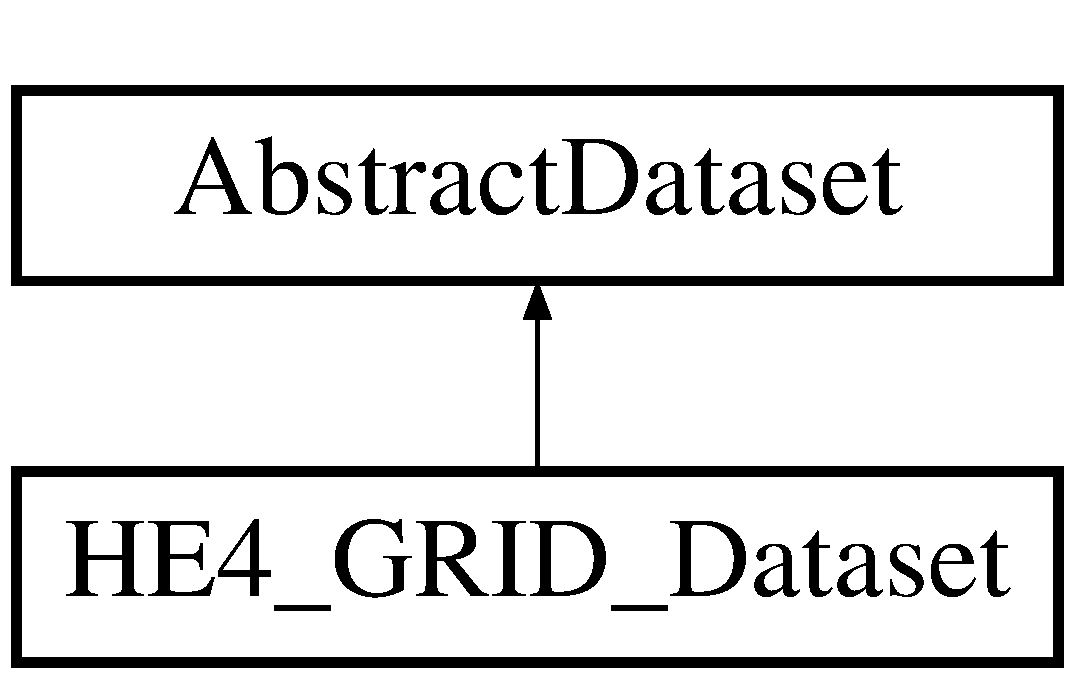
\includegraphics[height=2.000000cm]{classHE4__GRID__Dataset}
\end{center}
\end{figure}
\subsection*{Public Member Functions}
\begin{DoxyCompactItemize}
\item 
virtual CPLErr \hyperlink{classHE4__GRID__Dataset_a553b804b33f2144f131305c3fdea617f}{SetMetaDataList} (GDALDataset $\ast$)
\begin{DoxyCompactList}\small\item\em Set the metadata list for this coverage. \end{DoxyCompactList}\item 
virtual CPLErr \hyperlink{classHE4__GRID__Dataset_a4b37c8d0d47359e11a2dd65fe35f472f}{SetNativeCRS} ()
\begin{DoxyCompactList}\small\item\em Set the Native CRS for a HDF-\/EOS2 Grid dataset. \end{DoxyCompactList}\item 
virtual CPLErr \hyperlink{classHE4__GRID__Dataset_a9afcba857134a8344231286c35a0db51}{SetGeoTransform} ()
\begin{DoxyCompactList}\small\item\em Set the affine GeoTransform matrix for a HDF-\/EOS2 Grid coverage. \end{DoxyCompactList}\item 
virtual CPLErr \hyperlink{classHE4__GRID__Dataset_a140e522053c1010df41e680ee2ded291}{SetGDALDataset} (const int isSimple=0)
\begin{DoxyCompactList}\small\item\em Set the GDALDataset object to HDF-\/EOS2 Grid dataset. \end{DoxyCompactList}\item 
\hyperlink{classHE4__GRID__Dataset_a920e2bb87732d8605f6379d5c7070036}{HE4\_\-GRID\_\-Dataset} (const string \&id, vector$<$ int $>$ \&rBandList)
\begin{DoxyCompactList}\small\item\em Create an HDF-\/EOS2 Grid dataset object. \end{DoxyCompactList}\item 
virtual \hyperlink{classHE4__GRID__Dataset_ae754eaebc441db441e05e0a5e9f9651c}{$\sim$HE4\_\-GRID\_\-Dataset} ()
\begin{DoxyCompactList}\small\item\em Destroy an open \hyperlink{classHE4__GRID__Dataset}{HE4\_\-GRID\_\-Dataset} object. \end{DoxyCompactList}\item 
virtual CPLErr \hyperlink{classHE4__GRID__Dataset_ae45769184c1b4453a81b7809107a6656}{InitialDataset} (const int isSimple=0)
\begin{DoxyCompactList}\small\item\em Initialize the HDF-\/EOS Grid dataset . \end{DoxyCompactList}\end{DoxyCompactItemize}
\subsection*{Static Public Attributes}
\begin{DoxyCompactItemize}
\item 
static string {\bfseries MODIS\_\-Sinusoidal\_\-WKT}
\item 
static string {\bfseries CEA\_\-CRS\_\-WKT}
\end{DoxyCompactItemize}


\subsection{Detailed Description}
\hyperlink{classHE4__GRID__Dataset}{HE4\_\-GRID\_\-Dataset} is a subclass of \hyperlink{classAbstractDataset}{AbstractDataset}, used to process HDF-\/EOS2 Grid coverage. 

To better serve a broader spectrum within the NASA/ECHO with needs for geolocated data, a new format or convention, HDF4-\/EOS was developed. HDF-\/EOS2 supports three geospatial data types: grid, point, and swath.

For grid structures, the HDF-\/EOS library uses the U.S. Geological Survey (USGS) General Cartographic Transformation Package (GCTP) conventions for storing projection information.

\hyperlink{classHE4__GRID__Dataset}{HE4\_\-GRID\_\-Dataset} is a subclass of \hyperlink{classAbstractDataset}{AbstractDataset}, which is used to process MODIS Grid products collection, such as MOD09GQ, MOD13C1 and MOD15A2. 

\subsection{Constructor \& Destructor Documentation}
\hypertarget{classHE4__GRID__Dataset_a920e2bb87732d8605f6379d5c7070036}{
\index{HE4\_\-GRID\_\-Dataset@{HE4\_\-GRID\_\-Dataset}!HE4\_\-GRID\_\-Dataset@{HE4\_\-GRID\_\-Dataset}}
\index{HE4\_\-GRID\_\-Dataset@{HE4\_\-GRID\_\-Dataset}!HE4_GRID_Dataset@{HE4\_\-GRID\_\-Dataset}}
\subsubsection[{HE4\_\-GRID\_\-Dataset}]{\setlength{\rightskip}{0pt plus 5cm}HE4\_\-GRID\_\-Dataset::HE4\_\-GRID\_\-Dataset (
\begin{DoxyParamCaption}
\item[{const string \&}]{id, }
\item[{vector$<$ int $>$ \&}]{rBandList}
\end{DoxyParamCaption}
)}}
\label{classHE4__GRID__Dataset_a920e2bb87732d8605f6379d5c7070036}


Create an HDF-\/EOS2 Grid dataset object. 

This is the accepted method of creating a \hyperlink{classHE4__GRID__Dataset}{HE4\_\-GRID\_\-Dataset} dataset and allocating all resources associated with it.


\begin{DoxyParams}{Parameters}
{\em id} & The coverage identifier.\\
\hline
{\em rBandList} & The field list selected for this coverage. For HDF-\/EOS2 Grid data, only one field in each coverage.\\
\hline
\end{DoxyParams}
\begin{DoxyReturn}{Returns}
A \hyperlink{classHE4__GRID__Dataset}{HE4\_\-GRID\_\-Dataset} object. 
\end{DoxyReturn}
\hypertarget{classHE4__GRID__Dataset_ae754eaebc441db441e05e0a5e9f9651c}{
\index{HE4\_\-GRID\_\-Dataset@{HE4\_\-GRID\_\-Dataset}!$\sim$HE4\_\-GRID\_\-Dataset@{$\sim$HE4\_\-GRID\_\-Dataset}}
\index{$\sim$HE4\_\-GRID\_\-Dataset@{$\sim$HE4\_\-GRID\_\-Dataset}!HE4_GRID_Dataset@{HE4\_\-GRID\_\-Dataset}}
\subsubsection[{$\sim$HE4\_\-GRID\_\-Dataset}]{\setlength{\rightskip}{0pt plus 5cm}HE4\_\-GRID\_\-Dataset::$\sim$HE4\_\-GRID\_\-Dataset (
\begin{DoxyParamCaption}
{}
\end{DoxyParamCaption}
)\hspace{0.3cm}{\ttfamily  \mbox{[}virtual\mbox{]}}}}
\label{classHE4__GRID__Dataset_ae754eaebc441db441e05e0a5e9f9651c}


Destroy an open \hyperlink{classHE4__GRID__Dataset}{HE4\_\-GRID\_\-Dataset} object. 

This is the accepted method of closing a \hyperlink{classHE4__GRID__Dataset}{HE4\_\-GRID\_\-Dataset} dataset and deallocating all resources associated with it. 

\subsection{Member Function Documentation}
\hypertarget{classHE4__GRID__Dataset_ae45769184c1b4453a81b7809107a6656}{
\index{HE4\_\-GRID\_\-Dataset@{HE4\_\-GRID\_\-Dataset}!InitialDataset@{InitialDataset}}
\index{InitialDataset@{InitialDataset}!HE4_GRID_Dataset@{HE4\_\-GRID\_\-Dataset}}
\subsubsection[{InitialDataset}]{\setlength{\rightskip}{0pt plus 5cm}CPLErr HE4\_\-GRID\_\-Dataset::InitialDataset (
\begin{DoxyParamCaption}
\item[{const int}]{isSimple = {\ttfamily 0}}
\end{DoxyParamCaption}
)\hspace{0.3cm}{\ttfamily  \mbox{[}virtual\mbox{]}}}}
\label{classHE4__GRID__Dataset_ae45769184c1b4453a81b7809107a6656}


Initialize the HDF-\/EOS Grid dataset . 

This method is the implementation for initializing a HDF-\/EOS2 Grid dataset. Within this method, \hyperlink{classHE4__GRID__Dataset_a4b37c8d0d47359e11a2dd65fe35f472f}{SetNativeCRS()}, \hyperlink{classHE4__GRID__Dataset_a9afcba857134a8344231286c35a0db51}{SetGeoTransform()} and \hyperlink{classHE4__GRID__Dataset_a140e522053c1010df41e680ee2ded291}{SetGDALDataset()} will be called to initialize an HDF-\/EOS2 Grid dataset. $\ast$ The coverage type of HDF-\/EOS Swath data is set to \char`\"{}RectifiedDataset\char`\"{}.


\begin{DoxyParams}{Parameters}
{\em isSimple} & The WCS request type. When user executing a DescribeCoverage request, isSimple is set to 1, and for GetCoverage, is set to 0.\\
\hline
\end{DoxyParams}
\begin{DoxyReturn}{Returns}
CE\_\-None on success or CE\_\-Failure on failure. 
\end{DoxyReturn}


Reimplemented from \hyperlink{classAbstractDataset_a45924895c6bf26c7f75d503b8f6e388a}{AbstractDataset}.

\hypertarget{classHE4__GRID__Dataset_a140e522053c1010df41e680ee2ded291}{
\index{HE4\_\-GRID\_\-Dataset@{HE4\_\-GRID\_\-Dataset}!SetGDALDataset@{SetGDALDataset}}
\index{SetGDALDataset@{SetGDALDataset}!HE4_GRID_Dataset@{HE4\_\-GRID\_\-Dataset}}
\subsubsection[{SetGDALDataset}]{\setlength{\rightskip}{0pt plus 5cm}CPLErr HE4\_\-GRID\_\-Dataset::SetGDALDataset (
\begin{DoxyParamCaption}
\item[{const int}]{isSimple = {\ttfamily 0}}
\end{DoxyParamCaption}
)\hspace{0.3cm}{\ttfamily  \mbox{[}virtual\mbox{]}}}}
\label{classHE4__GRID__Dataset_a140e522053c1010df41e680ee2ded291}


Set the GDALDataset object to HDF-\/EOS2 Grid dataset. 

This method is used to set the HDF-\/EOS2 Grid dataset based on GDAL class VRTDataset.


\begin{DoxyParams}{Parameters}
{\em isSimple} & the WCS request type. When user executing a DescribeCoverage request, isSimple is set to 1, and for GetCoverage, is set to 0.\\
\hline
\end{DoxyParams}
\begin{DoxyReturn}{Returns}
CE\_\-None on success or CE\_\-Failure on failure. 
\end{DoxyReturn}


Reimplemented from \hyperlink{classAbstractDataset_a93bd80bfa48ad45ea53599f289406287}{AbstractDataset}.

\hypertarget{classHE4__GRID__Dataset_a9afcba857134a8344231286c35a0db51}{
\index{HE4\_\-GRID\_\-Dataset@{HE4\_\-GRID\_\-Dataset}!SetGeoTransform@{SetGeoTransform}}
\index{SetGeoTransform@{SetGeoTransform}!HE4_GRID_Dataset@{HE4\_\-GRID\_\-Dataset}}
\subsubsection[{SetGeoTransform}]{\setlength{\rightskip}{0pt plus 5cm}CPLErr HE4\_\-GRID\_\-Dataset::SetGeoTransform (
\begin{DoxyParamCaption}
{}
\end{DoxyParamCaption}
)\hspace{0.3cm}{\ttfamily  \mbox{[}virtual\mbox{]}}}}
\label{classHE4__GRID__Dataset_a9afcba857134a8344231286c35a0db51}


Set the affine GeoTransform matrix for a HDF-\/EOS2 Grid coverage. 

The method will set a GeoTransform matrix for a HDF-\/EOS2 Grid coverage by parsing and analyzing the metadata of HDF-\/EOS2 Grid data granule.

The CRS for the bounding box is EPSG:4326.

\begin{DoxyReturn}{Returns}
CE\_\-None on success or CE\_\-Failure on failure. 
\end{DoxyReturn}


Reimplemented from \hyperlink{classAbstractDataset_a1d79fc347de75acd57b18c80b9614369}{AbstractDataset}.

\hypertarget{classHE4__GRID__Dataset_a553b804b33f2144f131305c3fdea617f}{
\index{HE4\_\-GRID\_\-Dataset@{HE4\_\-GRID\_\-Dataset}!SetMetaDataList@{SetMetaDataList}}
\index{SetMetaDataList@{SetMetaDataList}!HE4_GRID_Dataset@{HE4\_\-GRID\_\-Dataset}}
\subsubsection[{SetMetaDataList}]{\setlength{\rightskip}{0pt plus 5cm}CPLErr HE4\_\-GRID\_\-Dataset::SetMetaDataList (
\begin{DoxyParamCaption}
\item[{GDALDataset $\ast$}]{hSrcDS}
\end{DoxyParamCaption}
)\hspace{0.3cm}{\ttfamily  \mbox{[}virtual\mbox{]}}}}
\label{classHE4__GRID__Dataset_a553b804b33f2144f131305c3fdea617f}


Set the metadata list for this coverage. 

The method will set the metadata list for the coverage based on its corresponding GDALDataset object.


\begin{DoxyParams}{Parameters}
{\em hSrc} & the GDALDataset object corresponding to coverage.\\
\hline
\end{DoxyParams}
\begin{DoxyReturn}{Returns}
CE\_\-None on success or CE\_\-Failure on failure. 
\end{DoxyReturn}


Reimplemented from \hyperlink{classAbstractDataset_af3f0b55b14f660b79751bf88489a2c10}{AbstractDataset}.

\hypertarget{classHE4__GRID__Dataset_a4b37c8d0d47359e11a2dd65fe35f472f}{
\index{HE4\_\-GRID\_\-Dataset@{HE4\_\-GRID\_\-Dataset}!SetNativeCRS@{SetNativeCRS}}
\index{SetNativeCRS@{SetNativeCRS}!HE4_GRID_Dataset@{HE4\_\-GRID\_\-Dataset}}
\subsubsection[{SetNativeCRS}]{\setlength{\rightskip}{0pt plus 5cm}CPLErr HE4\_\-GRID\_\-Dataset::SetNativeCRS (
\begin{DoxyParamCaption}
{}
\end{DoxyParamCaption}
)\hspace{0.3cm}{\ttfamily  \mbox{[}virtual\mbox{]}}}}
\label{classHE4__GRID__Dataset_a4b37c8d0d47359e11a2dd65fe35f472f}


Set the Native CRS for a HDF-\/EOS2 Grid dataset. 

The method will set the CRS for a HDF-\/EOS2 Grid dataset as an native CRS.

\begin{DoxyReturn}{Returns}
CE\_\-None on success or CE\_\-Failure on failure. 
\end{DoxyReturn}


Reimplemented from \hyperlink{classAbstractDataset_acfac922d16e5edf51066169bd6ff28ec}{AbstractDataset}.



\subsection{Member Data Documentation}
\hypertarget{classHE4__GRID__Dataset_a6e87bb6abdb928a2af04232bef254667}{
\index{HE4\_\-GRID\_\-Dataset@{HE4\_\-GRID\_\-Dataset}!CEA\_\-CRS\_\-WKT@{CEA\_\-CRS\_\-WKT}}
\index{CEA\_\-CRS\_\-WKT@{CEA\_\-CRS\_\-WKT}!HE4_GRID_Dataset@{HE4\_\-GRID\_\-Dataset}}
\subsubsection[{CEA\_\-CRS\_\-WKT}]{\setlength{\rightskip}{0pt plus 5cm}string HE4\_\-GRID\_\-Dataset::CEA\_\-CRS\_\-WKT\hspace{0.3cm}{\ttfamily  \mbox{[}static\mbox{]}}}}
\label{classHE4__GRID__Dataset_a6e87bb6abdb928a2af04232bef254667}
{\bfseries Initial value:}
\begin{DoxyCode}
"PROJCS[\"NSIDC EASE-Grid Global\", \
                GEOGCS[\"Unspecified datum based upon the International 1924 Auth
      alic Sphere\", \
                        DATUM[\"Not_specified_based_on_International_1924_Authali
      c_Sphere\", \
                                SPHEROID[\"International 1924 Authalic Sphere\",6
      371228,0, \
                                        AUTHORITY[\"EPSG\",\"7057\"]], \
                                AUTHORITY[\"EPSG\",\"6053\"]], \
                        PRIMEM[\"Greenwich\",0, \
                                AUTHORITY[\"EPSG\",\"8901\"]], \
                        UNIT[\"degree\",0.01745329251994328, \
                                AUTHORITY[\"EPSG\",\"9122\"]], \
                        AUTHORITY[\"EPSG\",\"4053\"]], \
                UNIT[\"metre\",1, \
                        AUTHORITY[\"EPSG\",\"9001\"]], \
                PROJECTION[\"Cylindrical_Equal_Area\"], \
                PARAMETER[\"standard_parallel_1\",30], \
                PARAMETER[\"central_meridian\",0], \
                PARAMETER[\"false_easting\",0], \
                PARAMETER[\"false_northing\",0], \
                AUTHORITY[\"EPSG\",\"3410\"], \
                AXIS[\"X\",EAST], \
                AXIS[\"Y\",NORTH]]"
\end{DoxyCode}
\hypertarget{classHE4__GRID__Dataset_ab96a75584a7775cc29c52b3004a31d3e}{
\index{HE4\_\-GRID\_\-Dataset@{HE4\_\-GRID\_\-Dataset}!MODIS\_\-Sinusoidal\_\-WKT@{MODIS\_\-Sinusoidal\_\-WKT}}
\index{MODIS\_\-Sinusoidal\_\-WKT@{MODIS\_\-Sinusoidal\_\-WKT}!HE4_GRID_Dataset@{HE4\_\-GRID\_\-Dataset}}
\subsubsection[{MODIS\_\-Sinusoidal\_\-WKT}]{\setlength{\rightskip}{0pt plus 5cm}string HE4\_\-GRID\_\-Dataset::MODIS\_\-Sinusoidal\_\-WKT\hspace{0.3cm}{\ttfamily  \mbox{[}static\mbox{]}}}}
\label{classHE4__GRID__Dataset_ab96a75584a7775cc29c52b3004a31d3e}
{\bfseries Initial value:}
\begin{DoxyCode}
"PROJCS[\"MODIS Sinusoidal\", \
    GEOGCS[\"WGS 84\", \
        DATUM[\"WGS_1984\", \
            SPHEROID[\"WGS 84\",6378137,298.257223563, \
                AUTHORITY[\"EPSG\",\"7030\"]], \
            AUTHORITY[\"EPSG\",\"6326\"]], \
        PRIMEM[\"Greenwich\",0, \
            AUTHORITY[\"EPSG\",\"8901\"]], \
        UNIT[\"degree\",0.01745329251994328, \
            AUTHORITY[\"EPSG\",\"9122\"]], \
        AUTHORITY[\"EPSG\",\"4326\"]], \
    PROJECTION[\"Sinusoidal\"], \
    PARAMETER[\"false_easting\",0.0], \
    PARAMETER[\"false_northing\",0.0], \
    PARAMETER[\"central_meridian\",0.0], \
    PARAMETER[\"semi_major\",6371007.181], \
    PARAMETER[\"semi_minor\",6371007.181], \
    UNIT[\"m\",1.0], \
    AUTHORITY[\"SR-ORG\",\"6974\"]]"
\end{DoxyCode}


The documentation for this class was generated from the following files:\begin{DoxyCompactItemize}
\item 
HE4\_\-GRID\_\-Dataset.h\item 
HE4\_\-GRID\_\-Dataset.cpp\end{DoxyCompactItemize}

\hypertarget{classHE4__SWATH__Dataset}{
\section{HE4\_\-SWATH\_\-Dataset Class Reference}
\label{classHE4__SWATH__Dataset}\index{HE4\_\-SWATH\_\-Dataset@{HE4\_\-SWATH\_\-Dataset}}
}


\hyperlink{classHE4__SWATH__Dataset}{HE4\_\-SWATH\_\-Dataset} is a subclass of \hyperlink{classAbstractDataset}{AbstractDataset}, used to process HDF-\/EOS2 Swath coverage.  




{\ttfamily \#include \char`\"{}HE4\_\-SWATH\_\-Dataset.h\char`\"{}}

Inheritance diagram for HE4\_\-SWATH\_\-Dataset:\begin{figure}[H]
\begin{center}
\leavevmode
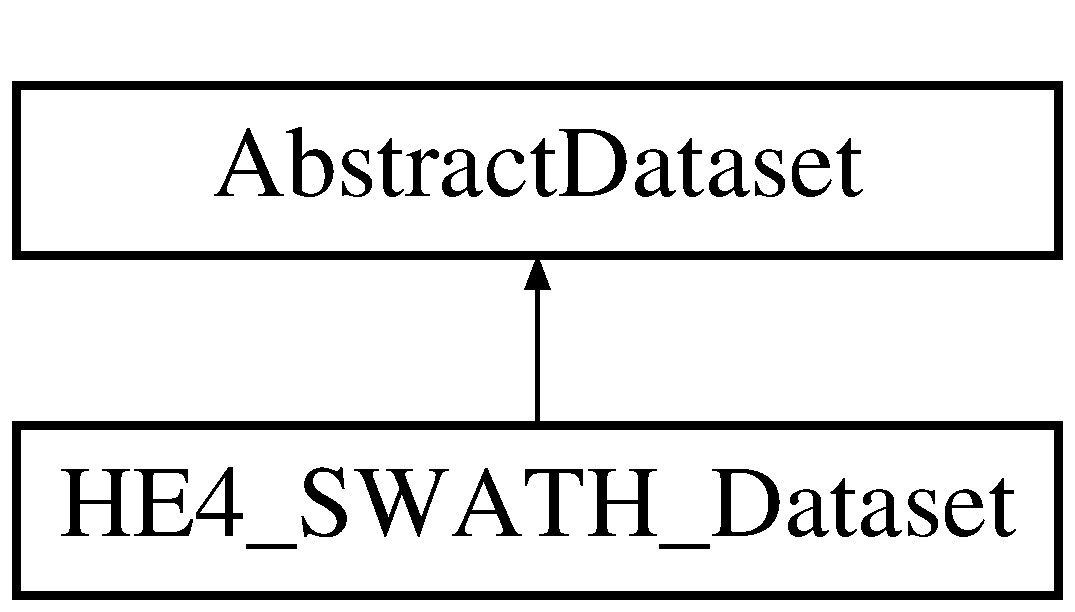
\includegraphics[height=2.000000cm]{classHE4__SWATH__Dataset}
\end{center}
\end{figure}
\subsection*{Public Member Functions}
\begin{DoxyCompactItemize}
\item 
virtual CPLErr \hyperlink{classHE4__SWATH__Dataset_a898be04259ed34592cbff87b2dd2680c}{SetGeoTransform} ()
\begin{DoxyCompactList}\small\item\em Set the affine GeoTransform matrix for a HDF-\/EOS2 Swath coverage. \end{DoxyCompactList}\item 
virtual CPLErr \hyperlink{classHE4__SWATH__Dataset_a71289ad4d22695120264b190e9170eb1}{SetMetaDataList} (GDALDataset $\ast$)
\begin{DoxyCompactList}\small\item\em Set the metadata list for this coverage. \end{DoxyCompactList}\item 
virtual CPLErr \hyperlink{classHE4__SWATH__Dataset_abc9a1e86eba1e386e38e3771e4102df4}{SetNativeCRS} ()
\begin{DoxyCompactList}\small\item\em Set the Native CRS for a HDF-\/EOS2 Swath dataset. \end{DoxyCompactList}\item 
virtual CPLErr \hyperlink{classHE4__SWATH__Dataset_aba0769c876c341494ba043f5cbcdef9a}{SetGDALDataset} (const int isSimple=0)
\begin{DoxyCompactList}\small\item\em Set the GDALDataset object to HDF-\/EOS2 Swath dataset. \end{DoxyCompactList}\item 
virtual CPLErr \hyperlink{classHE4__SWATH__Dataset_ac65fb00ef5ac627fb996e46442c07444}{InitialDataset} (const int isSimple=0)
\begin{DoxyCompactList}\small\item\em Initialize the HDF-\/EOS Swath dataset . \end{DoxyCompactList}\item 
\hyperlink{classHE4__SWATH__Dataset_a354e9e0923628cbfa6f7e6864afeba36}{HE4\_\-SWATH\_\-Dataset} (const string \&id, vector$<$ int $>$ \&rBandList)
\begin{DoxyCompactList}\small\item\em Create an HDF-\/EOS Swath dataset object. \end{DoxyCompactList}\item 
virtual \hyperlink{classHE4__SWATH__Dataset_a084f204e8cd2c7401b84bbd6aa98fd94}{$\sim$HE4\_\-SWATH\_\-Dataset} ()
\begin{DoxyCompactList}\small\item\em Destroy an open \hyperlink{classHE4__SWATH__Dataset}{HE4\_\-SWATH\_\-Dataset} object. \end{DoxyCompactList}\item 
virtual int \hyperlink{classHE4__SWATH__Dataset_acbe2ea029124c791fc8fe2b9e68a8bf8}{GetImageXSize} ()
\begin{DoxyCompactList}\small\item\em Fetch coverage width in pixels. \end{DoxyCompactList}\item 
virtual int \hyperlink{classHE4__SWATH__Dataset_ab8450ad5ae44927bb8aef7dba5bc1af8}{GetImageYSize} ()
\begin{DoxyCompactList}\small\item\em Fetch coverage height in pixels. \end{DoxyCompactList}\end{DoxyCompactItemize}
\subsection*{Protected Attributes}
\begin{DoxyCompactItemize}
\item 
\hypertarget{classHE4__SWATH__Dataset_ae158131d053ed98cc48f8d8be3fe5481}{
int {\bfseries mi\_\-RectifiedImageXSize}}
\label{classHE4__SWATH__Dataset_ae158131d053ed98cc48f8d8be3fe5481}

\item 
\hypertarget{classHE4__SWATH__Dataset_a234f2289c231f9c4bb2fa181ab28220c}{
int {\bfseries mi\_\-RectifiedImageYSize}}
\label{classHE4__SWATH__Dataset_a234f2289c231f9c4bb2fa181ab28220c}

\end{DoxyCompactItemize}


\subsection{Detailed Description}
\hyperlink{classHE4__SWATH__Dataset}{HE4\_\-SWATH\_\-Dataset} is a subclass of \hyperlink{classAbstractDataset}{AbstractDataset}, used to process HDF-\/EOS2 Swath coverage. 

The Swath concept for HDF-\/EOS is based on a typical satellite swath, where an instrument takes a series of scans perpendicular to the ground track of the satellite as it moves along that ground track.

The HDF-\/EOS2 data view of a swath is one where the data is ordered by time or a time-\/like variable (e.g., scan line counter). The data stored for every time entry can consist of time, geolocation (latitude, longitude), scalar values, 1D arrays of values (scan lines or profiles), or 2D arrays of values (multiple channel scan lines).

\hyperlink{classHE4__SWATH__Dataset}{HE4\_\-SWATH\_\-Dataset} is a subclass of \hyperlink{classAbstractDataset}{AbstractDataset}, which is used to process MODIS Swath products collection, such as MOD021KM, MYD02HKM and MOD02QKM. 

\subsection{Constructor \& Destructor Documentation}
\hypertarget{classHE4__SWATH__Dataset_a354e9e0923628cbfa6f7e6864afeba36}{
\index{HE4\_\-SWATH\_\-Dataset@{HE4\_\-SWATH\_\-Dataset}!HE4\_\-SWATH\_\-Dataset@{HE4\_\-SWATH\_\-Dataset}}
\index{HE4\_\-SWATH\_\-Dataset@{HE4\_\-SWATH\_\-Dataset}!HE4_SWATH_Dataset@{HE4\_\-SWATH\_\-Dataset}}
\subsubsection[{HE4\_\-SWATH\_\-Dataset}]{\setlength{\rightskip}{0pt plus 5cm}HE4\_\-SWATH\_\-Dataset::HE4\_\-SWATH\_\-Dataset (
\begin{DoxyParamCaption}
\item[{const string \&}]{id, }
\item[{vector$<$ int $>$ \&}]{rBandList}
\end{DoxyParamCaption}
)}}
\label{classHE4__SWATH__Dataset_a354e9e0923628cbfa6f7e6864afeba36}


Create an HDF-\/EOS Swath dataset object. 

This is the accepted method of creating a \hyperlink{classHE4__SWATH__Dataset}{HE4\_\-SWATH\_\-Dataset} dataset and allocating all resources associated with it.


\begin{DoxyParams}{Parameters}
{\em id} & The coverage identifier.\\
\hline
{\em rBandList} & The field list selected for this coverage. For HDF-\/EOS Swath data, the user may choose multiple range and execute range subset operation.\\
\hline
\end{DoxyParams}
\begin{DoxyReturn}{Returns}
A \hyperlink{classHE4__SWATH__Dataset}{HE4\_\-SWATH\_\-Dataset} object. 
\end{DoxyReturn}
\hypertarget{classHE4__SWATH__Dataset_a084f204e8cd2c7401b84bbd6aa98fd94}{
\index{HE4\_\-SWATH\_\-Dataset@{HE4\_\-SWATH\_\-Dataset}!$\sim$HE4\_\-SWATH\_\-Dataset@{$\sim$HE4\_\-SWATH\_\-Dataset}}
\index{$\sim$HE4\_\-SWATH\_\-Dataset@{$\sim$HE4\_\-SWATH\_\-Dataset}!HE4_SWATH_Dataset@{HE4\_\-SWATH\_\-Dataset}}
\subsubsection[{$\sim$HE4\_\-SWATH\_\-Dataset}]{\setlength{\rightskip}{0pt plus 5cm}HE4\_\-SWATH\_\-Dataset::$\sim$HE4\_\-SWATH\_\-Dataset (
\begin{DoxyParamCaption}
{}
\end{DoxyParamCaption}
)\hspace{0.3cm}{\ttfamily  \mbox{[}virtual\mbox{]}}}}
\label{classHE4__SWATH__Dataset_a084f204e8cd2c7401b84bbd6aa98fd94}


Destroy an open \hyperlink{classHE4__SWATH__Dataset}{HE4\_\-SWATH\_\-Dataset} object. 

This is the accepted method of closing a \hyperlink{classHE4__SWATH__Dataset}{HE4\_\-SWATH\_\-Dataset} dataset and deallocating all resources associated with it. 

\subsection{Member Function Documentation}
\hypertarget{classHE4__SWATH__Dataset_acbe2ea029124c791fc8fe2b9e68a8bf8}{
\index{HE4\_\-SWATH\_\-Dataset@{HE4\_\-SWATH\_\-Dataset}!GetImageXSize@{GetImageXSize}}
\index{GetImageXSize@{GetImageXSize}!HE4_SWATH_Dataset@{HE4\_\-SWATH\_\-Dataset}}
\subsubsection[{GetImageXSize}]{\setlength{\rightskip}{0pt plus 5cm}virtual int HE4\_\-SWATH\_\-Dataset::GetImageXSize (
\begin{DoxyParamCaption}
{}
\end{DoxyParamCaption}
)\hspace{0.3cm}{\ttfamily  \mbox{[}inline, virtual\mbox{]}}}}
\label{classHE4__SWATH__Dataset_acbe2ea029124c791fc8fe2b9e68a8bf8}


Fetch coverage width in pixels. 

The method will return the width of coverage in pixels. GDAL API GetRasterXSize() will be called to generate the width value.

\begin{DoxyReturn}{Returns}
the width in pixels of raster bands in this coverage. 
\end{DoxyReturn}


Reimplemented from \hyperlink{classAbstractDataset_a950e120c5a1e9fa06ee5b02ed4fc6c42}{AbstractDataset}.

\hypertarget{classHE4__SWATH__Dataset_ab8450ad5ae44927bb8aef7dba5bc1af8}{
\index{HE4\_\-SWATH\_\-Dataset@{HE4\_\-SWATH\_\-Dataset}!GetImageYSize@{GetImageYSize}}
\index{GetImageYSize@{GetImageYSize}!HE4_SWATH_Dataset@{HE4\_\-SWATH\_\-Dataset}}
\subsubsection[{GetImageYSize}]{\setlength{\rightskip}{0pt plus 5cm}virtual int HE4\_\-SWATH\_\-Dataset::GetImageYSize (
\begin{DoxyParamCaption}
{}
\end{DoxyParamCaption}
)\hspace{0.3cm}{\ttfamily  \mbox{[}inline, virtual\mbox{]}}}}
\label{classHE4__SWATH__Dataset_ab8450ad5ae44927bb8aef7dba5bc1af8}


Fetch coverage height in pixels. 

The method will return the height of coverage in pixels. GDAL API GetRasterYSize() will be called to generate the height value.

\begin{DoxyReturn}{Returns}
the height in pixels of raster bands in this coverage. 
\end{DoxyReturn}


Reimplemented from \hyperlink{classAbstractDataset_a4f7ceb09ad968d28a5282c7652fb6975}{AbstractDataset}.

\hypertarget{classHE4__SWATH__Dataset_ac65fb00ef5ac627fb996e46442c07444}{
\index{HE4\_\-SWATH\_\-Dataset@{HE4\_\-SWATH\_\-Dataset}!InitialDataset@{InitialDataset}}
\index{InitialDataset@{InitialDataset}!HE4_SWATH_Dataset@{HE4\_\-SWATH\_\-Dataset}}
\subsubsection[{InitialDataset}]{\setlength{\rightskip}{0pt plus 5cm}CPLErr HE4\_\-SWATH\_\-Dataset::InitialDataset (
\begin{DoxyParamCaption}
\item[{const int}]{isSimple = {\ttfamily 0}}
\end{DoxyParamCaption}
)\hspace{0.3cm}{\ttfamily  \mbox{[}virtual\mbox{]}}}}
\label{classHE4__SWATH__Dataset_ac65fb00ef5ac627fb996e46442c07444}


Initialize the HDF-\/EOS Swath dataset . 

This method is the implementation for initializing a HDF-\/EOS Swath dataset. Within this method, \hyperlink{classHE4__SWATH__Dataset_abc9a1e86eba1e386e38e3771e4102df4}{SetNativeCRS()}, \hyperlink{classHE4__SWATH__Dataset_a898be04259ed34592cbff87b2dd2680c}{SetGeoTransform()} and \hyperlink{classHE4__SWATH__Dataset_aba0769c876c341494ba043f5cbcdef9a}{SetGDALDataset()} will be called to initialize an HDF-\/EOS Swath dataset. The coverage type of HDF-\/EOS Swath data is set to \char`\"{}ReferenceableDataset\char`\"{}.


\begin{DoxyParams}{Parameters}
{\em isSimple} & the WCS request type. When user executing a DescribeCoverage request, isSimple is set to 1, and for GetCoverage, is set to 0.\\
\hline
\end{DoxyParams}
\begin{DoxyReturn}{Returns}
CE\_\-None on success or CE\_\-Failure on failure. 
\end{DoxyReturn}


Reimplemented from \hyperlink{classAbstractDataset_a45924895c6bf26c7f75d503b8f6e388a}{AbstractDataset}.

\hypertarget{classHE4__SWATH__Dataset_aba0769c876c341494ba043f5cbcdef9a}{
\index{HE4\_\-SWATH\_\-Dataset@{HE4\_\-SWATH\_\-Dataset}!SetGDALDataset@{SetGDALDataset}}
\index{SetGDALDataset@{SetGDALDataset}!HE4_SWATH_Dataset@{HE4\_\-SWATH\_\-Dataset}}
\subsubsection[{SetGDALDataset}]{\setlength{\rightskip}{0pt plus 5cm}CPLErr HE4\_\-SWATH\_\-Dataset::SetGDALDataset (
\begin{DoxyParamCaption}
\item[{const int}]{isSimple = {\ttfamily 0}}
\end{DoxyParamCaption}
)\hspace{0.3cm}{\ttfamily  \mbox{[}virtual\mbox{]}}}}
\label{classHE4__SWATH__Dataset_aba0769c876c341494ba043f5cbcdef9a}


Set the GDALDataset object to HDF-\/EOS2 Swath dataset. 

This method is used to set the HDF-\/EOS2 Swath dataset based on GDAL class VRTDataset.


\begin{DoxyParams}{Parameters}
{\em isSimple} & the WCS request type. When user executing a DescribeCoverage request, isSimple is set to 1, and for GetCoverage, is set to 0.\\
\hline
\end{DoxyParams}
\begin{DoxyReturn}{Returns}
CE\_\-None on success or CE\_\-Failure on failure. 
\end{DoxyReturn}


Reimplemented from \hyperlink{classAbstractDataset_a93bd80bfa48ad45ea53599f289406287}{AbstractDataset}.

\hypertarget{classHE4__SWATH__Dataset_a898be04259ed34592cbff87b2dd2680c}{
\index{HE4\_\-SWATH\_\-Dataset@{HE4\_\-SWATH\_\-Dataset}!SetGeoTransform@{SetGeoTransform}}
\index{SetGeoTransform@{SetGeoTransform}!HE4_SWATH_Dataset@{HE4\_\-SWATH\_\-Dataset}}
\subsubsection[{SetGeoTransform}]{\setlength{\rightskip}{0pt plus 5cm}CPLErr HE4\_\-SWATH\_\-Dataset::SetGeoTransform (
\begin{DoxyParamCaption}
{}
\end{DoxyParamCaption}
)\hspace{0.3cm}{\ttfamily  \mbox{[}virtual\mbox{]}}}}
\label{classHE4__SWATH__Dataset_a898be04259ed34592cbff87b2dd2680c}


Set the affine GeoTransform matrix for a HDF-\/EOS2 Swath coverage. 

The method will set a GeoTransform matrix for a HDF-\/EOS2 Grid coverage by parsing and analyzing the metadata of HDF-\/EOS2 Grid data granule. If granule metadata do not include bounding box extent, GDAL\_\-GCP will be used to deduce the bounding box and set the GeoTransform accordingly.

\begin{DoxyReturn}{Returns}
CE\_\-None on success or CE\_\-Failure on failure. 
\end{DoxyReturn}


Reimplemented from \hyperlink{classAbstractDataset_a1d79fc347de75acd57b18c80b9614369}{AbstractDataset}.

\hypertarget{classHE4__SWATH__Dataset_a71289ad4d22695120264b190e9170eb1}{
\index{HE4\_\-SWATH\_\-Dataset@{HE4\_\-SWATH\_\-Dataset}!SetMetaDataList@{SetMetaDataList}}
\index{SetMetaDataList@{SetMetaDataList}!HE4_SWATH_Dataset@{HE4\_\-SWATH\_\-Dataset}}
\subsubsection[{SetMetaDataList}]{\setlength{\rightskip}{0pt plus 5cm}CPLErr HE4\_\-SWATH\_\-Dataset::SetMetaDataList (
\begin{DoxyParamCaption}
\item[{GDALDataset $\ast$}]{hSrcDS}
\end{DoxyParamCaption}
)\hspace{0.3cm}{\ttfamily  \mbox{[}virtual\mbox{]}}}}
\label{classHE4__SWATH__Dataset_a71289ad4d22695120264b190e9170eb1}


Set the metadata list for this coverage. 

The method will set the metadata list for the coverage based on its corresponding GDALDataset object.


\begin{DoxyParams}{Parameters}
{\em hSrc} & the GDALDataset object corresponding to coverage.\\
\hline
\end{DoxyParams}
\begin{DoxyReturn}{Returns}
CE\_\-None on success or CE\_\-Failure on failure. 
\end{DoxyReturn}


Reimplemented from \hyperlink{classAbstractDataset_af3f0b55b14f660b79751bf88489a2c10}{AbstractDataset}.

\hypertarget{classHE4__SWATH__Dataset_abc9a1e86eba1e386e38e3771e4102df4}{
\index{HE4\_\-SWATH\_\-Dataset@{HE4\_\-SWATH\_\-Dataset}!SetNativeCRS@{SetNativeCRS}}
\index{SetNativeCRS@{SetNativeCRS}!HE4_SWATH_Dataset@{HE4\_\-SWATH\_\-Dataset}}
\subsubsection[{SetNativeCRS}]{\setlength{\rightskip}{0pt plus 5cm}CPLErr HE4\_\-SWATH\_\-Dataset::SetNativeCRS (
\begin{DoxyParamCaption}
{}
\end{DoxyParamCaption}
)\hspace{0.3cm}{\ttfamily  \mbox{[}virtual\mbox{]}}}}
\label{classHE4__SWATH__Dataset_abc9a1e86eba1e386e38e3771e4102df4}


Set the Native CRS for a HDF-\/EOS2 Swath dataset. 

The method will set the CRS for a HDF-\/EOS2 Grid dataset as an native CRS. Since the coordinates recorded in HDF-\/EOS2 Swath granule belong to geographic CRS, EPSG:4326 CRS are assigned to HDF-\/EOS2 Swath dataset.

\begin{DoxyReturn}{Returns}
CE\_\-None on success or CE\_\-Failure on failure. 
\end{DoxyReturn}


Reimplemented from \hyperlink{classAbstractDataset_acfac922d16e5edf51066169bd6ff28ec}{AbstractDataset}.



The documentation for this class was generated from the following files:\begin{DoxyCompactItemize}
\item 
HE4\_\-SWATH\_\-Dataset.h\item 
HE4\_\-SWATH\_\-Dataset.cpp\end{DoxyCompactItemize}

\hypertarget{classHE5__GRID__Dataset}{
\section{HE5\_\-GRID\_\-Dataset Class Reference}
\label{classHE5__GRID__Dataset}\index{HE5\_\-GRID\_\-Dataset@{HE5\_\-GRID\_\-Dataset}}
}


\hyperlink{classHE5__GRID__Dataset}{HE5\_\-GRID\_\-Dataset} is a subclass of \hyperlink{classAbstractDataset}{AbstractDataset}, used to process HDF-\/EOS5 Grid coverage.  




{\ttfamily \#include \char`\"{}HE5\_\-GRID\_\-Dataset.h\char`\"{}}

Inheritance diagram for HE5\_\-GRID\_\-Dataset:\begin{figure}[H]
\begin{center}
\leavevmode
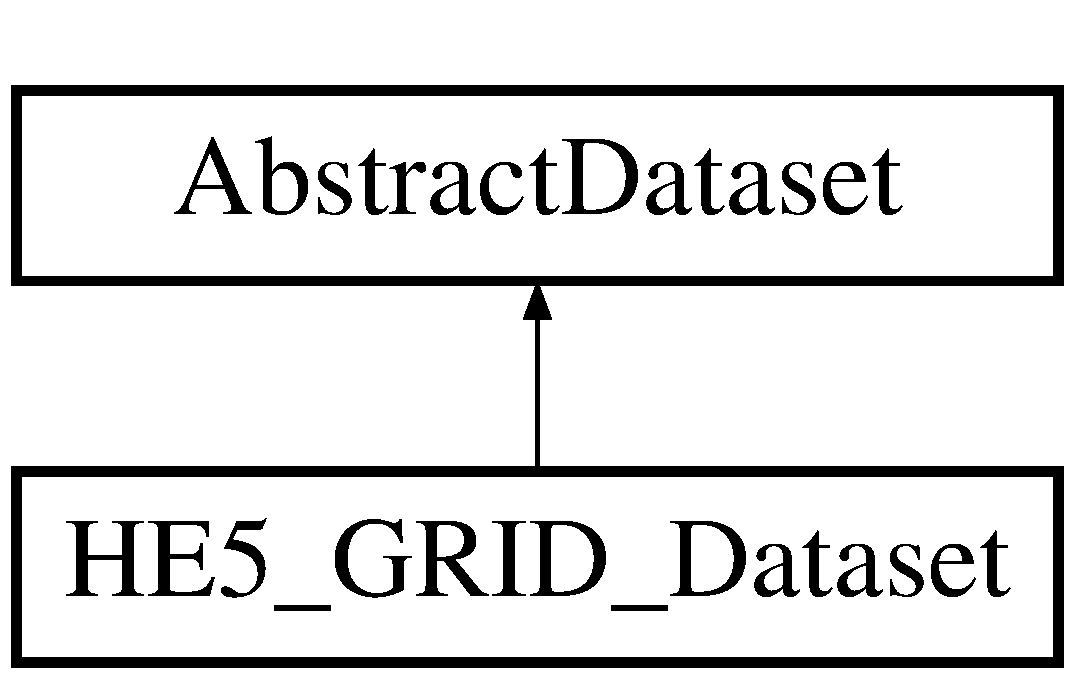
\includegraphics[height=2.000000cm]{classHE5__GRID__Dataset}
\end{center}
\end{figure}
\subsection*{Public Member Functions}
\begin{DoxyCompactItemize}
\item 
\hyperlink{classHE5__GRID__Dataset_ac0112c68e36c333ecd5674ed09949eee}{HE5\_\-GRID\_\-Dataset} (const string \&id, vector$<$ int $>$ \&rBandList)
\begin{DoxyCompactList}\small\item\em Create an HDF-\/EOS5 Grid dataset object. \end{DoxyCompactList}\item 
virtual \hyperlink{classHE5__GRID__Dataset_a53a2be006884df9ba95a58d9db1aa0fc}{$\sim$HE5\_\-GRID\_\-Dataset} ()
\begin{DoxyCompactList}\small\item\em Destroy an open \hyperlink{classHE5__GRID__Dataset}{HE5\_\-GRID\_\-Dataset} object. \end{DoxyCompactList}\item 
virtual CPLErr \hyperlink{classHE5__GRID__Dataset_aab2d7ffe28f4b1fda41f5ec10a33e8a3}{SetMetaDataList} (GDALDataset $\ast$)
\begin{DoxyCompactList}\small\item\em Set the metadata list for this coverage. \end{DoxyCompactList}\item 
virtual CPLErr \hyperlink{classHE5__GRID__Dataset_a2bdcf5b88ef679f6fcfd7cd909e56bb7}{SetNativeCRS} ()
\begin{DoxyCompactList}\small\item\em Set the Native CRS for a HDF-\/EOS5 Grid dataset. \end{DoxyCompactList}\item 
virtual CPLErr \hyperlink{classHE5__GRID__Dataset_ab20ae6fe7456bb91c0cd8b4fdb6db1f1}{SetGeoTransform} ()
\begin{DoxyCompactList}\small\item\em Set the affine GeoTransform matrix for a HDF-\/EOS5 Grid coverage. \end{DoxyCompactList}\item 
virtual CPLErr \hyperlink{classHE5__GRID__Dataset_afc38747b72c0862de45f897867903e57}{SetGDALDataset} (const int isSimple=0)
\begin{DoxyCompactList}\small\item\em Set the GDALDataset object to HDF-\/EOS5 Grid dataset. \end{DoxyCompactList}\item 
virtual CPLErr \hyperlink{classHE5__GRID__Dataset_ac6cc1fb1d47bd7fa387fa7e5673d0c6a}{InitialDataset} (const int isSimple=0)
\begin{DoxyCompactList}\small\item\em Initialize the HDF-\/EOS5 Grid dataset . \end{DoxyCompactList}\end{DoxyCompactItemize}
\subsection*{Static Public Attributes}
\begin{DoxyCompactItemize}
\item 
static string {\bfseries MODIS\_\-Sinusoidal\_\-WKT}
\item 
static string {\bfseries CEA\_\-CRS\_\-WKT}
\end{DoxyCompactItemize}


\subsection{Detailed Description}
\hyperlink{classHE5__GRID__Dataset}{HE5\_\-GRID\_\-Dataset} is a subclass of \hyperlink{classAbstractDataset}{AbstractDataset}, used to process HDF-\/EOS5 Grid coverage. 

HDF-\/EOS is a software library designed to support NASA Earth Observing System (EOS) science data. HDF is the Hierarchical Data Format developed by the National Center for Supercomputing Applications. Specific data structures which are containers for science data are: Grid, Point, Zonal Average and Swath. These data structures are constructed from standard HDF data objects, using EOS conventions, through the use of a software library. A key feature of HDF-\/EOS is a standard prescription for associating geolocation data with science data through internal structural metadata. The relationship between geolocation and science data is transparent to the end-\/user. Instrument and data type-\/independent services, such as subsetting by geolocation, can be applied to files across a wide variety of data products through the same library interface.

Aura data products are mostly in the new HDF-\/EOS5 file format (level 2 and 3), however there are some products which are not (level 1 OMI is in the old HDF-\/EOS2.x, and level 1 MLS is in plain HDF5).

\hyperlink{classHE5__GRID__Dataset}{HE5\_\-GRID\_\-Dataset} is a subclass of \hyperlink{classAbstractDataset}{AbstractDataset}, which is used to process Aura Grid products collection, such as OMI OMSO2G data.

Sample data could be downloaded from the following link: \href{ftp://acdisc.gsfc.nasa.gov/data/s4pa///Aura_OMI_Level2G/OMSO2G.003//2011/OMI-Aura_L2G-OMSO2G_2011m0728_v003-2011m0729t081026.he5}{\tt OMI-\/Aura\_\-L2G-\/OMSO2G\_\-2011m0728\_\-v003-\/2011m0729t081026.he5} 

\subsection{Constructor \& Destructor Documentation}
\hypertarget{classHE5__GRID__Dataset_ac0112c68e36c333ecd5674ed09949eee}{
\index{HE5\_\-GRID\_\-Dataset@{HE5\_\-GRID\_\-Dataset}!HE5\_\-GRID\_\-Dataset@{HE5\_\-GRID\_\-Dataset}}
\index{HE5\_\-GRID\_\-Dataset@{HE5\_\-GRID\_\-Dataset}!HE5_GRID_Dataset@{HE5\_\-GRID\_\-Dataset}}
\subsubsection[{HE5\_\-GRID\_\-Dataset}]{\setlength{\rightskip}{0pt plus 5cm}HE5\_\-GRID\_\-Dataset::HE5\_\-GRID\_\-Dataset (
\begin{DoxyParamCaption}
\item[{const string \&}]{id, }
\item[{vector$<$ int $>$ \&}]{rBandList}
\end{DoxyParamCaption}
)}}
\label{classHE5__GRID__Dataset_ac0112c68e36c333ecd5674ed09949eee}


Create an HDF-\/EOS5 Grid dataset object. 

This is the accepted method of creating a \hyperlink{classHE5__GRID__Dataset}{HE5\_\-GRID\_\-Dataset} dataset and allocating all resources associated with it.


\begin{DoxyParams}{Parameters}
{\em id} & The coverage identifier.\\
\hline
{\em rBandList} & The field list selected for this coverage. For HDF-\/EOS Grid data, only one field in each coverage.\\
\hline
\end{DoxyParams}
\begin{DoxyReturn}{Returns}
A \hyperlink{classHE5__GRID__Dataset}{HE5\_\-GRID\_\-Dataset} object. 
\end{DoxyReturn}
\hypertarget{classHE5__GRID__Dataset_a53a2be006884df9ba95a58d9db1aa0fc}{
\index{HE5\_\-GRID\_\-Dataset@{HE5\_\-GRID\_\-Dataset}!$\sim$HE5\_\-GRID\_\-Dataset@{$\sim$HE5\_\-GRID\_\-Dataset}}
\index{$\sim$HE5\_\-GRID\_\-Dataset@{$\sim$HE5\_\-GRID\_\-Dataset}!HE5_GRID_Dataset@{HE5\_\-GRID\_\-Dataset}}
\subsubsection[{$\sim$HE5\_\-GRID\_\-Dataset}]{\setlength{\rightskip}{0pt plus 5cm}HE5\_\-GRID\_\-Dataset::$\sim$HE5\_\-GRID\_\-Dataset (
\begin{DoxyParamCaption}
{}
\end{DoxyParamCaption}
)\hspace{0.3cm}{\ttfamily  \mbox{[}virtual\mbox{]}}}}
\label{classHE5__GRID__Dataset_a53a2be006884df9ba95a58d9db1aa0fc}


Destroy an open \hyperlink{classHE5__GRID__Dataset}{HE5\_\-GRID\_\-Dataset} object. 

This is the accepted method of closing a \hyperlink{classHE5__GRID__Dataset}{HE5\_\-GRID\_\-Dataset} dataset and deallocating all resources associated with it. 

\subsection{Member Function Documentation}
\hypertarget{classHE5__GRID__Dataset_ac6cc1fb1d47bd7fa387fa7e5673d0c6a}{
\index{HE5\_\-GRID\_\-Dataset@{HE5\_\-GRID\_\-Dataset}!InitialDataset@{InitialDataset}}
\index{InitialDataset@{InitialDataset}!HE5_GRID_Dataset@{HE5\_\-GRID\_\-Dataset}}
\subsubsection[{InitialDataset}]{\setlength{\rightskip}{0pt plus 5cm}CPLErr HE5\_\-GRID\_\-Dataset::InitialDataset (
\begin{DoxyParamCaption}
\item[{const int}]{isSimple = {\ttfamily 0}}
\end{DoxyParamCaption}
)\hspace{0.3cm}{\ttfamily  \mbox{[}virtual\mbox{]}}}}
\label{classHE5__GRID__Dataset_ac6cc1fb1d47bd7fa387fa7e5673d0c6a}


Initialize the HDF-\/EOS5 Grid dataset . 

This method is the implementation for initializing a HDF-\/EOS5 Grid dataset. Within this method, \hyperlink{classHE5__GRID__Dataset_a2bdcf5b88ef679f6fcfd7cd909e56bb7}{SetNativeCRS()}, \hyperlink{classHE5__GRID__Dataset_ab20ae6fe7456bb91c0cd8b4fdb6db1f1}{SetGeoTransform()} and \hyperlink{classHE5__GRID__Dataset_afc38747b72c0862de45f897867903e57}{SetGDALDataset()} will be called to initialize an HDF-\/EOS Grid dataset. $\ast$ The coverage type of HDF-\/EOS Swath data is set to \char`\"{}RectifiedDataset\char`\"{}.


\begin{DoxyParams}{Parameters}
{\em isSimple} & The WCS request type. When user executing a DescribeCoverage request, isSimple is set to 1, and for GetCoverage, is set to 0.\\
\hline
\end{DoxyParams}
\begin{DoxyReturn}{Returns}
CE\_\-None on success or CE\_\-Failure on failure. 
\end{DoxyReturn}


Reimplemented from \hyperlink{classAbstractDataset_a45924895c6bf26c7f75d503b8f6e388a}{AbstractDataset}.

\hypertarget{classHE5__GRID__Dataset_afc38747b72c0862de45f897867903e57}{
\index{HE5\_\-GRID\_\-Dataset@{HE5\_\-GRID\_\-Dataset}!SetGDALDataset@{SetGDALDataset}}
\index{SetGDALDataset@{SetGDALDataset}!HE5_GRID_Dataset@{HE5\_\-GRID\_\-Dataset}}
\subsubsection[{SetGDALDataset}]{\setlength{\rightskip}{0pt plus 5cm}CPLErr HE5\_\-GRID\_\-Dataset::SetGDALDataset (
\begin{DoxyParamCaption}
\item[{const int}]{isSimple = {\ttfamily 0}}
\end{DoxyParamCaption}
)\hspace{0.3cm}{\ttfamily  \mbox{[}virtual\mbox{]}}}}
\label{classHE5__GRID__Dataset_afc38747b72c0862de45f897867903e57}


Set the GDALDataset object to HDF-\/EOS5 Grid dataset. 

This method is used to set the HDF-\/EOS5 Grid dataset based on GDAL RasterIO related functions.


\begin{DoxyParams}{Parameters}
{\em isSimple} & the WCS request type. When user executing a DescribeCoverage request, isSimple is set to 1, and for GetCoverage, is set to 0.\\
\hline
\end{DoxyParams}
\begin{DoxyReturn}{Returns}
CE\_\-None on success or CE\_\-Failure on failure. 
\end{DoxyReturn}


Reimplemented from \hyperlink{classAbstractDataset_a93bd80bfa48ad45ea53599f289406287}{AbstractDataset}.

\hypertarget{classHE5__GRID__Dataset_ab20ae6fe7456bb91c0cd8b4fdb6db1f1}{
\index{HE5\_\-GRID\_\-Dataset@{HE5\_\-GRID\_\-Dataset}!SetGeoTransform@{SetGeoTransform}}
\index{SetGeoTransform@{SetGeoTransform}!HE5_GRID_Dataset@{HE5\_\-GRID\_\-Dataset}}
\subsubsection[{SetGeoTransform}]{\setlength{\rightskip}{0pt plus 5cm}CPLErr HE5\_\-GRID\_\-Dataset::SetGeoTransform (
\begin{DoxyParamCaption}
{}
\end{DoxyParamCaption}
)\hspace{0.3cm}{\ttfamily  \mbox{[}virtual\mbox{]}}}}
\label{classHE5__GRID__Dataset_ab20ae6fe7456bb91c0cd8b4fdb6db1f1}


Set the affine GeoTransform matrix for a HDF-\/EOS5 Grid coverage. 

The method will set a GeoTransform matrix for a HDF-\/EOS5 Grid coverage by parsing and analyzing the metadata of HDF-\/EOS5 Grid data granule.

The CRS for the bounding box is EPSG:4326.

\begin{DoxyReturn}{Returns}
CE\_\-None on success or CE\_\-Failure on failure. 
\end{DoxyReturn}


Reimplemented from \hyperlink{classAbstractDataset_a1d79fc347de75acd57b18c80b9614369}{AbstractDataset}.

\hypertarget{classHE5__GRID__Dataset_aab2d7ffe28f4b1fda41f5ec10a33e8a3}{
\index{HE5\_\-GRID\_\-Dataset@{HE5\_\-GRID\_\-Dataset}!SetMetaDataList@{SetMetaDataList}}
\index{SetMetaDataList@{SetMetaDataList}!HE5_GRID_Dataset@{HE5\_\-GRID\_\-Dataset}}
\subsubsection[{SetMetaDataList}]{\setlength{\rightskip}{0pt plus 5cm}CPLErr HE5\_\-GRID\_\-Dataset::SetMetaDataList (
\begin{DoxyParamCaption}
\item[{GDALDataset $\ast$}]{hSrcDS}
\end{DoxyParamCaption}
)\hspace{0.3cm}{\ttfamily  \mbox{[}virtual\mbox{]}}}}
\label{classHE5__GRID__Dataset_aab2d7ffe28f4b1fda41f5ec10a33e8a3}


Set the metadata list for this coverage. 

The method will set the metadata list for the coverage based on its corresponding GDALDataset object.


\begin{DoxyParams}{Parameters}
{\em hSrc} & the GDALDataset object corresponding to coverage.\\
\hline
\end{DoxyParams}
\begin{DoxyReturn}{Returns}
CE\_\-None on success or CE\_\-Failure on failure. 
\end{DoxyReturn}


Reimplemented from \hyperlink{classAbstractDataset_af3f0b55b14f660b79751bf88489a2c10}{AbstractDataset}.

\hypertarget{classHE5__GRID__Dataset_a2bdcf5b88ef679f6fcfd7cd909e56bb7}{
\index{HE5\_\-GRID\_\-Dataset@{HE5\_\-GRID\_\-Dataset}!SetNativeCRS@{SetNativeCRS}}
\index{SetNativeCRS@{SetNativeCRS}!HE5_GRID_Dataset@{HE5\_\-GRID\_\-Dataset}}
\subsubsection[{SetNativeCRS}]{\setlength{\rightskip}{0pt plus 5cm}CPLErr HE5\_\-GRID\_\-Dataset::SetNativeCRS (
\begin{DoxyParamCaption}
{}
\end{DoxyParamCaption}
)\hspace{0.3cm}{\ttfamily  \mbox{[}virtual\mbox{]}}}}
\label{classHE5__GRID__Dataset_a2bdcf5b88ef679f6fcfd7cd909e56bb7}


Set the Native CRS for a HDF-\/EOS5 Grid dataset. 

The method will set the CRS for a HDF-\/EOS5 Grid dataset as an native CRS.

\begin{DoxyReturn}{Returns}
CE\_\-None on success or CE\_\-Failure on failure. 
\end{DoxyReturn}


Reimplemented from \hyperlink{classAbstractDataset_acfac922d16e5edf51066169bd6ff28ec}{AbstractDataset}.



\subsection{Member Data Documentation}
\hypertarget{classHE5__GRID__Dataset_a85e32fcace9647574087635cee1a0cfd}{
\index{HE5\_\-GRID\_\-Dataset@{HE5\_\-GRID\_\-Dataset}!CEA\_\-CRS\_\-WKT@{CEA\_\-CRS\_\-WKT}}
\index{CEA\_\-CRS\_\-WKT@{CEA\_\-CRS\_\-WKT}!HE5_GRID_Dataset@{HE5\_\-GRID\_\-Dataset}}
\subsubsection[{CEA\_\-CRS\_\-WKT}]{\setlength{\rightskip}{0pt plus 5cm}string HE5\_\-GRID\_\-Dataset::CEA\_\-CRS\_\-WKT\hspace{0.3cm}{\ttfamily  \mbox{[}static\mbox{]}}}}
\label{classHE5__GRID__Dataset_a85e32fcace9647574087635cee1a0cfd}
{\bfseries Initial value:}
\begin{DoxyCode}
"PROJCS[\"NSIDC EASE-Grid Global\", \
                GEOGCS[\"Unspecified datum based upon the International 1924 Auth
      alic Sphere\", \
                        DATUM[\"Not_specified_based_on_International_1924_Authali
      c_Sphere\", \
                                SPHEROID[\"International 1924 Authalic Sphere\",6
      371228,0, \
                                        AUTHORITY[\"EPSG\",\"7057\"]], \
                                AUTHORITY[\"EPSG\",\"6053\"]], \
                        PRIMEM[\"Greenwich\",0, \
                                AUTHORITY[\"EPSG\",\"8901\"]], \
                        UNIT[\"degree\",0.01745329251994328, \
                                AUTHORITY[\"EPSG\",\"9122\"]], \
                        AUTHORITY[\"EPSG\",\"4053\"]], \
                UNIT[\"metre\",1, \
                        AUTHORITY[\"EPSG\",\"9001\"]], \
                PROJECTION[\"Cylindrical_Equal_Area\"], \
                PARAMETER[\"standard_parallel_1\",30], \
                PARAMETER[\"central_meridian\",0], \
                PARAMETER[\"false_easting\",0], \
                PARAMETER[\"false_northing\",0], \
                AUTHORITY[\"EPSG\",\"3410\"], \
                AXIS[\"X\",EAST], \
                AXIS[\"Y\",NORTH]]"
\end{DoxyCode}
\hypertarget{classHE5__GRID__Dataset_abdceb9a93b0892d8f64d0e8d97cd0d98}{
\index{HE5\_\-GRID\_\-Dataset@{HE5\_\-GRID\_\-Dataset}!MODIS\_\-Sinusoidal\_\-WKT@{MODIS\_\-Sinusoidal\_\-WKT}}
\index{MODIS\_\-Sinusoidal\_\-WKT@{MODIS\_\-Sinusoidal\_\-WKT}!HE5_GRID_Dataset@{HE5\_\-GRID\_\-Dataset}}
\subsubsection[{MODIS\_\-Sinusoidal\_\-WKT}]{\setlength{\rightskip}{0pt plus 5cm}string HE5\_\-GRID\_\-Dataset::MODIS\_\-Sinusoidal\_\-WKT\hspace{0.3cm}{\ttfamily  \mbox{[}static\mbox{]}}}}
\label{classHE5__GRID__Dataset_abdceb9a93b0892d8f64d0e8d97cd0d98}
{\bfseries Initial value:}
\begin{DoxyCode}
"PROJCS[\"MODIS Sinusoidal\", \
    GEOGCS[\"WGS 84\", \
        DATUM[\"WGS_1984\", \
            SPHEROID[\"WGS 84\",6378137,298.257223563, \
                AUTHORITY[\"EPSG\",\"7030\"]], \
            AUTHORITY[\"EPSG\",\"6326\"]], \
        PRIMEM[\"Greenwich\",0, \
            AUTHORITY[\"EPSG\",\"8901\"]], \
        UNIT[\"degree\",0.01745329251994328, \
            AUTHORITY[\"EPSG\",\"9122\"]], \
        AUTHORITY[\"EPSG\",\"4326\"]], \
    PROJECTION[\"Sinusoidal\"], \
    PARAMETER[\"false_easting\",0.0], \
    PARAMETER[\"false_northing\",0.0], \
    PARAMETER[\"central_meridian\",0.0], \
    PARAMETER[\"semi_major\",6371007.181], \
    PARAMETER[\"semi_minor\",6371007.181], \
    UNIT[\"m\",1.0], \
    AUTHORITY[\"SR-ORG\",\"6974\"]]"
\end{DoxyCode}


The documentation for this class was generated from the following files:\begin{DoxyCompactItemize}
\item 
HE5\_\-GRID\_\-Dataset.h\item 
HE5\_\-GRID\_\-Dataset.cpp\end{DoxyCompactItemize}

\hypertarget{classHE5__SWATH__Dataset}{
\section{HE5\_\-SWATH\_\-Dataset Class Reference}
\label{classHE5__SWATH__Dataset}\index{HE5\_\-SWATH\_\-Dataset@{HE5\_\-SWATH\_\-Dataset}}
}


\hyperlink{classHE5__SWATH__Dataset}{HE5\_\-SWATH\_\-Dataset} is a subclass of \hyperlink{classAbstractDataset}{AbstractDataset}, used to process HDF-\/EOS5 Swath coverage.  




{\ttfamily \#include \char`\"{}HE5\_\-SWATH\_\-Dataset.h\char`\"{}}

Inheritance diagram for HE5\_\-SWATH\_\-Dataset:\begin{figure}[H]
\begin{center}
\leavevmode
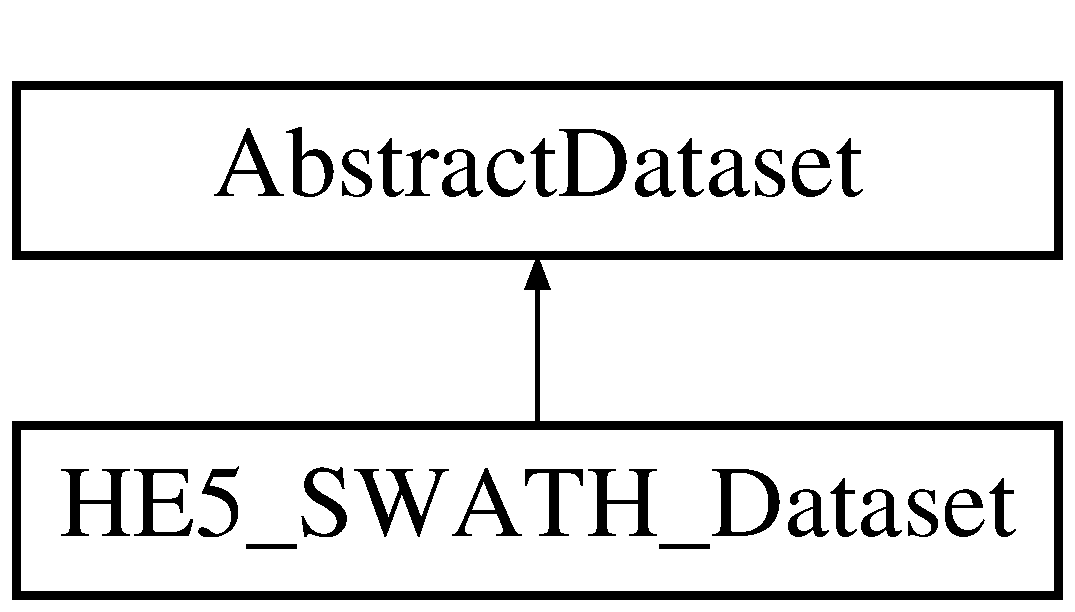
\includegraphics[height=2.000000cm]{classHE5__SWATH__Dataset}
\end{center}
\end{figure}
\subsection*{Public Member Functions}
\begin{DoxyCompactItemize}
\item 
virtual CPLErr \hyperlink{classHE5__SWATH__Dataset_a77dcaecf2d402d69eb3ba0a21536e43e}{SetGeoTransform} ()
\begin{DoxyCompactList}\small\item\em Set the affine GeoTransform matrix for a HDF-\/EOS5 Swath coverage. \end{DoxyCompactList}\item 
virtual CPLErr \hyperlink{classHE5__SWATH__Dataset_a59d87c150c064547f4a9fe4aaa1215b0}{SetMetaDataList} (GDALDataset $\ast$)
\begin{DoxyCompactList}\small\item\em Set the metadata list for this coverage. \end{DoxyCompactList}\item 
virtual CPLErr \hyperlink{classHE5__SWATH__Dataset_a28eeb972e11c417dfef63d96f950318d}{SetNativeCRS} ()
\begin{DoxyCompactList}\small\item\em Set the Native CRS for a HDF-\/EOS Swath dataset. \end{DoxyCompactList}\item 
virtual CPLErr \hyperlink{classHE5__SWATH__Dataset_a549c0943284f1bb4dada2aa5cb8e1f80}{SetGDALDataset} (const int isSimple=0)
\begin{DoxyCompactList}\small\item\em Set the GDALDataset object to HDF-\/EOS5 Swath dataset. \end{DoxyCompactList}\item 
virtual CPLErr \hyperlink{classHE5__SWATH__Dataset_a2dabd5794784f3accdd3e70b0b00ea20}{InitialDataset} (const int isSimple=0)
\begin{DoxyCompactList}\small\item\em Initialize the HDF-\/EOS Swath dataset . \end{DoxyCompactList}\item 
\hyperlink{classHE5__SWATH__Dataset_a4ef63a16c0d5e7dea64f88596584237a}{HE5\_\-SWATH\_\-Dataset} (const string \&id, vector$<$ int $>$ \&rBandList)
\begin{DoxyCompactList}\small\item\em Create an HDF-\/EOS Swath dataset object. \end{DoxyCompactList}\item 
virtual \hyperlink{classHE5__SWATH__Dataset_a856d3c221910b12ae765f2e204c3da45}{$\sim$HE5\_\-SWATH\_\-Dataset} ()
\begin{DoxyCompactList}\small\item\em Destroy an open \hyperlink{classHE5__SWATH__Dataset}{HE5\_\-SWATH\_\-Dataset} object. \end{DoxyCompactList}\item 
virtual int \hyperlink{classHE5__SWATH__Dataset_ae942b004815ec68daa146803825d4173}{GetImageXSize} ()
\begin{DoxyCompactList}\small\item\em Fetch coverage width in pixels. \end{DoxyCompactList}\item 
virtual int \hyperlink{classHE5__SWATH__Dataset_a21bc65038425406fc262c9d430a087ee}{GetImageYSize} ()
\begin{DoxyCompactList}\small\item\em Fetch coverage height in pixels. \end{DoxyCompactList}\end{DoxyCompactItemize}
\subsection*{Protected Attributes}
\begin{DoxyCompactItemize}
\item 
\hypertarget{classHE5__SWATH__Dataset_aa36e85f841155a0da9bba0a54f0349f2}{
int {\bfseries mi\_\-RectifiedImageXSize}}
\label{classHE5__SWATH__Dataset_aa36e85f841155a0da9bba0a54f0349f2}

\item 
\hypertarget{classHE5__SWATH__Dataset_a6126339d82bd638b7b869ad4534a760d}{
int {\bfseries mi\_\-RectifiedImageYSize}}
\label{classHE5__SWATH__Dataset_a6126339d82bd638b7b869ad4534a760d}

\end{DoxyCompactItemize}


\subsection{Detailed Description}
\hyperlink{classHE5__SWATH__Dataset}{HE5\_\-SWATH\_\-Dataset} is a subclass of \hyperlink{classAbstractDataset}{AbstractDataset}, used to process HDF-\/EOS5 Swath coverage. 

HDF-\/EOS is a software library designed to support NASA Earth Observing System (EOS) science data. HDF is the Hierarchical Data Format developed by the National Center for Supercomputing Applications. Specific data structures which are containers for science data are: Grid, Point, Zonal Average and Swath. These data structures are constructed from standard HDF data objects, using EOS conventions, through the use of a software library. A key feature of HDF-\/EOS is a standard prescription for associating geolocation data with science data through internal structural metadata. The relationship between geolocation and science data is transparent to the end-\/user. Instrument and data type-\/independent services, such as subsetting by geolocation, can be applied to files across a wide variety of data products through the same library interface.

Aura data products are mostly in the new HDF-\/EOS5 file format (level 2 and 3), however there are some products which are not (level 1 OMI is in the old HDF-\/EOS2.x, and level 1 MLS is in plain HDF5).

\hyperlink{classHE5__SWATH__Dataset}{HE5\_\-SWATH\_\-Dataset} is a subclass of \hyperlink{classAbstractDataset}{AbstractDataset}, which is used to process Aura Swath products collection, such as OMI OMDOAO3 data.

Sample data could be downloaded from the following link: \href{ftp://aurapar2u.ecs.nasa.gov/data/s4pa///Aura_OMI_Level2/OMDOAO3.003//2011/211/OMI-Aura_L2-OMDOAO3_2011m0730t0925-o37442_v003-2011m0730t151910.he5}{\tt OMI-\/Aura\_\-L2-\/OMDOAO3\_\-2011m0730t0925-\/o37442\_\-v003-\/2011m0730t151910.he5} 

\subsection{Constructor \& Destructor Documentation}
\hypertarget{classHE5__SWATH__Dataset_a4ef63a16c0d5e7dea64f88596584237a}{
\index{HE5\_\-SWATH\_\-Dataset@{HE5\_\-SWATH\_\-Dataset}!HE5\_\-SWATH\_\-Dataset@{HE5\_\-SWATH\_\-Dataset}}
\index{HE5\_\-SWATH\_\-Dataset@{HE5\_\-SWATH\_\-Dataset}!HE5_SWATH_Dataset@{HE5\_\-SWATH\_\-Dataset}}
\subsubsection[{HE5\_\-SWATH\_\-Dataset}]{\setlength{\rightskip}{0pt plus 5cm}HE5\_\-SWATH\_\-Dataset::HE5\_\-SWATH\_\-Dataset (
\begin{DoxyParamCaption}
\item[{const string \&}]{id, }
\item[{vector$<$ int $>$ \&}]{rBandList}
\end{DoxyParamCaption}
)}}
\label{classHE5__SWATH__Dataset_a4ef63a16c0d5e7dea64f88596584237a}


Create an HDF-\/EOS Swath dataset object. 

This is the accepted method of creating a \hyperlink{classHE5__SWATH__Dataset}{HE5\_\-SWATH\_\-Dataset} dataset and allocating all resources associated with it.


\begin{DoxyParams}{Parameters}
{\em id} & The coverage identifier.\\
\hline
{\em rBandList} & The field list selected for this coverage. For HDF-\/EOS5 Swath data, the user may choose multiple range and execute range subset operation.\\
\hline
\end{DoxyParams}
\begin{DoxyReturn}{Returns}
A \hyperlink{classHE5__SWATH__Dataset}{HE5\_\-SWATH\_\-Dataset} object. 
\end{DoxyReturn}
\hypertarget{classHE5__SWATH__Dataset_a856d3c221910b12ae765f2e204c3da45}{
\index{HE5\_\-SWATH\_\-Dataset@{HE5\_\-SWATH\_\-Dataset}!$\sim$HE5\_\-SWATH\_\-Dataset@{$\sim$HE5\_\-SWATH\_\-Dataset}}
\index{$\sim$HE5\_\-SWATH\_\-Dataset@{$\sim$HE5\_\-SWATH\_\-Dataset}!HE5_SWATH_Dataset@{HE5\_\-SWATH\_\-Dataset}}
\subsubsection[{$\sim$HE5\_\-SWATH\_\-Dataset}]{\setlength{\rightskip}{0pt plus 5cm}HE5\_\-SWATH\_\-Dataset::$\sim$HE5\_\-SWATH\_\-Dataset (
\begin{DoxyParamCaption}
{}
\end{DoxyParamCaption}
)\hspace{0.3cm}{\ttfamily  \mbox{[}virtual\mbox{]}}}}
\label{classHE5__SWATH__Dataset_a856d3c221910b12ae765f2e204c3da45}


Destroy an open \hyperlink{classHE5__SWATH__Dataset}{HE5\_\-SWATH\_\-Dataset} object. 

This is the accepted method of closing a \hyperlink{classHE5__SWATH__Dataset}{HE5\_\-SWATH\_\-Dataset} dataset and deallocating all resources associated with it. 

\subsection{Member Function Documentation}
\hypertarget{classHE5__SWATH__Dataset_ae942b004815ec68daa146803825d4173}{
\index{HE5\_\-SWATH\_\-Dataset@{HE5\_\-SWATH\_\-Dataset}!GetImageXSize@{GetImageXSize}}
\index{GetImageXSize@{GetImageXSize}!HE5_SWATH_Dataset@{HE5\_\-SWATH\_\-Dataset}}
\subsubsection[{GetImageXSize}]{\setlength{\rightskip}{0pt plus 5cm}virtual int HE5\_\-SWATH\_\-Dataset::GetImageXSize (
\begin{DoxyParamCaption}
{}
\end{DoxyParamCaption}
)\hspace{0.3cm}{\ttfamily  \mbox{[}inline, virtual\mbox{]}}}}
\label{classHE5__SWATH__Dataset_ae942b004815ec68daa146803825d4173}


Fetch coverage width in pixels. 

The method will return the width of coverage in pixels. GDAL API GetRasterXSize() will be called to generate the width value.

\begin{DoxyReturn}{Returns}
the width in pixels of raster bands in this coverage. 
\end{DoxyReturn}


Reimplemented from \hyperlink{classAbstractDataset_a950e120c5a1e9fa06ee5b02ed4fc6c42}{AbstractDataset}.

\hypertarget{classHE5__SWATH__Dataset_a21bc65038425406fc262c9d430a087ee}{
\index{HE5\_\-SWATH\_\-Dataset@{HE5\_\-SWATH\_\-Dataset}!GetImageYSize@{GetImageYSize}}
\index{GetImageYSize@{GetImageYSize}!HE5_SWATH_Dataset@{HE5\_\-SWATH\_\-Dataset}}
\subsubsection[{GetImageYSize}]{\setlength{\rightskip}{0pt plus 5cm}virtual int HE5\_\-SWATH\_\-Dataset::GetImageYSize (
\begin{DoxyParamCaption}
{}
\end{DoxyParamCaption}
)\hspace{0.3cm}{\ttfamily  \mbox{[}inline, virtual\mbox{]}}}}
\label{classHE5__SWATH__Dataset_a21bc65038425406fc262c9d430a087ee}


Fetch coverage height in pixels. 

The method will return the height of coverage in pixels. GDAL API GetRasterYSize() will be called to generate the height value.

\begin{DoxyReturn}{Returns}
the height in pixels of raster bands in this coverage. 
\end{DoxyReturn}


Reimplemented from \hyperlink{classAbstractDataset_a4f7ceb09ad968d28a5282c7652fb6975}{AbstractDataset}.

\hypertarget{classHE5__SWATH__Dataset_a2dabd5794784f3accdd3e70b0b00ea20}{
\index{HE5\_\-SWATH\_\-Dataset@{HE5\_\-SWATH\_\-Dataset}!InitialDataset@{InitialDataset}}
\index{InitialDataset@{InitialDataset}!HE5_SWATH_Dataset@{HE5\_\-SWATH\_\-Dataset}}
\subsubsection[{InitialDataset}]{\setlength{\rightskip}{0pt plus 5cm}CPLErr HE5\_\-SWATH\_\-Dataset::InitialDataset (
\begin{DoxyParamCaption}
\item[{const int}]{isSimple = {\ttfamily 0}}
\end{DoxyParamCaption}
)\hspace{0.3cm}{\ttfamily  \mbox{[}virtual\mbox{]}}}}
\label{classHE5__SWATH__Dataset_a2dabd5794784f3accdd3e70b0b00ea20}


Initialize the HDF-\/EOS Swath dataset . 

This method is the implementation for initializing a HDF-\/EOS Swath dataset. Within this method, \hyperlink{classHE5__SWATH__Dataset_a28eeb972e11c417dfef63d96f950318d}{SetNativeCRS()}, \hyperlink{classHE5__SWATH__Dataset_a77dcaecf2d402d69eb3ba0a21536e43e}{SetGeoTransform()} and \hyperlink{classHE5__SWATH__Dataset_a549c0943284f1bb4dada2aa5cb8e1f80}{SetGDALDataset()} will be called to initialize an HDF-\/EOS Swath dataset. The coverage type of HDF-\/EOS Swath data is set to \char`\"{}ReferenceableDataset\char`\"{}.


\begin{DoxyParams}{Parameters}
{\em isSimple} & the WCS request type. When user executing a DescribeCoverage request, isSimple is set to 1, and for GetCoverage, is set to 0.\\
\hline
\end{DoxyParams}
\begin{DoxyReturn}{Returns}
CE\_\-None on success or CE\_\-Failure on failure. 
\end{DoxyReturn}


Reimplemented from \hyperlink{classAbstractDataset_a45924895c6bf26c7f75d503b8f6e388a}{AbstractDataset}.

\hypertarget{classHE5__SWATH__Dataset_a549c0943284f1bb4dada2aa5cb8e1f80}{
\index{HE5\_\-SWATH\_\-Dataset@{HE5\_\-SWATH\_\-Dataset}!SetGDALDataset@{SetGDALDataset}}
\index{SetGDALDataset@{SetGDALDataset}!HE5_SWATH_Dataset@{HE5\_\-SWATH\_\-Dataset}}
\subsubsection[{SetGDALDataset}]{\setlength{\rightskip}{0pt plus 5cm}CPLErr HE5\_\-SWATH\_\-Dataset::SetGDALDataset (
\begin{DoxyParamCaption}
\item[{const int}]{isSimple = {\ttfamily 0}}
\end{DoxyParamCaption}
)\hspace{0.3cm}{\ttfamily  \mbox{[}virtual\mbox{]}}}}
\label{classHE5__SWATH__Dataset_a549c0943284f1bb4dada2aa5cb8e1f80}


Set the GDALDataset object to HDF-\/EOS5 Swath dataset. 

This method is used to set the HDF-\/EOS5 Swath dataset.


\begin{DoxyParams}{Parameters}
{\em isSimple} & the WCS request type. When user executing a DescribeCoverage request, isSimple is set to 1, and for GetCoverage, is set to 0.\\
\hline
\end{DoxyParams}
\begin{DoxyReturn}{Returns}
CE\_\-None on success or CE\_\-Failure on failure. 
\end{DoxyReturn}


Reimplemented from \hyperlink{classAbstractDataset_a93bd80bfa48ad45ea53599f289406287}{AbstractDataset}.

\hypertarget{classHE5__SWATH__Dataset_a77dcaecf2d402d69eb3ba0a21536e43e}{
\index{HE5\_\-SWATH\_\-Dataset@{HE5\_\-SWATH\_\-Dataset}!SetGeoTransform@{SetGeoTransform}}
\index{SetGeoTransform@{SetGeoTransform}!HE5_SWATH_Dataset@{HE5\_\-SWATH\_\-Dataset}}
\subsubsection[{SetGeoTransform}]{\setlength{\rightskip}{0pt plus 5cm}CPLErr HE5\_\-SWATH\_\-Dataset::SetGeoTransform (
\begin{DoxyParamCaption}
{}
\end{DoxyParamCaption}
)\hspace{0.3cm}{\ttfamily  \mbox{[}virtual\mbox{]}}}}
\label{classHE5__SWATH__Dataset_a77dcaecf2d402d69eb3ba0a21536e43e}


Set the affine GeoTransform matrix for a HDF-\/EOS5 Swath coverage. 

The method will set a GeoTransform matrix for a HDF-\/EOS5 Swath coverage by parsing and analyzing the metadata of HDF-\/EOS5 Swath data granule. If granule metadata do not include bounding box extent, GDAL\_\-GCP will be used to deduce the bounding box and set the GeoTransform accordingly.

\begin{DoxyReturn}{Returns}
CE\_\-None on success or CE\_\-Failure on failure. 
\end{DoxyReturn}


Reimplemented from \hyperlink{classAbstractDataset_a1d79fc347de75acd57b18c80b9614369}{AbstractDataset}.

\hypertarget{classHE5__SWATH__Dataset_a59d87c150c064547f4a9fe4aaa1215b0}{
\index{HE5\_\-SWATH\_\-Dataset@{HE5\_\-SWATH\_\-Dataset}!SetMetaDataList@{SetMetaDataList}}
\index{SetMetaDataList@{SetMetaDataList}!HE5_SWATH_Dataset@{HE5\_\-SWATH\_\-Dataset}}
\subsubsection[{SetMetaDataList}]{\setlength{\rightskip}{0pt plus 5cm}CPLErr HE5\_\-SWATH\_\-Dataset::SetMetaDataList (
\begin{DoxyParamCaption}
\item[{GDALDataset $\ast$}]{hSrcDS}
\end{DoxyParamCaption}
)\hspace{0.3cm}{\ttfamily  \mbox{[}virtual\mbox{]}}}}
\label{classHE5__SWATH__Dataset_a59d87c150c064547f4a9fe4aaa1215b0}


Set the metadata list for this coverage. 

The method will set the metadata list for the coverage based on its corresponding GDALDataset object.


\begin{DoxyParams}{Parameters}
{\em hSrc} & the GDALDataset object corresponding to coverage.\\
\hline
\end{DoxyParams}
\begin{DoxyReturn}{Returns}
CE\_\-None on success or CE\_\-Failure on failure. 
\end{DoxyReturn}


Reimplemented from \hyperlink{classAbstractDataset_af3f0b55b14f660b79751bf88489a2c10}{AbstractDataset}.

\hypertarget{classHE5__SWATH__Dataset_a28eeb972e11c417dfef63d96f950318d}{
\index{HE5\_\-SWATH\_\-Dataset@{HE5\_\-SWATH\_\-Dataset}!SetNativeCRS@{SetNativeCRS}}
\index{SetNativeCRS@{SetNativeCRS}!HE5_SWATH_Dataset@{HE5\_\-SWATH\_\-Dataset}}
\subsubsection[{SetNativeCRS}]{\setlength{\rightskip}{0pt plus 5cm}CPLErr HE5\_\-SWATH\_\-Dataset::SetNativeCRS (
\begin{DoxyParamCaption}
{}
\end{DoxyParamCaption}
)\hspace{0.3cm}{\ttfamily  \mbox{[}virtual\mbox{]}}}}
\label{classHE5__SWATH__Dataset_a28eeb972e11c417dfef63d96f950318d}


Set the Native CRS for a HDF-\/EOS Swath dataset. 

The method will set the CRS for a HDF-\/EOS5 Swath dataset as an native CRS. Since the coordinates recorded in HDF-\/EOS Swath granule belong to geographic CRS, EPSG:4326 CRS are assigned to HDF-\/EOS Swath dataset.

\begin{DoxyReturn}{Returns}
CE\_\-None on success or CE\_\-Failure on failure. 
\end{DoxyReturn}


Reimplemented from \hyperlink{classAbstractDataset_acfac922d16e5edf51066169bd6ff28ec}{AbstractDataset}.



The documentation for this class was generated from the following files:\begin{DoxyCompactItemize}
\item 
HE5\_\-SWATH\_\-Dataset.h\item 
HE5\_\-SWATH\_\-Dataset.cpp\end{DoxyCompactItemize}

\hypertarget{classKVP}{
\section{KVP Class Reference}
\label{classKVP}\index{KVP@{KVP}}
}
\subsection*{Public Member Functions}
\begin{DoxyCompactItemize}
\item 
\hypertarget{classKVP_a2ec7fe8668a701defe0791c753c68a25}{
\hyperlink{classKVP}{KVP} \& {\bfseries operator=} (const \hyperlink{classKVP}{KVP} \&id)}
\label{classKVP_a2ec7fe8668a701defe0791c753c68a25}

\item 
\hypertarget{classKVP_ada2383a53ee54e47576d9487891e7a88}{
\hyperlink{classKVP}{KVP} \& {\bfseries operator=} (const \hyperlink{classKVP}{KVP} $\ast$pid)}
\label{classKVP_ada2383a53ee54e47576d9487891e7a88}

\item 
\hypertarget{classKVP_a1b5f74b36968db8602ac001040f9faa4}{
{\bfseries KVP} (string n, string v)}
\label{classKVP_a1b5f74b36968db8602ac001040f9faa4}

\item 
\hyperlink{classKVP_a2b7de3a265f04ab40c0ba73b72cb4de4}{KVP} (string namevaluepair)
\begin{DoxyCompactList}\small\item\em Constructor for \hyperlink{classKVP}{KVP}. \end{DoxyCompactList}\end{DoxyCompactItemize}
\subsection*{Public Attributes}
\begin{DoxyCompactItemize}
\item 
\hypertarget{classKVP_ac95b4cb75a07f639baa8b58f93dbcecf}{
string {\bfseries name}}
\label{classKVP_ac95b4cb75a07f639baa8b58f93dbcecf}

\item 
\hypertarget{classKVP_a43bbe2a101f930e2dafc8542629194a4}{
string {\bfseries value}}
\label{classKVP_a43bbe2a101f930e2dafc8542629194a4}

\end{DoxyCompactItemize}


\subsection{Constructor \& Destructor Documentation}
\hypertarget{classKVP_a2b7de3a265f04ab40c0ba73b72cb4de4}{
\index{KVP@{KVP}!KVP@{KVP}}
\index{KVP@{KVP}!KVP@{KVP}}
\subsubsection[{KVP}]{\setlength{\rightskip}{0pt plus 5cm}KVP::KVP (
\begin{DoxyParamCaption}
\item[{string}]{namevaluepair}
\end{DoxyParamCaption}
)}}
\label{classKVP_a2b7de3a265f04ab40c0ba73b72cb4de4}


Constructor for \hyperlink{classKVP}{KVP}. 


\begin{DoxyParams}{Parameters}
{\em namevaluepair} & The key-\/value pair. \\
\hline
\end{DoxyParams}


The documentation for this class was generated from the following files:\begin{DoxyCompactItemize}
\item 
wcsUtil.h\item 
wcsUtil.cpp\end{DoxyCompactItemize}

\hypertarget{classKVPsReader}{
\section{KVPsReader Class Reference}
\label{classKVPsReader}\index{KVPsReader@{KVPsReader}}
}
\subsection*{Public Member Functions}
\begin{DoxyCompactItemize}
\item 
\hypertarget{classKVPsReader_a761728641415f8debcab8952ce001832}{
{\bfseries KVPsReader} (const string \&urlStr, const char \&tok)}
\label{classKVPsReader_a761728641415f8debcab8952ce001832}

\item 
\hypertarget{classKVPsReader_a3d8944ec6b9769148bd716ea1ce53266}{
\hyperlink{classKVP}{KVP} \& {\bfseries operator\mbox{[}$\,$\mbox{]}} (const int index)}
\label{classKVPsReader_a3d8944ec6b9769148bd716ea1ce53266}

\item 
\hypertarget{classKVPsReader_a882a6c61810fce311ffdabf98be4f817}{
int {\bfseries size} ()}
\label{classKVPsReader_a882a6c61810fce311ffdabf98be4f817}

\item 
\hypertarget{classKVPsReader_a65d3870e649cb98473a564c0ca92aee0}{
string {\bfseries getValue} (const string \&keyname)}
\label{classKVPsReader_a65d3870e649cb98473a564c0ca92aee0}

\item 
\hypertarget{classKVPsReader_ae7eb8a9e45adec512620513d9cd05d7f}{
string {\bfseries getValue} (const string \&keyname, const string \&defaultvalue)}
\label{classKVPsReader_ae7eb8a9e45adec512620513d9cd05d7f}

\item 
\hypertarget{classKVPsReader_a3e9bb781a8d88bd0ac15dd1f88329dba}{
vector$<$ string $>$ {\bfseries getValues} (const string \&keyname)}
\label{classKVPsReader_a3e9bb781a8d88bd0ac15dd1f88329dba}

\end{DoxyCompactItemize}
\subsection*{Protected Attributes}
\begin{DoxyCompactItemize}
\item 
\hypertarget{classKVPsReader_aa1500de3a6435e175d469838b44a6ce5}{
vector$<$ \hyperlink{classKVP}{KVP} $>$ {\bfseries m\_\-kvps}}
\label{classKVPsReader_aa1500de3a6435e175d469838b44a6ce5}

\end{DoxyCompactItemize}


The documentation for this class was generated from the following files:\begin{DoxyCompactItemize}
\item 
wcsUtil.h\item 
wcsUtil.cpp\end{DoxyCompactItemize}

\hypertarget{classMy2DPoint}{
\section{My2DPoint Class Reference}
\label{classMy2DPoint}\index{My2DPoint@{My2DPoint}}
}


{\ttfamily \#include \char`\"{}BoundingBox.h\char`\"{}}

\subsection*{Public Member Functions}
\begin{DoxyCompactItemize}
\item 
\hypertarget{classMy2DPoint_a625024d3e1ca0ec8a40479e3ecd91f62}{
{\bfseries My2DPoint} (const double \&xx, const double \&yy)}
\label{classMy2DPoint_a625024d3e1ca0ec8a40479e3ecd91f62}

\item 
\hypertarget{classMy2DPoint_ab07e4cbc4c2880d3eeb8286292f7b8ef}{
{\bfseries My2DPoint} (const \hyperlink{classMy2DPoint}{My2DPoint} \&p)}
\label{classMy2DPoint_ab07e4cbc4c2880d3eeb8286292f7b8ef}

\item 
\hypertarget{classMy2DPoint_af1e5b2795ecad7d9b198db79dd88d2b7}{
\hyperlink{classMy2DPoint}{My2DPoint} \& {\bfseries operator=} (const \hyperlink{classMy2DPoint}{My2DPoint} \&p)}
\label{classMy2DPoint_af1e5b2795ecad7d9b198db79dd88d2b7}

\end{DoxyCompactItemize}
\subsection*{Public Attributes}
\begin{DoxyCompactItemize}
\item 
\hypertarget{classMy2DPoint_ab35881833d7e86c44789e08dd1873e69}{
double {\bfseries mi\_\-X}}
\label{classMy2DPoint_ab35881833d7e86c44789e08dd1873e69}

\item 
\hypertarget{classMy2DPoint_a2118443cacdcd7b85f6ef3a1e57fddcc}{
double {\bfseries mi\_\-Y}}
\label{classMy2DPoint_a2118443cacdcd7b85f6ef3a1e57fddcc}

\end{DoxyCompactItemize}


\subsection{Detailed Description}
\hyperlink{classMy2DPoint}{My2DPoint} class is used to store the point coordinates. 

The documentation for this class was generated from the following files:\begin{DoxyCompactItemize}
\item 
BoundingBox.h\item 
BoundingBox.cpp\end{DoxyCompactItemize}

\hypertarget{classNC__GOES__Dataset}{
\section{NC\_\-GOES\_\-Dataset Class Reference}
\label{classNC__GOES__Dataset}\index{NC\_\-GOES\_\-Dataset@{NC\_\-GOES\_\-Dataset}}
}


\hyperlink{classNC__GOES__Dataset}{NC\_\-GOES\_\-Dataset} is a subclass of \hyperlink{classAbstractDataset}{AbstractDataset}, used to process NOAA GOES data.  




{\ttfamily \#include \char`\"{}NC\_\-GOES\_\-Dataset.h\char`\"{}}

Inheritance diagram for NC\_\-GOES\_\-Dataset:\begin{figure}[H]
\begin{center}
\leavevmode
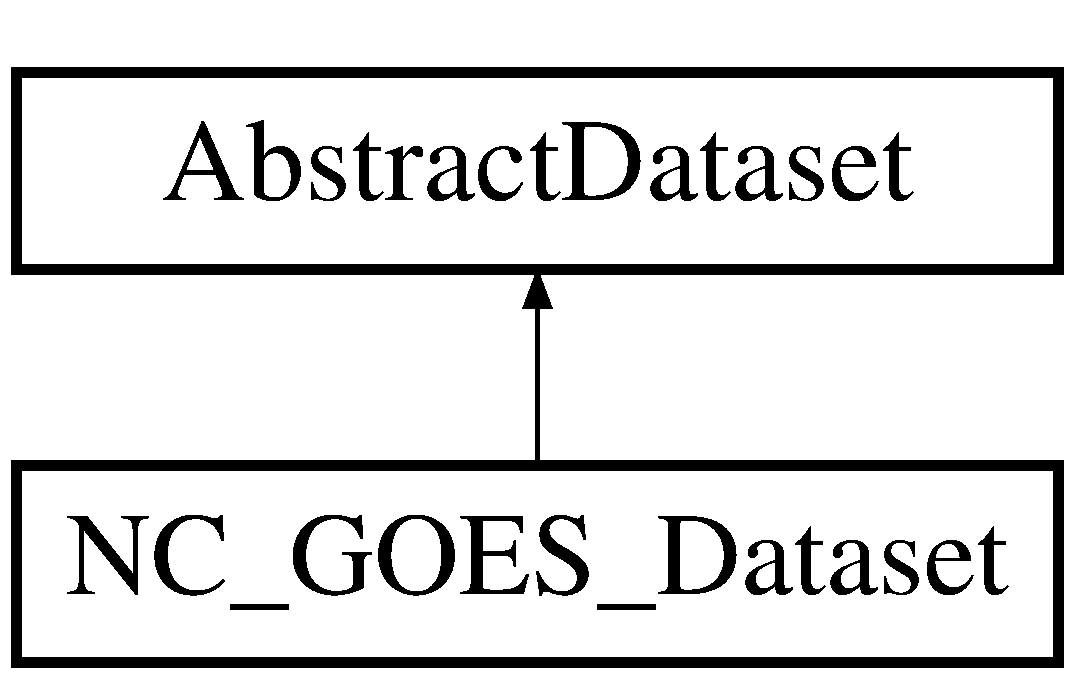
\includegraphics[height=2.000000cm]{classNC__GOES__Dataset}
\end{center}
\end{figure}
\subsection*{Public Member Functions}
\begin{DoxyCompactItemize}
\item 
CPLErr \hyperlink{classNC__GOES__Dataset_afc729a63579f05daca3ebda085762026}{SetGCPGeoRef4VRTDataset} (GDALDataset $\ast$)
\begin{DoxyCompactList}\small\item\em Set the GCP array for the VRT dataset. \end{DoxyCompactList}\item 
CPLErr \hyperlink{classNC__GOES__Dataset_a2834229e8688e7ba0a8a135d8620d9a4}{SetGeoBBoxAndGCPs} (GDALDataset $\ast$hSrcDS)
\begin{DoxyCompactList}\small\item\em Set the native geographical bounding box and GCP array for a GOES data. \end{DoxyCompactList}\item 
CPLErr \hyperlink{classNC__GOES__Dataset_ae413433045908f2bd7d75a1c3c31fb03}{RectifyGOESDataSet} ()
\begin{DoxyCompactList}\small\item\em Convert the GOES dataset from satellite CRS project to grid CRS. \end{DoxyCompactList}\item 
\hypertarget{classNC__GOES__Dataset_ae16362490482905d96a92f6f09763601}{
CPLErr {\bfseries setResampleStandard} (GDALDataset $\ast$hSrcDS, int \&xRSValue, int \&yRSValue)}
\label{classNC__GOES__Dataset_ae16362490482905d96a92f6f09763601}

\item 
\hypertarget{classNC__GOES__Dataset_ae3546f1308a32fa402214b71d386a875}{
int {\bfseries isValidLatitude} (const double \&lat)}
\label{classNC__GOES__Dataset_ae3546f1308a32fa402214b71d386a875}

\item 
\hypertarget{classNC__GOES__Dataset_a5a32111ae54572d57812acb65cbce762}{
int {\bfseries isValidLongitude} (const double \&lon)}
\label{classNC__GOES__Dataset_a5a32111ae54572d57812acb65cbce762}

\item 
virtual CPLErr \hyperlink{classNC__GOES__Dataset_ada85679c832ad2ff971d6291ccf9b8f8}{SetGeoTransform} ()
\begin{DoxyCompactList}\small\item\em Set the affine GeoTransform matrix for a GOES data. \end{DoxyCompactList}\item 
virtual CPLErr \hyperlink{classNC__GOES__Dataset_ae5e798ca0bb105513a80fcdb0b5cf9d8}{SetMetaDataList} (GDALDataset $\ast$hSrcDS)
\begin{DoxyCompactList}\small\item\em Set the metadata list for this coverage. \end{DoxyCompactList}\item 
virtual CPLErr \hyperlink{classNC__GOES__Dataset_abc062e894fdf1731f5b258091ffcc5ea}{SetNativeCRS} ()
\begin{DoxyCompactList}\small\item\em Set the Native CRS for a GOES dataset. \end{DoxyCompactList}\item 
virtual CPLErr \hyperlink{classNC__GOES__Dataset_a2ec90aa02b68185edbdd1fa00727ed10}{SetGDALDataset} (const int isSimple=0)
\begin{DoxyCompactList}\small\item\em Set the GDALDataset object to GOES Imager and Sounder dataset. \end{DoxyCompactList}\item 
virtual CPLErr \hyperlink{classNC__GOES__Dataset_a128b874278c0ad4dd093baf22bf8d23f}{InitialDataset} (const int isSimple=0)
\begin{DoxyCompactList}\small\item\em Initialize the GOES dataset with NetCDF format. \end{DoxyCompactList}\item 
virtual CPLErr \hyperlink{classNC__GOES__Dataset_a5d2fa4d635bae04a1b488b1917dd7ab3}{GetGeoMinMax} (double geoMinMax\mbox{[}$\,$\mbox{]})
\begin{DoxyCompactList}\small\item\em Get the min/max coordinates of laitutude and longitude. \end{DoxyCompactList}\item 
\hyperlink{classNC__GOES__Dataset_a481c60e90f61c2ff2fa82dfe78eed0ba}{NC\_\-GOES\_\-Dataset} (const string \&id, vector$<$ int $>$ \&rBandList)
\begin{DoxyCompactList}\small\item\em Create an \hyperlink{classNC__GOES__Dataset}{NC\_\-GOES\_\-Dataset} object. \end{DoxyCompactList}\item 
virtual \hyperlink{classNC__GOES__Dataset_a89368fa51f93a6eb45529d4c484cee64}{$\sim$NC\_\-GOES\_\-Dataset} ()
\begin{DoxyCompactList}\small\item\em Destroy an open \hyperlink{classNC__GOES__Dataset}{NC\_\-GOES\_\-Dataset} object. \end{DoxyCompactList}\end{DoxyCompactItemize}
\subsection*{Protected Attributes}
\begin{DoxyCompactItemize}
\item 
\hypertarget{classNC__GOES__Dataset_af4bb45c48b0138a9e78c9649219232ec}{
string {\bfseries m\_\-ncLatDataSetName}}
\label{classNC__GOES__Dataset_af4bb45c48b0138a9e78c9649219232ec}

\item 
\hypertarget{classNC__GOES__Dataset_a422d930b4d65dead03d2c3bdf214042c}{
string {\bfseries m\_\-ncLonDataSetName}}
\label{classNC__GOES__Dataset_a422d930b4d65dead03d2c3bdf214042c}

\item 
\hypertarget{classNC__GOES__Dataset_aa59afbdd42da66b22ce325860ac09b8f}{
string {\bfseries m\_\-ncCoverageIDName}}
\label{classNC__GOES__Dataset_aa59afbdd42da66b22ce325860ac09b8f}

\item 
\hypertarget{classNC__GOES__Dataset_a5dd4cda3caa1dc0f311a4d3abe2430bd}{
int {\bfseries mi\_\-RectifiedImageXSize}}
\label{classNC__GOES__Dataset_a5dd4cda3caa1dc0f311a4d3abe2430bd}

\item 
\hypertarget{classNC__GOES__Dataset_a8182e9221e03787515fc6dc7a4a0a3b8}{
int {\bfseries mi\_\-RectifiedImageYSize}}
\label{classNC__GOES__Dataset_a8182e9221e03787515fc6dc7a4a0a3b8}

\item 
\hypertarget{classNC__GOES__Dataset_a0b59f3c7174c3459b95bf182563f822a}{
int {\bfseries mi\_\-GoesSrcImageXSize}}
\label{classNC__GOES__Dataset_a0b59f3c7174c3459b95bf182563f822a}

\item 
\hypertarget{classNC__GOES__Dataset_a488313f9fd495daeafea1db6924174b5}{
int {\bfseries mi\_\-GoesSrcImageYSize}}
\label{classNC__GOES__Dataset_a488313f9fd495daeafea1db6924174b5}

\item 
\hypertarget{classNC__GOES__Dataset_a15b98e620c10526415c7bf1a3deb0b89}{
double {\bfseries mb\_\-LatLonBBox} \mbox{[}4\mbox{]}}
\label{classNC__GOES__Dataset_a15b98e620c10526415c7bf1a3deb0b89}

\item 
\hypertarget{classNC__GOES__Dataset_a26e7b6a6c1e71e7d07a36e48b802593d}{
double {\bfseries mdSrcGeoMinX}}
\label{classNC__GOES__Dataset_a26e7b6a6c1e71e7d07a36e48b802593d}

\item 
\hypertarget{classNC__GOES__Dataset_a706dc5472f1f32bd949a00d7e6d0ff53}{
double {\bfseries mdSrcGeoMinY}}
\label{classNC__GOES__Dataset_a706dc5472f1f32bd949a00d7e6d0ff53}

\item 
\hypertarget{classNC__GOES__Dataset_a4d953ce0c73a23c4e7de48db31f1c486}{
double {\bfseries mdSrcGeoMaxX}}
\label{classNC__GOES__Dataset_a4d953ce0c73a23c4e7de48db31f1c486}

\item 
\hypertarget{classNC__GOES__Dataset_aea7c01d4ca66cad665f0f3b209b5b430}{
double {\bfseries mdSrcGeoMaxY}}
\label{classNC__GOES__Dataset_aea7c01d4ca66cad665f0f3b209b5b430}

\item 
\hypertarget{classNC__GOES__Dataset_a79fbf36f7e91c498b6d232c63a662be7}{
vector$<$ GDAL\_\-GCP $>$ {\bfseries m\_\-gdalGCPs}}
\label{classNC__GOES__Dataset_a79fbf36f7e91c498b6d232c63a662be7}

\end{DoxyCompactItemize}


\subsection{Detailed Description}
\hyperlink{classNC__GOES__Dataset}{NC\_\-GOES\_\-Dataset} is a subclass of \hyperlink{classAbstractDataset}{AbstractDataset}, used to process NOAA GOES data. 

GOES satellites provide the kind of continuous monitoring necessary for intensive data analysis. They circle the Earth in a geosynchronous orbit, which means they orbit the equatorial plane of the Earth at a speed matching the Earth's rotation. This allows them to hover continuously over one position on the surface. The geosynchronous plane is about 35,800 km (22,300 miles) above the Earth, high enough to allow the satellites a full-\/disc view of the Earth. Because they stay above a fixed spot on the surface, they provide a constant vigil for the atmospheric \char`\"{}triggers\char`\"{} for severe weather conditions such as tornadoes, flash floods, hail storms, and hurricanes. When these conditions develop the GOES satellites are able to monitor storm development and track their movements.

GOES satellite imagery is also used to estimate rainfall during the thunderstorms and hurricanes for flash flood warnings, as well as estimates snowfall accumulations and overall extent of snow cover. Such data help meteorologists issue winter storm warnings and spring snow melt advisories. Satellite sensors also detect ice fields and map the movements of sea and lake ice.

For more inforamtion about NOAA GOES data, please access \href{http://www.oso.noaa.gov/GOES/}{\tt http://www.oso.noaa.gov/GOES/}

\hyperlink{classNC__GOES__Dataset}{NC\_\-GOES\_\-Dataset} is a subclass of \hyperlink{classAbstractDataset}{AbstractDataset}, which is used to process GOES Imager and Sounder products. 

\subsection{Constructor \& Destructor Documentation}
\hypertarget{classNC__GOES__Dataset_a481c60e90f61c2ff2fa82dfe78eed0ba}{
\index{NC\_\-GOES\_\-Dataset@{NC\_\-GOES\_\-Dataset}!NC\_\-GOES\_\-Dataset@{NC\_\-GOES\_\-Dataset}}
\index{NC\_\-GOES\_\-Dataset@{NC\_\-GOES\_\-Dataset}!NC_GOES_Dataset@{NC\_\-GOES\_\-Dataset}}
\subsubsection[{NC\_\-GOES\_\-Dataset}]{\setlength{\rightskip}{0pt plus 5cm}NC\_\-GOES\_\-Dataset::NC\_\-GOES\_\-Dataset (
\begin{DoxyParamCaption}
\item[{const string \&}]{id, }
\item[{vector$<$ int $>$ \&}]{rBandList}
\end{DoxyParamCaption}
)}}
\label{classNC__GOES__Dataset_a481c60e90f61c2ff2fa82dfe78eed0ba}


Create an \hyperlink{classNC__GOES__Dataset}{NC\_\-GOES\_\-Dataset} object. 

This is the accepted method of creating a \hyperlink{classNC__GOES__Dataset}{NC\_\-GOES\_\-Dataset} object and allocating all resources associated with it.


\begin{DoxyParams}{Parameters}
{\em id} & The coverage identifier.\\
\hline
{\em rBandList} & The field list selected for this coverage. For TRMM daily data, the user could specify multiple days range in request. Each day is seemed as one field.\\
\hline
\end{DoxyParams}
\begin{DoxyReturn}{Returns}
A \hyperlink{classNC__GOES__Dataset}{NC\_\-GOES\_\-Dataset} object. 
\end{DoxyReturn}
\hypertarget{classNC__GOES__Dataset_a89368fa51f93a6eb45529d4c484cee64}{
\index{NC\_\-GOES\_\-Dataset@{NC\_\-GOES\_\-Dataset}!$\sim$NC\_\-GOES\_\-Dataset@{$\sim$NC\_\-GOES\_\-Dataset}}
\index{$\sim$NC\_\-GOES\_\-Dataset@{$\sim$NC\_\-GOES\_\-Dataset}!NC_GOES_Dataset@{NC\_\-GOES\_\-Dataset}}
\subsubsection[{$\sim$NC\_\-GOES\_\-Dataset}]{\setlength{\rightskip}{0pt plus 5cm}NC\_\-GOES\_\-Dataset::$\sim$NC\_\-GOES\_\-Dataset (
\begin{DoxyParamCaption}
{}
\end{DoxyParamCaption}
)\hspace{0.3cm}{\ttfamily  \mbox{[}virtual\mbox{]}}}}
\label{classNC__GOES__Dataset_a89368fa51f93a6eb45529d4c484cee64}


Destroy an open \hyperlink{classNC__GOES__Dataset}{NC\_\-GOES\_\-Dataset} object. 

This is the accepted method of closing a \hyperlink{classNC__GOES__Dataset}{NC\_\-GOES\_\-Dataset} dataset and deallocating all resources associated with it. 

\subsection{Member Function Documentation}
\hypertarget{classNC__GOES__Dataset_a5d2fa4d635bae04a1b488b1917dd7ab3}{
\index{NC\_\-GOES\_\-Dataset@{NC\_\-GOES\_\-Dataset}!GetGeoMinMax@{GetGeoMinMax}}
\index{GetGeoMinMax@{GetGeoMinMax}!NC_GOES_Dataset@{NC\_\-GOES\_\-Dataset}}
\subsubsection[{GetGeoMinMax}]{\setlength{\rightskip}{0pt plus 5cm}CPLErr NC\_\-GOES\_\-Dataset::GetGeoMinMax (
\begin{DoxyParamCaption}
\item[{double}]{geoMinMax\mbox{[}$\,$\mbox{]}}
\end{DoxyParamCaption}
)\hspace{0.3cm}{\ttfamily  \mbox{[}virtual\mbox{]}}}}
\label{classNC__GOES__Dataset_a5d2fa4d635bae04a1b488b1917dd7ab3}


Get the min/max coordinates of laitutude and longitude. 

The method will fetch the min/max coordinates of laitutude and longitude.


\begin{DoxyParams}{Parameters}
{\em geoMinMax} & an existing four double buffer into which the native geographical bounding box values will be placed.\\
\hline
\end{DoxyParams}
\begin{DoxyReturn}{Returns}
CE\_\-None on success or CE\_\-Failure on failure. 
\end{DoxyReturn}


Reimplemented from \hyperlink{classAbstractDataset_a66a65ce60f813d0ef683919a098b8a98}{AbstractDataset}.

\hypertarget{classNC__GOES__Dataset_a128b874278c0ad4dd093baf22bf8d23f}{
\index{NC\_\-GOES\_\-Dataset@{NC\_\-GOES\_\-Dataset}!InitialDataset@{InitialDataset}}
\index{InitialDataset@{InitialDataset}!NC_GOES_Dataset@{NC\_\-GOES\_\-Dataset}}
\subsubsection[{InitialDataset}]{\setlength{\rightskip}{0pt plus 5cm}CPLErr NC\_\-GOES\_\-Dataset::InitialDataset (
\begin{DoxyParamCaption}
\item[{const int}]{isSimple = {\ttfamily 0}}
\end{DoxyParamCaption}
)\hspace{0.3cm}{\ttfamily  \mbox{[}virtual\mbox{]}}}}
\label{classNC__GOES__Dataset_a128b874278c0ad4dd093baf22bf8d23f}


Initialize the GOES dataset with NetCDF format. 

This method is the implementation for initializing a GOES dataset with NetCDF format. Within this method, \hyperlink{classNC__GOES__Dataset_abc062e894fdf1731f5b258091ffcc5ea}{SetNativeCRS()}, \hyperlink{classNC__GOES__Dataset_ada85679c832ad2ff971d6291ccf9b8f8}{SetGeoTransform()} and \hyperlink{classNC__GOES__Dataset_a2ec90aa02b68185edbdd1fa00727ed10}{SetGDALDataset()} will be called to initialize an GOES dataset.


\begin{DoxyParams}{Parameters}
{\em isSimple} & the WCS request type. When user executing a DescribeCoverage request, isSimple is set to 1, and for GetCoverage, is set to 0.\\
\hline
\end{DoxyParams}
\begin{DoxyReturn}{Returns}
CE\_\-None on success or CE\_\-Failure on failure. 
\end{DoxyReturn}


Reimplemented from \hyperlink{classAbstractDataset_a45924895c6bf26c7f75d503b8f6e388a}{AbstractDataset}.

\hypertarget{classNC__GOES__Dataset_ae413433045908f2bd7d75a1c3c31fb03}{
\index{NC\_\-GOES\_\-Dataset@{NC\_\-GOES\_\-Dataset}!RectifyGOESDataSet@{RectifyGOESDataSet}}
\index{RectifyGOESDataSet@{RectifyGOESDataSet}!NC_GOES_Dataset@{NC\_\-GOES\_\-Dataset}}
\subsubsection[{RectifyGOESDataSet}]{\setlength{\rightskip}{0pt plus 5cm}CPLErr NC\_\-GOES\_\-Dataset::RectifyGOESDataSet (
\begin{DoxyParamCaption}
{}
\end{DoxyParamCaption}
)}}
\label{classNC__GOES__Dataset_ae413433045908f2bd7d75a1c3c31fb03}


Convert the GOES dataset from satellite CRS project to grid CRS. 

The method will convert the GOES dataset from satellite CRS project to grid CRS based on GDAL API GDALReprojectImage;

\begin{DoxyReturn}{Returns}
CE\_\-None on success or CE\_\-Failure on failure. 
\end{DoxyReturn}
\hypertarget{classNC__GOES__Dataset_afc729a63579f05daca3ebda085762026}{
\index{NC\_\-GOES\_\-Dataset@{NC\_\-GOES\_\-Dataset}!SetGCPGeoRef4VRTDataset@{SetGCPGeoRef4VRTDataset}}
\index{SetGCPGeoRef4VRTDataset@{SetGCPGeoRef4VRTDataset}!NC_GOES_Dataset@{NC\_\-GOES\_\-Dataset}}
\subsubsection[{SetGCPGeoRef4VRTDataset}]{\setlength{\rightskip}{0pt plus 5cm}CPLErr NC\_\-GOES\_\-Dataset::SetGCPGeoRef4VRTDataset (
\begin{DoxyParamCaption}
\item[{GDALDataset $\ast$}]{poVDS}
\end{DoxyParamCaption}
)}}
\label{classNC__GOES__Dataset_afc729a63579f05daca3ebda085762026}


Set the GCP array for the VRT dataset. 

This method is used to set the GCP array to created VRT dataset based on GDAL method SetGCPs().


\begin{DoxyParams}{Parameters}
{\em poVDS} & The VRT dataset.\\
\hline
\end{DoxyParams}
\begin{DoxyReturn}{Returns}
CE\_\-None on success or CE\_\-Failure on failure. 
\end{DoxyReturn}
\hypertarget{classNC__GOES__Dataset_a2ec90aa02b68185edbdd1fa00727ed10}{
\index{NC\_\-GOES\_\-Dataset@{NC\_\-GOES\_\-Dataset}!SetGDALDataset@{SetGDALDataset}}
\index{SetGDALDataset@{SetGDALDataset}!NC_GOES_Dataset@{NC\_\-GOES\_\-Dataset}}
\subsubsection[{SetGDALDataset}]{\setlength{\rightskip}{0pt plus 5cm}CPLErr NC\_\-GOES\_\-Dataset::SetGDALDataset (
\begin{DoxyParamCaption}
\item[{const int}]{isSimple = {\ttfamily 0}}
\end{DoxyParamCaption}
)\hspace{0.3cm}{\ttfamily  \mbox{[}virtual\mbox{]}}}}
\label{classNC__GOES__Dataset_a2ec90aa02b68185edbdd1fa00727ed10}


Set the GDALDataset object to GOES Imager and Sounder dataset. 

This method is used to set the GOES Imager and Sounder dataset based on GDAL class VRTDataset.


\begin{DoxyParams}{Parameters}
{\em isSimple} & the WCS request type. When user executing a DescribeCoverage request, isSimple is set to 1, and for GetCoverage, is set to 0.\\
\hline
\end{DoxyParams}
\begin{DoxyReturn}{Returns}
CE\_\-None on success or CE\_\-Failure on failure. 
\end{DoxyReturn}


Reimplemented from \hyperlink{classAbstractDataset_a93bd80bfa48ad45ea53599f289406287}{AbstractDataset}.

\hypertarget{classNC__GOES__Dataset_a2834229e8688e7ba0a8a135d8620d9a4}{
\index{NC\_\-GOES\_\-Dataset@{NC\_\-GOES\_\-Dataset}!SetGeoBBoxAndGCPs@{SetGeoBBoxAndGCPs}}
\index{SetGeoBBoxAndGCPs@{SetGeoBBoxAndGCPs}!NC_GOES_Dataset@{NC\_\-GOES\_\-Dataset}}
\subsubsection[{SetGeoBBoxAndGCPs}]{\setlength{\rightskip}{0pt plus 5cm}CPLErr NC\_\-GOES\_\-Dataset::SetGeoBBoxAndGCPs (
\begin{DoxyParamCaption}
\item[{GDALDataset $\ast$}]{poVDS}
\end{DoxyParamCaption}
)}}
\label{classNC__GOES__Dataset_a2834229e8688e7ba0a8a135d8620d9a4}


Set the native geographical bounding box and GCP array for a GOES data. 

The method will set the native geographical bounding box by comparing the coordinates values existed in longitude and latitude field.


\begin{DoxyParams}{Parameters}
{\em poVDS} & The GDAL dataset returned by calling GDALOpen() method.\\
\hline
\end{DoxyParams}
\begin{DoxyReturn}{Returns}
CE\_\-None on success or CE\_\-Failure on failure. 
\end{DoxyReturn}
\hypertarget{classNC__GOES__Dataset_ada85679c832ad2ff971d6291ccf9b8f8}{
\index{NC\_\-GOES\_\-Dataset@{NC\_\-GOES\_\-Dataset}!SetGeoTransform@{SetGeoTransform}}
\index{SetGeoTransform@{SetGeoTransform}!NC_GOES_Dataset@{NC\_\-GOES\_\-Dataset}}
\subsubsection[{SetGeoTransform}]{\setlength{\rightskip}{0pt plus 5cm}CPLErr NC\_\-GOES\_\-Dataset::SetGeoTransform (
\begin{DoxyParamCaption}
{}
\end{DoxyParamCaption}
)\hspace{0.3cm}{\ttfamily  \mbox{[}virtual\mbox{]}}}}
\label{classNC__GOES__Dataset_ada85679c832ad2ff971d6291ccf9b8f8}


Set the affine GeoTransform matrix for a GOES data. 

The method will set a GeoTransform matrix for a GOES data by parsing the coordinates values existed in longitude and latitude field.

The CRS for the bounding box is EPSG:4326.

\begin{DoxyReturn}{Returns}
CE\_\-None on success or CE\_\-Failure on failure. 
\end{DoxyReturn}


Reimplemented from \hyperlink{classAbstractDataset_a1d79fc347de75acd57b18c80b9614369}{AbstractDataset}.

\hypertarget{classNC__GOES__Dataset_ae5e798ca0bb105513a80fcdb0b5cf9d8}{
\index{NC\_\-GOES\_\-Dataset@{NC\_\-GOES\_\-Dataset}!SetMetaDataList@{SetMetaDataList}}
\index{SetMetaDataList@{SetMetaDataList}!NC_GOES_Dataset@{NC\_\-GOES\_\-Dataset}}
\subsubsection[{SetMetaDataList}]{\setlength{\rightskip}{0pt plus 5cm}CPLErr NC\_\-GOES\_\-Dataset::SetMetaDataList (
\begin{DoxyParamCaption}
\item[{GDALDataset $\ast$}]{hSrcDS}
\end{DoxyParamCaption}
)\hspace{0.3cm}{\ttfamily  \mbox{[}virtual\mbox{]}}}}
\label{classNC__GOES__Dataset_ae5e798ca0bb105513a80fcdb0b5cf9d8}


Set the metadata list for this coverage. 

The method will set the metadata list for the coverage based on its corresponding GDALDataset object.


\begin{DoxyParams}{Parameters}
{\em hSrc} & the GDALDataset object corresponding to coverage.\\
\hline
\end{DoxyParams}
\begin{DoxyReturn}{Returns}
CE\_\-None on success or CE\_\-Failure on failure. 
\end{DoxyReturn}


Reimplemented from \hyperlink{classAbstractDataset_af3f0b55b14f660b79751bf88489a2c10}{AbstractDataset}.

\hypertarget{classNC__GOES__Dataset_abc062e894fdf1731f5b258091ffcc5ea}{
\index{NC\_\-GOES\_\-Dataset@{NC\_\-GOES\_\-Dataset}!SetNativeCRS@{SetNativeCRS}}
\index{SetNativeCRS@{SetNativeCRS}!NC_GOES_Dataset@{NC\_\-GOES\_\-Dataset}}
\subsubsection[{SetNativeCRS}]{\setlength{\rightskip}{0pt plus 5cm}CPLErr NC\_\-GOES\_\-Dataset::SetNativeCRS (
\begin{DoxyParamCaption}
{}
\end{DoxyParamCaption}
)\hspace{0.3cm}{\ttfamily  \mbox{[}virtual\mbox{]}}}}
\label{classNC__GOES__Dataset_abc062e894fdf1731f5b258091ffcc5ea}


Set the Native CRS for a GOES dataset. 

The method will set the CRS for a GOES dataset as an native CRS.

Since the original GOES data adopt satellite CRS to recored its value, like MODIS swath data, each data point has its corresponding latitude and longitude value, those coordinates could be fetched in another two fields.

The native CRS for GOES Imager and Sounder data is assigned to EPSG:4326 if both the latitude and longitude are existed.

\begin{DoxyReturn}{Returns}
CE\_\-None on success or CE\_\-Failure on failure. 
\end{DoxyReturn}


Reimplemented from \hyperlink{classAbstractDataset_acfac922d16e5edf51066169bd6ff28ec}{AbstractDataset}.



The documentation for this class was generated from the following files:\begin{DoxyCompactItemize}
\item 
NC\_\-GOES\_\-Dataset.h\item 
NC\_\-GOES\_\-Dataset.cpp\end{DoxyCompactItemize}

\hypertarget{classS2C}{
\section{S2C Class Reference}
\label{classS2C}\index{S2C@{S2C}}
}
\subsection*{Public Member Functions}
\begin{DoxyCompactItemize}
\item 
\hypertarget{classS2C_a1bc83eb080cbfbe7be081743342a75ca}{
{\bfseries S2C} (string s)}
\label{classS2C_a1bc83eb080cbfbe7be081743342a75ca}

\item 
\hypertarget{classS2C_abbb0cc88f841f21586c6622cb740c65f}{
char $\ast$ {\bfseries c\_\-str} ()}
\label{classS2C_abbb0cc88f841f21586c6622cb740c65f}

\end{DoxyCompactItemize}


The documentation for this class was generated from the following file:\begin{DoxyCompactItemize}
\item 
wcsUtil.h\end{DoxyCompactItemize}

\hypertarget{classStitchedMosaicObject}{
\section{StitchedMosaicObject Class Reference}
\label{classStitchedMosaicObject}\index{StitchedMosaicObject@{StitchedMosaicObject}}
}


\hyperlink{classStitchedMosaicObject}{StitchedMosaicObject} class is used to record stitched mosaic coverage attributes.  




{\ttfamily \#include $<$WCS\_\-T.h$>$}

\subsection*{Public Attributes}
\begin{DoxyCompactItemize}
\item 
\hypertarget{classStitchedMosaicObject_aa5ed2331208efee194b57704ea79d042}{
vector$<$ \hyperlink{classDatasetObject}{DatasetObject} $>$ {\bfseries mv\_\-dataset}}
\label{classStitchedMosaicObject_aa5ed2331208efee194b57704ea79d042}

\item 
\hypertarget{classStitchedMosaicObject_a625fa7902cf715c5bd8df4399beb44ca}{
string {\bfseries m\_\-covName}}
\label{classStitchedMosaicObject_a625fa7902cf715c5bd8df4399beb44ca}

\item 
\hypertarget{classStitchedMosaicObject_a1b723345995e4f4c3f180b02136b6aa2}{
string {\bfseries m\_\-beginTime}}
\label{classStitchedMosaicObject_a1b723345995e4f4c3f180b02136b6aa2}

\item 
\hypertarget{classStitchedMosaicObject_ac3f2f4043f179fdbe3cbeac5002bf2cf}{
string {\bfseries m\_\-endTime}}
\label{classStitchedMosaicObject_ac3f2f4043f179fdbe3cbeac5002bf2cf}

\item 
\hypertarget{classStitchedMosaicObject_a938c2229ff00490cc2404d5b0621dbf2}{
double {\bfseries m\_\-minx}}
\label{classStitchedMosaicObject_a938c2229ff00490cc2404d5b0621dbf2}

\item 
\hypertarget{classStitchedMosaicObject_abf285c40f416556821bae49e73b79910}{
double {\bfseries m\_\-maxx}}
\label{classStitchedMosaicObject_abf285c40f416556821bae49e73b79910}

\item 
\hypertarget{classStitchedMosaicObject_a1a1dc03968ab40a41939835daa8ea154}{
double {\bfseries m\_\-miny}}
\label{classStitchedMosaicObject_a1a1dc03968ab40a41939835daa8ea154}

\item 
\hypertarget{classStitchedMosaicObject_ad472779a00ad7d333f4a5aeaa95c722c}{
double {\bfseries m\_\-maxy}}
\label{classStitchedMosaicObject_ad472779a00ad7d333f4a5aeaa95c722c}

\end{DoxyCompactItemize}


\subsection{Detailed Description}
\hyperlink{classStitchedMosaicObject}{StitchedMosaicObject} class is used to record stitched mosaic coverage attributes. 

The documentation for this class was generated from the following file:\begin{DoxyCompactItemize}
\item 
WCS\_\-T.h\end{DoxyCompactItemize}

\hypertarget{classStringList}{
\section{StringList Class Reference}
\label{classStringList}\index{StringList@{StringList}}
}
\subsection*{Public Member Functions}
\begin{DoxyCompactItemize}
\item 
\hypertarget{classStringList_a0e2782b895540a5d7ccbc3bb2b9defa6}{
\hyperlink{classStringList_a0e2782b895540a5d7ccbc3bb2b9defa6}{StringList} (const string \&sstrings, const char delimiter)}
\label{classStringList_a0e2782b895540a5d7ccbc3bb2b9defa6}

\begin{DoxyCompactList}\small\item\em Constructor for \hyperlink{classStringList}{StringList}. \end{DoxyCompactList}\item 
\hypertarget{classStringList_aab2b9be958fdd8ef37f576bc6950deb6}{
{\bfseries StringList} (const string \&sstrings, const string \&delimiters)}
\label{classStringList_aab2b9be958fdd8ef37f576bc6950deb6}

\item 
\hypertarget{classStringList_ad362163892d7242e8db461dfc7af52f4}{
int {\bfseries indexof} (string qstr)}
\label{classStringList_ad362163892d7242e8db461dfc7af52f4}

\item 
\hypertarget{classStringList_aeec14f49deaaa845deed7886cf7f1d4b}{
void {\bfseries add} (string newstr)}
\label{classStringList_aeec14f49deaaa845deed7886cf7f1d4b}

\item 
\hypertarget{classStringList_a5ad2ccbfc0d55ebd1239af8dfa687abe}{
void {\bfseries clear} ()}
\label{classStringList_a5ad2ccbfc0d55ebd1239af8dfa687abe}

\item 
\hypertarget{classStringList_a7839bcac8a6d8329905dfca91db7894d}{
int {\bfseries size} ()}
\label{classStringList_a7839bcac8a6d8329905dfca91db7894d}

\item 
\hypertarget{classStringList_a59190def5b922a7093538dfd4b87c959}{
string \& {\bfseries operator\mbox{[}$\,$\mbox{]}} (int index)}
\label{classStringList_a59190def5b922a7093538dfd4b87c959}

\item 
\hypertarget{classStringList_a73cba9ec7e84b151b14b0d645d584e83}{
void {\bfseries append} (\hyperlink{classStringList}{StringList} \&s)}
\label{classStringList_a73cba9ec7e84b151b14b0d645d584e83}

\item 
\hypertarget{classStringList_a45a60c4a8abf4c3d158b0ebaaa2ca50b}{
void {\bfseries append} (const string sstrings, const char delimiter)}
\label{classStringList_a45a60c4a8abf4c3d158b0ebaaa2ca50b}

\item 
\hypertarget{classStringList_aaef6af7d1768fa1a7f25644db9496d67}{
void {\bfseries append} (const string sstrings, const string \&delimiters)}
\label{classStringList_aaef6af7d1768fa1a7f25644db9496d67}

\item 
\hypertarget{classStringList_a665636bbdc9d9e2ff3b397aced83761f}{
string {\bfseries toString} ()}
\label{classStringList_a665636bbdc9d9e2ff3b397aced83761f}

\item 
\hypertarget{classStringList_af7b3f9e6bfe1482f523fdbbfc8ffa3fa}{
string {\bfseries toString} (const char delimiter)}
\label{classStringList_af7b3f9e6bfe1482f523fdbbfc8ffa3fa}

\item 
\hypertarget{classStringList_a289de75e2058e06d2b96822438b1a5b4}{
string {\bfseries toString} (const string \&delimiters)}
\label{classStringList_a289de75e2058e06d2b96822438b1a5b4}

\end{DoxyCompactItemize}


The documentation for this class was generated from the following files:\begin{DoxyCompactItemize}
\item 
wcsUtil.h\item 
wcsUtil.cpp\end{DoxyCompactItemize}

\hypertarget{classTRMM__Dataset}{
\section{TRMM\_\-Dataset Class Reference}
\label{classTRMM__Dataset}\index{TRMM\_\-Dataset@{TRMM\_\-Dataset}}
}


\hyperlink{classTRMM__Dataset}{TRMM\_\-Dataset} is a subclass of \hyperlink{classAbstractDataset}{AbstractDataset}, used to process TRMM coverage.  




{\ttfamily \#include \char`\"{}TRMM\_\-Dataset.h\char`\"{}}

Inheritance diagram for TRMM\_\-Dataset:\begin{figure}[H]
\begin{center}
\leavevmode
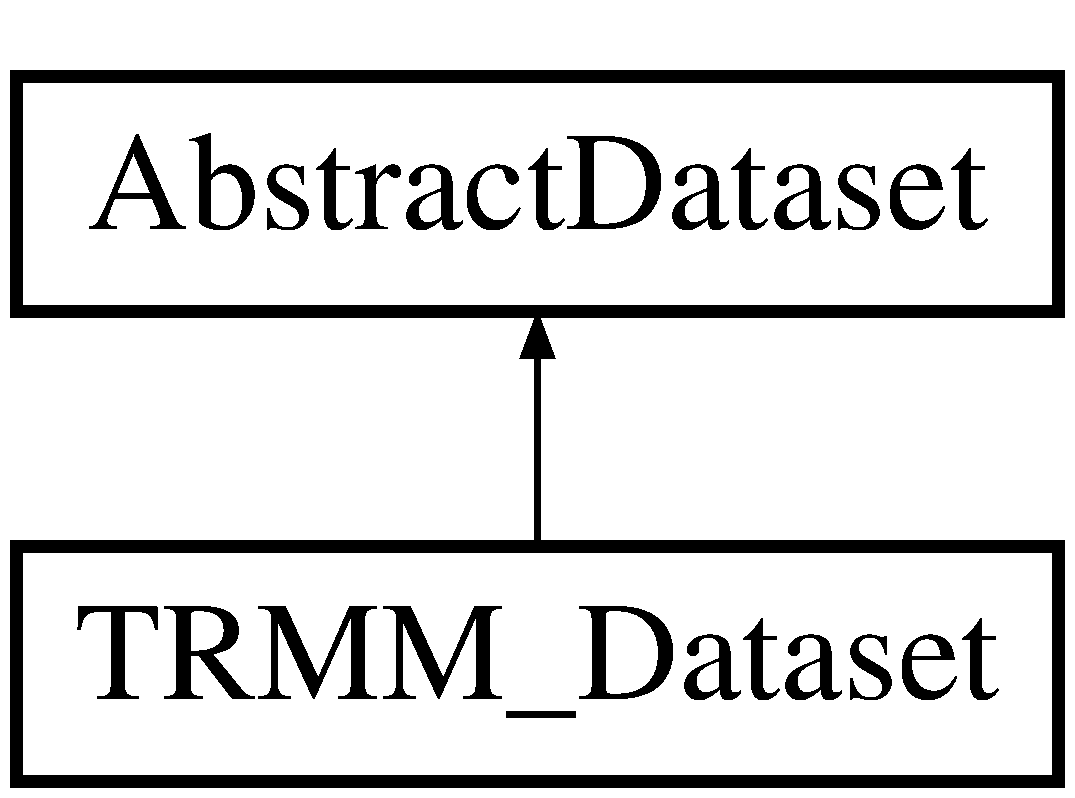
\includegraphics[height=2.000000cm]{classTRMM__Dataset}
\end{center}
\end{figure}
\subsection*{Public Member Functions}
\begin{DoxyCompactItemize}
\item 
virtual \hyperlink{classTRMM__Dataset_a0f192409c4b2fe59ccf4d3ff949112ea}{$\sim$TRMM\_\-Dataset} ()
\begin{DoxyCompactList}\small\item\em Destroy an open \hyperlink{classTRMM__Dataset}{TRMM\_\-Dataset} object. \end{DoxyCompactList}\item 
virtual CPLErr \hyperlink{classTRMM__Dataset_aa08fe6a08a66ab7a115058a302e450a2}{SetMetaDataList} (GDALDataset $\ast$)
\begin{DoxyCompactList}\small\item\em Set the metadata list for this coverage. \end{DoxyCompactList}\item 
virtual CPLErr \hyperlink{classTRMM__Dataset_ac51d16647f04092ee01945f6e627550f}{SetNativeCRS} ()
\begin{DoxyCompactList}\small\item\em Set the Native CRS for a TRMM dataset. \end{DoxyCompactList}\item 
virtual CPLErr \hyperlink{classTRMM__Dataset_afa3309a64ccca14e96628800c69639f8}{SetGeoTransform} ()
\begin{DoxyCompactList}\small\item\em Set the affine GeoTransform matrix for a TRMM coverage. \end{DoxyCompactList}\item 
virtual CPLErr \hyperlink{classTRMM__Dataset_a4c7ca79e2b924ecc42977de339168c14}{SetGDALDataset} (const int isSimple=0)
\begin{DoxyCompactList}\small\item\em Set the GDALDataset object to TRMM dataset. \end{DoxyCompactList}\item 
virtual CPLErr \hyperlink{classTRMM__Dataset_ad1bbde527ce349adee3eacd99d40d2a5}{InitialDataset} (const int isSimple=0)
\begin{DoxyCompactList}\small\item\em Initialize the TRMM dataset . \end{DoxyCompactList}\item 
\hyperlink{classTRMM__Dataset_abcf4bc48213b91a104597302e7e4917b}{TRMM\_\-Dataset} (const string \&id, vector$<$ int $>$ \&rBandList)
\begin{DoxyCompactList}\small\item\em Create an \hyperlink{classTRMM__Dataset}{TRMM\_\-Dataset} object. \end{DoxyCompactList}\end{DoxyCompactItemize}
\subsection*{Public Attributes}
\begin{DoxyCompactItemize}
\item 
\hypertarget{classTRMM__Dataset_a326399d39e963d99900ae8197d9ff841}{
int {\bfseries m\_\-bDaily}}
\label{classTRMM__Dataset_a326399d39e963d99900ae8197d9ff841}

\end{DoxyCompactItemize}


\subsection{Detailed Description}
\hyperlink{classTRMM__Dataset}{TRMM\_\-Dataset} is a subclass of \hyperlink{classAbstractDataset}{AbstractDataset}, used to process TRMM coverage. 

The Tropical Rainfall Measuring Mission (TRMM) is a joint space mission between NASA and the Japan Aerospace Exploration Agency (JAXA) designed to monitor and study tropical rainfall. The term refers to both the mission itself and the satellite that the mission uses to collect data. TRMM is part of NASA's Mission to Planet Earth, a long-\/term, coordinated research effort to study the Earth as a global system. The satellite was launched on November 27, 1997 from the Tanegashima Space Center in Tanegashima, Japan.

\hyperlink{classTRMM__Dataset}{TRMM\_\-Dataset} is a subclass of \hyperlink{classAbstractDataset}{AbstractDataset}, which is used to process TRMM products. 

\subsection{Constructor \& Destructor Documentation}
\hypertarget{classTRMM__Dataset_a0f192409c4b2fe59ccf4d3ff949112ea}{
\index{TRMM\_\-Dataset@{TRMM\_\-Dataset}!$\sim$TRMM\_\-Dataset@{$\sim$TRMM\_\-Dataset}}
\index{$\sim$TRMM\_\-Dataset@{$\sim$TRMM\_\-Dataset}!TRMM_Dataset@{TRMM\_\-Dataset}}
\subsubsection[{$\sim$TRMM\_\-Dataset}]{\setlength{\rightskip}{0pt plus 5cm}TRMM\_\-Dataset::$\sim$TRMM\_\-Dataset (
\begin{DoxyParamCaption}
{}
\end{DoxyParamCaption}
)\hspace{0.3cm}{\ttfamily  \mbox{[}virtual\mbox{]}}}}
\label{classTRMM__Dataset_a0f192409c4b2fe59ccf4d3ff949112ea}


Destroy an open \hyperlink{classTRMM__Dataset}{TRMM\_\-Dataset} object. 

This is the accepted method of closing a \hyperlink{classTRMM__Dataset}{TRMM\_\-Dataset} dataset and deallocating all resources associated with it. \hypertarget{classTRMM__Dataset_abcf4bc48213b91a104597302e7e4917b}{
\index{TRMM\_\-Dataset@{TRMM\_\-Dataset}!TRMM\_\-Dataset@{TRMM\_\-Dataset}}
\index{TRMM\_\-Dataset@{TRMM\_\-Dataset}!TRMM_Dataset@{TRMM\_\-Dataset}}
\subsubsection[{TRMM\_\-Dataset}]{\setlength{\rightskip}{0pt plus 5cm}TRMM\_\-Dataset::TRMM\_\-Dataset (
\begin{DoxyParamCaption}
\item[{const string \&}]{id, }
\item[{vector$<$ int $>$ \&}]{rBandList}
\end{DoxyParamCaption}
)}}
\label{classTRMM__Dataset_abcf4bc48213b91a104597302e7e4917b}


Create an \hyperlink{classTRMM__Dataset}{TRMM\_\-Dataset} object. 

This is the accepted method of creating a \hyperlink{classTRMM__Dataset}{TRMM\_\-Dataset} object and allocating all resources associated with it.


\begin{DoxyParams}{Parameters}
{\em id} & The coverage identifier.\\
\hline
{\em rBandList} & The field list selected for this coverage. For TRMM daily data, the user could specify multiple days range in request. Each day is seemed as one field.\\
\hline
\end{DoxyParams}
\begin{DoxyReturn}{Returns}
A \hyperlink{classTRMM__Dataset}{TRMM\_\-Dataset} object. 
\end{DoxyReturn}


\subsection{Member Function Documentation}
\hypertarget{classTRMM__Dataset_ad1bbde527ce349adee3eacd99d40d2a5}{
\index{TRMM\_\-Dataset@{TRMM\_\-Dataset}!InitialDataset@{InitialDataset}}
\index{InitialDataset@{InitialDataset}!TRMM_Dataset@{TRMM\_\-Dataset}}
\subsubsection[{InitialDataset}]{\setlength{\rightskip}{0pt plus 5cm}CPLErr TRMM\_\-Dataset::InitialDataset (
\begin{DoxyParamCaption}
\item[{const int}]{isSimple = {\ttfamily 0}}
\end{DoxyParamCaption}
)\hspace{0.3cm}{\ttfamily  \mbox{[}virtual\mbox{]}}}}
\label{classTRMM__Dataset_ad1bbde527ce349adee3eacd99d40d2a5}


Initialize the TRMM dataset . 

This method is the implementation for initializing a TRMM dataset. Within this method, \hyperlink{classTRMM__Dataset_ac51d16647f04092ee01945f6e627550f}{SetNativeCRS()}, \hyperlink{classTRMM__Dataset_afa3309a64ccca14e96628800c69639f8}{SetGeoTransform()} and \hyperlink{classTRMM__Dataset_a4c7ca79e2b924ecc42977de339168c14}{SetGDALDataset()} will be called to initialize an TRMM dataset.


\begin{DoxyParams}{Parameters}
{\em isSimple} & the WCS request type. When user executing a DescribeCoverage request, isSimple is set to 1, and for GetCoverage, is set to 0.\\
\hline
\end{DoxyParams}
\begin{DoxyReturn}{Returns}
CE\_\-None on success or CE\_\-Failure on failure. 
\end{DoxyReturn}


Reimplemented from \hyperlink{classAbstractDataset_a45924895c6bf26c7f75d503b8f6e388a}{AbstractDataset}.

\hypertarget{classTRMM__Dataset_a4c7ca79e2b924ecc42977de339168c14}{
\index{TRMM\_\-Dataset@{TRMM\_\-Dataset}!SetGDALDataset@{SetGDALDataset}}
\index{SetGDALDataset@{SetGDALDataset}!TRMM_Dataset@{TRMM\_\-Dataset}}
\subsubsection[{SetGDALDataset}]{\setlength{\rightskip}{0pt plus 5cm}CPLErr TRMM\_\-Dataset::SetGDALDataset (
\begin{DoxyParamCaption}
\item[{const int}]{isSimple = {\ttfamily 0}}
\end{DoxyParamCaption}
)\hspace{0.3cm}{\ttfamily  \mbox{[}virtual\mbox{]}}}}
\label{classTRMM__Dataset_a4c7ca79e2b924ecc42977de339168c14}


Set the GDALDataset object to TRMM dataset. 

This method is used to set the TRMM dataset based on GDAL class VRTDataset.


\begin{DoxyParams}{Parameters}
{\em isSimple} & the WCS request type. When user executing a DescribeCoverage request, isSimple is set to 1, and for GetCoverage, is set to 0.\\
\hline
\end{DoxyParams}
\begin{DoxyReturn}{Returns}
CE\_\-None on success or CE\_\-Failure on failure. 
\end{DoxyReturn}


Reimplemented from \hyperlink{classAbstractDataset_a93bd80bfa48ad45ea53599f289406287}{AbstractDataset}.

\hypertarget{classTRMM__Dataset_afa3309a64ccca14e96628800c69639f8}{
\index{TRMM\_\-Dataset@{TRMM\_\-Dataset}!SetGeoTransform@{SetGeoTransform}}
\index{SetGeoTransform@{SetGeoTransform}!TRMM_Dataset@{TRMM\_\-Dataset}}
\subsubsection[{SetGeoTransform}]{\setlength{\rightskip}{0pt plus 5cm}CPLErr TRMM\_\-Dataset::SetGeoTransform (
\begin{DoxyParamCaption}
{}
\end{DoxyParamCaption}
)\hspace{0.3cm}{\ttfamily  \mbox{[}virtual\mbox{]}}}}
\label{classTRMM__Dataset_afa3309a64ccca14e96628800c69639f8}


Set the affine GeoTransform matrix for a TRMM coverage. 

The method will set a GeoTransform matrix for a TRMM coverage by the pre-\/knowledge of its extent and size.

The CRS for the bounding box is EPSG:4326.

\begin{DoxyReturn}{Returns}
CE\_\-None on success or CE\_\-Failure on failure. 
\end{DoxyReturn}


Reimplemented from \hyperlink{classAbstractDataset_a1d79fc347de75acd57b18c80b9614369}{AbstractDataset}.

\hypertarget{classTRMM__Dataset_aa08fe6a08a66ab7a115058a302e450a2}{
\index{TRMM\_\-Dataset@{TRMM\_\-Dataset}!SetMetaDataList@{SetMetaDataList}}
\index{SetMetaDataList@{SetMetaDataList}!TRMM_Dataset@{TRMM\_\-Dataset}}
\subsubsection[{SetMetaDataList}]{\setlength{\rightskip}{0pt plus 5cm}CPLErr TRMM\_\-Dataset::SetMetaDataList (
\begin{DoxyParamCaption}
\item[{GDALDataset $\ast$}]{hSrcDS}
\end{DoxyParamCaption}
)\hspace{0.3cm}{\ttfamily  \mbox{[}virtual\mbox{]}}}}
\label{classTRMM__Dataset_aa08fe6a08a66ab7a115058a302e450a2}


Set the metadata list for this coverage. 

The method will set the metadata list for the coverage based on its corresponding GDALDataset object.


\begin{DoxyParams}{Parameters}
{\em hSrc} & the GDALDataset object corresponding to coverage.\\
\hline
\end{DoxyParams}
\begin{DoxyReturn}{Returns}
CE\_\-None on success or CE\_\-Failure on failure. 
\end{DoxyReturn}


Reimplemented from \hyperlink{classAbstractDataset_af3f0b55b14f660b79751bf88489a2c10}{AbstractDataset}.

\hypertarget{classTRMM__Dataset_ac51d16647f04092ee01945f6e627550f}{
\index{TRMM\_\-Dataset@{TRMM\_\-Dataset}!SetNativeCRS@{SetNativeCRS}}
\index{SetNativeCRS@{SetNativeCRS}!TRMM_Dataset@{TRMM\_\-Dataset}}
\subsubsection[{SetNativeCRS}]{\setlength{\rightskip}{0pt plus 5cm}CPLErr TRMM\_\-Dataset::SetNativeCRS (
\begin{DoxyParamCaption}
{}
\end{DoxyParamCaption}
)\hspace{0.3cm}{\ttfamily  \mbox{[}virtual\mbox{]}}}}
\label{classTRMM__Dataset_ac51d16647f04092ee01945f6e627550f}


Set the Native CRS for a TRMM dataset. 

The method will set the CRS for a TRMM dataset as an native CRS.

The native CRS for TRMM is assigned to EPSG:4326.

\begin{DoxyReturn}{Returns}
CE\_\-None on success or CE\_\-Failure on failure. 
\end{DoxyReturn}


Reimplemented from \hyperlink{classAbstractDataset_acfac922d16e5edf51066169bd6ff28ec}{AbstractDataset}.



The documentation for this class was generated from the following files:\begin{DoxyCompactItemize}
\item 
TRMM\_\-Dataset.h\item 
TRMM\_\-Dataset.cpp\end{DoxyCompactItemize}

\hypertarget{classWCS__Configure}{
\section{WCS\_\-Configure Class Reference}
\label{classWCS__Configure}\index{WCS\_\-Configure@{WCS\_\-Configure}}
}


Configuration class provides fetch methods to get information from WCS configuration file.  




{\ttfamily \#include $<$WCS\_\-Configure.h$>$}

\subsection*{Public Member Functions}
\begin{DoxyCompactItemize}
\item 
\hyperlink{classWCS__Configure_a8f0f3520d76723409b2290ce3d5ec3de}{WCS\_\-Configure} ()
\item 
\hyperlink{classWCS__Configure_a69a5f47a39b58a80f3ba4baaf32c9693}{WCS\_\-Configure} (const string \&conf)
\begin{DoxyCompactList}\small\item\em Constructor of an \hyperlink{classWCS__Configure}{WCS\_\-Configure} object. \end{DoxyCompactList}\item 
string \hyperlink{classWCS__Configure_a17e6c9417cf036ab459e1cd36aadcdaa}{Get\_\-CAPABILITIES\_\-HEAD\_\-FILE\_\-PATH} ()
\begin{DoxyCompactList}\small\item\em Fetch the XML head element of the capabilities document. \end{DoxyCompactList}\item 
string \hyperlink{classWCS__Configure_aa24220528f8fc68dd379db5b95943dd2}{Get\_\-CAPABILITIES\_\-SEVICEIDENTIFICATION\_\-FILE\_\-PATH} ()
\begin{DoxyCompactList}\small\item\em Fetch the ServiceIdentification part of the capabilities document. \end{DoxyCompactList}\item 
string \hyperlink{classWCS__Configure_a4d6eca21bef095f73a75f8c1d74c32eb}{Get\_\-CAPABILITIES\_\-SEVICEPROVIDER\_\-FILE\_\-PATH} ()
\begin{DoxyCompactList}\small\item\em Fetch the ServiceProvider part of the capabilities document. \end{DoxyCompactList}\item 
string \hyperlink{classWCS__Configure_ae565e9adcf4513f0de954e422017cadf}{Get\_\-CAPABILITIES\_\-OPERATIONSMETADA\_\-FILE\_\-PATH} ()
\begin{DoxyCompactList}\small\item\em Fetch the OperationsMetadata part of the capabilities document. \end{DoxyCompactList}\item 
string \hyperlink{classWCS__Configure_aeec65d726fddb454ec9c943ef46602ca}{Get\_\-CAPABILITIES\_\-CONTENTS\_\-FILE\_\-PATH} ()
\begin{DoxyCompactList}\small\item\em Fetch the Contents part of the capabilities document. \end{DoxyCompactList}\item 
string \hyperlink{classWCS__Configure_afdecaaadfc30c79f6766b606fd05b402}{Get\_\-SERVICE\_\-ACCESS\_\-URL} ()
\begin{DoxyCompactList}\small\item\em Fetch the access URL of this WCS. \end{DoxyCompactList}\item 
string \hyperlink{classWCS__Configure_abd5989379bf561c53c7c14d37a8f99e9}{Get\_\-WCS\_\-SERVICE\_\-DATA\_\-DIRECTORY} ()
\begin{DoxyCompactList}\small\item\em Fetch the directory of the data-\/to-\/be-\/served. \end{DoxyCompactList}\item 
string \hyperlink{classWCS__Configure_a82ce7ca820eed3e38a66a1befb885e4b}{Get\_\-DATASET\_\-CONFIGRATION\_\-FILE\_\-PATH} ()
\begin{DoxyCompactList}\small\item\em Fetch the configuration XML file path of dataset coverage. \end{DoxyCompactList}\item 
string \hyperlink{classWCS__Configure_ae0fc8963b3530a687c0b6fca39e28519}{Get\_\-STITCHED\_\-MOSAIC\_\-CONFIGRATION\_\-FILE\_\-PATH} ()
\begin{DoxyCompactList}\small\item\em Fetch the configuration XML file path of stitched mosaic coverage. \end{DoxyCompactList}\item 
string \hyperlink{classWCS__Configure_a6aeb058758db3aab635af53dbcf5e7b2}{Get\_\-DATASET\_\-SERIES\_\-CONFIGRATION\_\-FILE\_\-PATH} ()
\begin{DoxyCompactList}\small\item\em Fetch the configuration XML file path of datasetSeries coverage. \end{DoxyCompactList}\item 
string \hyperlink{classWCS__Configure_af82cfb1889f6ba7ce9a44dc644f2badc}{Get\_\-TRANSACTION\_\-DATA\_\-DIRECTORY} ()
\begin{DoxyCompactList}\small\item\em Fetch the directory for placing the data will be transacted. \end{DoxyCompactList}\item 
string \hyperlink{classWCS__Configure_af4ae701e12b38013a75938e44b9cac54}{Get\_\-TEMPORARY\_\-OUTPUT\_\-DIRECTORY} ()
\begin{DoxyCompactList}\small\item\em Fetch the directory for placing temporary and output files. \end{DoxyCompactList}\item 
string \hyperlink{classWCS__Configure_a102b44721354ea7267a39d0ad06acee7}{Get\_\-OUTPUT\_\-PREFIX\_\-URL} ()
\begin{DoxyCompactList}\small\item\em Fetch the URL prefix corresponding to the temporary directory. \end{DoxyCompactList}\item 
string \hyperlink{classWCS__Configure_a484861bea7a237b7bc8a69aaee45fe9d}{Get\_\-CAPABILITIES\_\-FILE\_\-PATH} ()
\begin{DoxyCompactList}\small\item\em Fetch the path of the capabilities file path. \end{DoxyCompactList}\item 
string \hyperlink{classWCS__Configure_a9620adfd4bf1f21d35a1be4e2e2842d7}{Get\_\-WCS\_\-LOGFILE\_\-PATH} ()
\begin{DoxyCompactList}\small\item\em Fetch the path of the WCS log file path. \end{DoxyCompactList}\item 
string \hyperlink{classWCS__Configure_a8f7718a4c34d9c008ed908b53b87d85b}{Get\_\-GDAL\_\-WARP\_\-PATH} ()
\begin{DoxyCompactList}\small\item\em Fetch the path of gdalwap command line. \end{DoxyCompactList}\item 
string \hyperlink{classWCS__Configure_a31326fa9c015dc8c5fb79072b1af9ddd}{Get\_\-ISO\_\-19115\_\-METADATA\_\-TEMPLATE\_\-PATH} ()
\begin{DoxyCompactList}\small\item\em Fetch the path of the ISO 19115 template file. \end{DoxyCompactList}\item 
string \hyperlink{classWCS__Configure_a9d9c703b2c3fdde176e5b89a52786548}{GetConfigureFileName} ()
\begin{DoxyCompactList}\small\item\em Fetch the full path of the configuration file. \end{DoxyCompactList}\end{DoxyCompactItemize}


\subsection{Detailed Description}
Configuration class provides fetch methods to get information from WCS configuration file. 

A configuration file contains WCS-\/related parameters, which is placed under the same directory with WCS executable. The configuration file also has the same name with WCS executable but plus an suffix \char`\"{}conf\char`\"{}.

This configuration file is required for WCS service. 

\subsection{Constructor \& Destructor Documentation}
\hypertarget{classWCS__Configure_a8f0f3520d76723409b2290ce3d5ec3de}{
\index{WCS\_\-Configure@{WCS\_\-Configure}!WCS\_\-Configure@{WCS\_\-Configure}}
\index{WCS\_\-Configure@{WCS\_\-Configure}!WCS_Configure@{WCS\_\-Configure}}
\subsubsection[{WCS\_\-Configure}]{\setlength{\rightskip}{0pt plus 5cm}WCS\_\-Configure::WCS\_\-Configure (
\begin{DoxyParamCaption}
{}
\end{DoxyParamCaption}
)}}
\label{classWCS__Configure_a8f0f3520d76723409b2290ce3d5ec3de}
Constructor of an \hyperlink{classWCS__Configure}{WCS\_\-Configure} object. \hypertarget{classWCS__Configure_a69a5f47a39b58a80f3ba4baaf32c9693}{
\index{WCS\_\-Configure@{WCS\_\-Configure}!WCS\_\-Configure@{WCS\_\-Configure}}
\index{WCS\_\-Configure@{WCS\_\-Configure}!WCS_Configure@{WCS\_\-Configure}}
\subsubsection[{WCS\_\-Configure}]{\setlength{\rightskip}{0pt plus 5cm}WCS\_\-Configure::WCS\_\-Configure (
\begin{DoxyParamCaption}
\item[{const string \&}]{conf}
\end{DoxyParamCaption}
)}}
\label{classWCS__Configure_a69a5f47a39b58a80f3ba4baaf32c9693}


Constructor of an \hyperlink{classWCS__Configure}{WCS\_\-Configure} object. 

This is the accepted method of creating an configuration object and based this object to read the configuration information.


\begin{DoxyParams}{Parameters}
{\em conf} & String of the full path of the configuration file. \\
\hline
\end{DoxyParams}


\subsection{Member Function Documentation}
\hypertarget{classWCS__Configure_aeec65d726fddb454ec9c943ef46602ca}{
\index{WCS\_\-Configure@{WCS\_\-Configure}!Get\_\-CAPABILITIES\_\-CONTENTS\_\-FILE\_\-PATH@{Get\_\-CAPABILITIES\_\-CONTENTS\_\-FILE\_\-PATH}}
\index{Get\_\-CAPABILITIES\_\-CONTENTS\_\-FILE\_\-PATH@{Get\_\-CAPABILITIES\_\-CONTENTS\_\-FILE\_\-PATH}!WCS_Configure@{WCS\_\-Configure}}
\subsubsection[{Get\_\-CAPABILITIES\_\-CONTENTS\_\-FILE\_\-PATH}]{\setlength{\rightskip}{0pt plus 5cm}string WCS\_\-Configure::Get\_\-CAPABILITIES\_\-CONTENTS\_\-FILE\_\-PATH (
\begin{DoxyParamCaption}
{}
\end{DoxyParamCaption}
)}}
\label{classWCS__Configure_aeec65d726fddb454ec9c943ef46602ca}


Fetch the Contents part of the capabilities document. 

This method will return the Contents part of the capabilities document.

\begin{DoxyReturn}{Returns}
String of the Contents part of the capabilities document. 
\end{DoxyReturn}
\hypertarget{classWCS__Configure_a484861bea7a237b7bc8a69aaee45fe9d}{
\index{WCS\_\-Configure@{WCS\_\-Configure}!Get\_\-CAPABILITIES\_\-FILE\_\-PATH@{Get\_\-CAPABILITIES\_\-FILE\_\-PATH}}
\index{Get\_\-CAPABILITIES\_\-FILE\_\-PATH@{Get\_\-CAPABILITIES\_\-FILE\_\-PATH}!WCS_Configure@{WCS\_\-Configure}}
\subsubsection[{Get\_\-CAPABILITIES\_\-FILE\_\-PATH}]{\setlength{\rightskip}{0pt plus 5cm}string WCS\_\-Configure::Get\_\-CAPABILITIES\_\-FILE\_\-PATH (
\begin{DoxyParamCaption}
{}
\end{DoxyParamCaption}
)}}
\label{classWCS__Configure_a484861bea7a237b7bc8a69aaee45fe9d}


Fetch the path of the capabilities file path. 

This method will return the path of the capabilities file path. If this value is specified, WCS will import the file specified and display the XML contents to user.

\begin{DoxyReturn}{Returns}
String of the path of the capabilities file path. 
\end{DoxyReturn}
\hypertarget{classWCS__Configure_a17e6c9417cf036ab459e1cd36aadcdaa}{
\index{WCS\_\-Configure@{WCS\_\-Configure}!Get\_\-CAPABILITIES\_\-HEAD\_\-FILE\_\-PATH@{Get\_\-CAPABILITIES\_\-HEAD\_\-FILE\_\-PATH}}
\index{Get\_\-CAPABILITIES\_\-HEAD\_\-FILE\_\-PATH@{Get\_\-CAPABILITIES\_\-HEAD\_\-FILE\_\-PATH}!WCS_Configure@{WCS\_\-Configure}}
\subsubsection[{Get\_\-CAPABILITIES\_\-HEAD\_\-FILE\_\-PATH}]{\setlength{\rightskip}{0pt plus 5cm}string WCS\_\-Configure::Get\_\-CAPABILITIES\_\-HEAD\_\-FILE\_\-PATH (
\begin{DoxyParamCaption}
{}
\end{DoxyParamCaption}
)}}
\label{classWCS__Configure_a17e6c9417cf036ab459e1cd36aadcdaa}


Fetch the XML head element of the capabilities document. 

This method will return the XML head element of the capabilities document.

\begin{DoxyReturn}{Returns}
String of the head element of the capabilities document. 
\end{DoxyReturn}
\hypertarget{classWCS__Configure_ae565e9adcf4513f0de954e422017cadf}{
\index{WCS\_\-Configure@{WCS\_\-Configure}!Get\_\-CAPABILITIES\_\-OPERATIONSMETADA\_\-FILE\_\-PATH@{Get\_\-CAPABILITIES\_\-OPERATIONSMETADA\_\-FILE\_\-PATH}}
\index{Get\_\-CAPABILITIES\_\-OPERATIONSMETADA\_\-FILE\_\-PATH@{Get\_\-CAPABILITIES\_\-OPERATIONSMETADA\_\-FILE\_\-PATH}!WCS_Configure@{WCS\_\-Configure}}
\subsubsection[{Get\_\-CAPABILITIES\_\-OPERATIONSMETADA\_\-FILE\_\-PATH}]{\setlength{\rightskip}{0pt plus 5cm}string WCS\_\-Configure::Get\_\-CAPABILITIES\_\-OPERATIONSMETADA\_\-FILE\_\-PATH (
\begin{DoxyParamCaption}
{}
\end{DoxyParamCaption}
)}}
\label{classWCS__Configure_ae565e9adcf4513f0de954e422017cadf}


Fetch the OperationsMetadata part of the capabilities document. 

This method will return the OperationsMetadata part of the capabilities document.

\begin{DoxyReturn}{Returns}
String of the OperationsMetadata part of the capabilities document. 
\end{DoxyReturn}
\hypertarget{classWCS__Configure_aa24220528f8fc68dd379db5b95943dd2}{
\index{WCS\_\-Configure@{WCS\_\-Configure}!Get\_\-CAPABILITIES\_\-SEVICEIDENTIFICATION\_\-FILE\_\-PATH@{Get\_\-CAPABILITIES\_\-SEVICEIDENTIFICATION\_\-FILE\_\-PATH}}
\index{Get\_\-CAPABILITIES\_\-SEVICEIDENTIFICATION\_\-FILE\_\-PATH@{Get\_\-CAPABILITIES\_\-SEVICEIDENTIFICATION\_\-FILE\_\-PATH}!WCS_Configure@{WCS\_\-Configure}}
\subsubsection[{Get\_\-CAPABILITIES\_\-SEVICEIDENTIFICATION\_\-FILE\_\-PATH}]{\setlength{\rightskip}{0pt plus 5cm}string WCS\_\-Configure::Get\_\-CAPABILITIES\_\-SEVICEIDENTIFICATION\_\-FILE\_\-PATH (
\begin{DoxyParamCaption}
{}
\end{DoxyParamCaption}
)}}
\label{classWCS__Configure_aa24220528f8fc68dd379db5b95943dd2}


Fetch the ServiceIdentification part of the capabilities document. 

This method will return the ServiceIdentification part of the capabilities document.

\begin{DoxyReturn}{Returns}
String of the ServiceIdentification part of the capabilities document. 
\end{DoxyReturn}
\hypertarget{classWCS__Configure_a4d6eca21bef095f73a75f8c1d74c32eb}{
\index{WCS\_\-Configure@{WCS\_\-Configure}!Get\_\-CAPABILITIES\_\-SEVICEPROVIDER\_\-FILE\_\-PATH@{Get\_\-CAPABILITIES\_\-SEVICEPROVIDER\_\-FILE\_\-PATH}}
\index{Get\_\-CAPABILITIES\_\-SEVICEPROVIDER\_\-FILE\_\-PATH@{Get\_\-CAPABILITIES\_\-SEVICEPROVIDER\_\-FILE\_\-PATH}!WCS_Configure@{WCS\_\-Configure}}
\subsubsection[{Get\_\-CAPABILITIES\_\-SEVICEPROVIDER\_\-FILE\_\-PATH}]{\setlength{\rightskip}{0pt plus 5cm}string WCS\_\-Configure::Get\_\-CAPABILITIES\_\-SEVICEPROVIDER\_\-FILE\_\-PATH (
\begin{DoxyParamCaption}
{}
\end{DoxyParamCaption}
)}}
\label{classWCS__Configure_a4d6eca21bef095f73a75f8c1d74c32eb}


Fetch the ServiceProvider part of the capabilities document. 

This method will return the ServiceProvider part of the capabilities document.

\begin{DoxyReturn}{Returns}
String of the ServiceProvider part of the capabilities document. 
\end{DoxyReturn}
\hypertarget{classWCS__Configure_a82ce7ca820eed3e38a66a1befb885e4b}{
\index{WCS\_\-Configure@{WCS\_\-Configure}!Get\_\-DATASET\_\-CONFIGRATION\_\-FILE\_\-PATH@{Get\_\-DATASET\_\-CONFIGRATION\_\-FILE\_\-PATH}}
\index{Get\_\-DATASET\_\-CONFIGRATION\_\-FILE\_\-PATH@{Get\_\-DATASET\_\-CONFIGRATION\_\-FILE\_\-PATH}!WCS_Configure@{WCS\_\-Configure}}
\subsubsection[{Get\_\-DATASET\_\-CONFIGRATION\_\-FILE\_\-PATH}]{\setlength{\rightskip}{0pt plus 5cm}string WCS\_\-Configure::Get\_\-DATASET\_\-CONFIGRATION\_\-FILE\_\-PATH (
\begin{DoxyParamCaption}
{}
\end{DoxyParamCaption}
)}}
\label{classWCS__Configure_a82ce7ca820eed3e38a66a1befb885e4b}


Fetch the configuration XML file path of dataset coverage. 

To improve the performance of WCS and make it easy to add the support to new datasets, some specified information of each dataset/granule will be extracted and build a XML file based on those information, such as coverage identifier in GDAL, bounding box, temporal range, coverage name to-\/be-\/displayed to user.

On dataset's configuration file could include many dataset, and also the values of 'DATASET\_\-CONFIGRATION\_\-FILE\_\-PATH' could be specified by multiple dataset's configuration files, separated by ',' or ';'.

Sample: 
\begin{DoxyCode}
 <Datasets>
   <Dataset>
     <name>MOD05_L2.A2008205.0255.005.2008206170326.hdf:Water_Vapor_Infrared</nam
      e>
           <path>/home/yshao/data/</path>
           <coverageID>HDF4_EOS:EOS_SWATH:"/home/yshao/data/MOD05_L2.A2008205.025
      5.005.2008206170326.hdf":mod05:Water_Vapor_Infrared</coverageID>
           <west>-93.8909</west>
           <east>-59.1097</east>
           <south>32.2516</south>
           <north>53.7898</north>
           <beginTime>2008-07-23T02:55:00Z</beginTime>
           <endTime>2008-07-23T03:00:00Z</endTime>
     </Dataset>
   <Dataset>
     ...
   </Dataset>
 </Datasets>
\end{DoxyCode}


\begin{DoxyReturn}{Returns}
String of the paths of the dataset's configuration file. 
\end{DoxyReturn}
\hypertarget{classWCS__Configure_a6aeb058758db3aab635af53dbcf5e7b2}{
\index{WCS\_\-Configure@{WCS\_\-Configure}!Get\_\-DATASET\_\-SERIES\_\-CONFIGRATION\_\-FILE\_\-PATH@{Get\_\-DATASET\_\-SERIES\_\-CONFIGRATION\_\-FILE\_\-PATH}}
\index{Get\_\-DATASET\_\-SERIES\_\-CONFIGRATION\_\-FILE\_\-PATH@{Get\_\-DATASET\_\-SERIES\_\-CONFIGRATION\_\-FILE\_\-PATH}!WCS_Configure@{WCS\_\-Configure}}
\subsubsection[{Get\_\-DATASET\_\-SERIES\_\-CONFIGRATION\_\-FILE\_\-PATH}]{\setlength{\rightskip}{0pt plus 5cm}string WCS\_\-Configure::Get\_\-DATASET\_\-SERIES\_\-CONFIGRATION\_\-FILE\_\-PATH (
\begin{DoxyParamCaption}
{}
\end{DoxyParamCaption}
)}}
\label{classWCS__Configure_a6aeb058758db3aab635af53dbcf5e7b2}


Fetch the configuration XML file path of datasetSeries coverage. 

To improve the performance of WCS and make it easy to add the support to new datasetSeries coverage, some specified information of each dataset/granule within the dataset series will be extracted and build a XML file based on those information.

Sample: 
\begin{DoxyCode}
 <WCSEODatasetSeries>
 <DatasetSeries>
 <DatasetSeriesId>MODIS_Vegetation_Indices_NDVI_16-Day_L3_Global_0.05Deg_Year_201
      0</DatasetSeriesId>
 <CollectionName>MOD13C1</CollectionName>
 <CoverageName>CMG 0.05 Deg 16 days NDVI</CoverageName>
 <Datasets>
 <Dataset>
 <name>MOD13C1.A2010289.005.2010310073051.hdf</name>
 <path>/home/yshao/data/MOD13C1.A2010289.005.2010310073051.hdf</path>
 <coverageID>HDF4_EOS:EOS_GRID:"/home/yshao/data/MOD13C1.A2010289.005.20103100730
      51.hdf":MODIS_Grid_16Day_VI_CMG:CMG 0.05 Deg 16 days NDVI</coverageID>
 <west>-180</west>
 <east>180</east>
 <south>-90</south>
 <north>90</north>
 <beginTime>2010-07-28T00:00:00Z</beginTime>
 <endTime>2010-08-12T23:59:59Z</endTime>
 </Dataset>
 <Dataset>
 ...
 </Dataset>
 </Datasets>
 </DatasetSeries>
 <DatasetSeries>
 ...
 </DatasetSeries>
 </WCSEODatasetSeries>
\end{DoxyCode}


\begin{DoxyReturn}{Returns}
String of the paths of the dataset series' configuration file. 
\end{DoxyReturn}
\hypertarget{classWCS__Configure_a8f7718a4c34d9c008ed908b53b87d85b}{
\index{WCS\_\-Configure@{WCS\_\-Configure}!Get\_\-GDAL\_\-WARP\_\-PATH@{Get\_\-GDAL\_\-WARP\_\-PATH}}
\index{Get\_\-GDAL\_\-WARP\_\-PATH@{Get\_\-GDAL\_\-WARP\_\-PATH}!WCS_Configure@{WCS\_\-Configure}}
\subsubsection[{Get\_\-GDAL\_\-WARP\_\-PATH}]{\setlength{\rightskip}{0pt plus 5cm}string WCS\_\-Configure::Get\_\-GDAL\_\-WARP\_\-PATH (
\begin{DoxyParamCaption}
{}
\end{DoxyParamCaption}
)}}
\label{classWCS__Configure_a8f7718a4c34d9c008ed908b53b87d85b}


Fetch the path of gdalwap command line. 

This method will return the path of gdalwap command line

\begin{DoxyReturn}{Returns}
String of the path of gdalwap command line 
\end{DoxyReturn}
\hypertarget{classWCS__Configure_a31326fa9c015dc8c5fb79072b1af9ddd}{
\index{WCS\_\-Configure@{WCS\_\-Configure}!Get\_\-ISO\_\-19115\_\-METADATA\_\-TEMPLATE\_\-PATH@{Get\_\-ISO\_\-19115\_\-METADATA\_\-TEMPLATE\_\-PATH}}
\index{Get\_\-ISO\_\-19115\_\-METADATA\_\-TEMPLATE\_\-PATH@{Get\_\-ISO\_\-19115\_\-METADATA\_\-TEMPLATE\_\-PATH}!WCS_Configure@{WCS\_\-Configure}}
\subsubsection[{Get\_\-ISO\_\-19115\_\-METADATA\_\-TEMPLATE\_\-PATH}]{\setlength{\rightskip}{0pt plus 5cm}string WCS\_\-Configure::Get\_\-ISO\_\-19115\_\-METADATA\_\-TEMPLATE\_\-PATH (
\begin{DoxyParamCaption}
{}
\end{DoxyParamCaption}
)}}
\label{classWCS__Configure_a31326fa9c015dc8c5fb79072b1af9ddd}


Fetch the path of the ISO 19115 template file. 

This method will return the path of the ISO 19115 template file.

\begin{DoxyReturn}{Returns}
String of the path of the ISO 19115 template file. 
\end{DoxyReturn}
\hypertarget{classWCS__Configure_a102b44721354ea7267a39d0ad06acee7}{
\index{WCS\_\-Configure@{WCS\_\-Configure}!Get\_\-OUTPUT\_\-PREFIX\_\-URL@{Get\_\-OUTPUT\_\-PREFIX\_\-URL}}
\index{Get\_\-OUTPUT\_\-PREFIX\_\-URL@{Get\_\-OUTPUT\_\-PREFIX\_\-URL}!WCS_Configure@{WCS\_\-Configure}}
\subsubsection[{Get\_\-OUTPUT\_\-PREFIX\_\-URL}]{\setlength{\rightskip}{0pt plus 5cm}string WCS\_\-Configure::Get\_\-OUTPUT\_\-PREFIX\_\-URL (
\begin{DoxyParamCaption}
{}
\end{DoxyParamCaption}
)}}
\label{classWCS__Configure_a102b44721354ea7267a39d0ad06acee7}


Fetch the URL prefix corresponding to the temporary directory. 

This method will return the URL prefix corresponding to the temporary directory.

\begin{DoxyReturn}{Returns}
String of the URL prefix corresponding to the temporary directory. 
\end{DoxyReturn}
\hypertarget{classWCS__Configure_afdecaaadfc30c79f6766b606fd05b402}{
\index{WCS\_\-Configure@{WCS\_\-Configure}!Get\_\-SERVICE\_\-ACCESS\_\-URL@{Get\_\-SERVICE\_\-ACCESS\_\-URL}}
\index{Get\_\-SERVICE\_\-ACCESS\_\-URL@{Get\_\-SERVICE\_\-ACCESS\_\-URL}!WCS_Configure@{WCS\_\-Configure}}
\subsubsection[{Get\_\-SERVICE\_\-ACCESS\_\-URL}]{\setlength{\rightskip}{0pt plus 5cm}string WCS\_\-Configure::Get\_\-SERVICE\_\-ACCESS\_\-URL (
\begin{DoxyParamCaption}
{}
\end{DoxyParamCaption}
)}}
\label{classWCS__Configure_afdecaaadfc30c79f6766b606fd05b402}


Fetch the access URL of this WCS. 

This method will return the access URL of this WCS.

\begin{DoxyReturn}{Returns}
String of the access URL of this WCS. 
\end{DoxyReturn}
\hypertarget{classWCS__Configure_ae0fc8963b3530a687c0b6fca39e28519}{
\index{WCS\_\-Configure@{WCS\_\-Configure}!Get\_\-STITCHED\_\-MOSAIC\_\-CONFIGRATION\_\-FILE\_\-PATH@{Get\_\-STITCHED\_\-MOSAIC\_\-CONFIGRATION\_\-FILE\_\-PATH}}
\index{Get\_\-STITCHED\_\-MOSAIC\_\-CONFIGRATION\_\-FILE\_\-PATH@{Get\_\-STITCHED\_\-MOSAIC\_\-CONFIGRATION\_\-FILE\_\-PATH}!WCS_Configure@{WCS\_\-Configure}}
\subsubsection[{Get\_\-STITCHED\_\-MOSAIC\_\-CONFIGRATION\_\-FILE\_\-PATH}]{\setlength{\rightskip}{0pt plus 5cm}string WCS\_\-Configure::Get\_\-STITCHED\_\-MOSAIC\_\-CONFIGRATION\_\-FILE\_\-PATH (
\begin{DoxyParamCaption}
{}
\end{DoxyParamCaption}
)}}
\label{classWCS__Configure_ae0fc8963b3530a687c0b6fca39e28519}


Fetch the configuration XML file path of stitched mosaic coverage. 

To improve the performance of WCS and make it easy to add the support to new mosaic coverage, some specified information of each dataset/granule within the mosaic coverage will be extracted and build a XML file based on those information.

\begin{Desc}
\item[\hyperlink{todo__todo000001}{Todo}]Currently (as of 07/22) the GMU WCS did not serve the data in the form of mosaic coverage, some demos will be added based on new requirement.\end{Desc}


\begin{DoxyReturn}{Returns}
String of the paths of the mosaic coverage's configuration file. 
\end{DoxyReturn}
\hypertarget{classWCS__Configure_af4ae701e12b38013a75938e44b9cac54}{
\index{WCS\_\-Configure@{WCS\_\-Configure}!Get\_\-TEMPORARY\_\-OUTPUT\_\-DIRECTORY@{Get\_\-TEMPORARY\_\-OUTPUT\_\-DIRECTORY}}
\index{Get\_\-TEMPORARY\_\-OUTPUT\_\-DIRECTORY@{Get\_\-TEMPORARY\_\-OUTPUT\_\-DIRECTORY}!WCS_Configure@{WCS\_\-Configure}}
\subsubsection[{Get\_\-TEMPORARY\_\-OUTPUT\_\-DIRECTORY}]{\setlength{\rightskip}{0pt plus 5cm}string WCS\_\-Configure::Get\_\-TEMPORARY\_\-OUTPUT\_\-DIRECTORY (
\begin{DoxyParamCaption}
{}
\end{DoxyParamCaption}
)}}
\label{classWCS__Configure_af4ae701e12b38013a75938e44b9cac54}


Fetch the directory for placing temporary and output files. 

This method will return the directory for placing temporary and output files.

\begin{DoxyReturn}{Returns}
String of the directory for placing temporary and output files. 
\end{DoxyReturn}
\hypertarget{classWCS__Configure_af82cfb1889f6ba7ce9a44dc644f2badc}{
\index{WCS\_\-Configure@{WCS\_\-Configure}!Get\_\-TRANSACTION\_\-DATA\_\-DIRECTORY@{Get\_\-TRANSACTION\_\-DATA\_\-DIRECTORY}}
\index{Get\_\-TRANSACTION\_\-DATA\_\-DIRECTORY@{Get\_\-TRANSACTION\_\-DATA\_\-DIRECTORY}!WCS_Configure@{WCS\_\-Configure}}
\subsubsection[{Get\_\-TRANSACTION\_\-DATA\_\-DIRECTORY}]{\setlength{\rightskip}{0pt plus 5cm}string WCS\_\-Configure::Get\_\-TRANSACTION\_\-DATA\_\-DIRECTORY (
\begin{DoxyParamCaption}
{}
\end{DoxyParamCaption}
)}}
\label{classWCS__Configure_af82cfb1889f6ba7ce9a44dc644f2badc}


Fetch the directory for placing the data will be transacted. 

This method will return the directory for placing the data will be transacted.

\begin{Desc}
\item[\hyperlink{todo__todo000002}{Todo}]Currently (as of 07/22) the transaction interface of GMU WCS have not been tested.\end{Desc}


\begin{DoxyReturn}{Returns}
String of the directory of the data-\/to-\/be-\/served. 
\end{DoxyReturn}
\hypertarget{classWCS__Configure_a9620adfd4bf1f21d35a1be4e2e2842d7}{
\index{WCS\_\-Configure@{WCS\_\-Configure}!Get\_\-WCS\_\-LOGFILE\_\-PATH@{Get\_\-WCS\_\-LOGFILE\_\-PATH}}
\index{Get\_\-WCS\_\-LOGFILE\_\-PATH@{Get\_\-WCS\_\-LOGFILE\_\-PATH}!WCS_Configure@{WCS\_\-Configure}}
\subsubsection[{Get\_\-WCS\_\-LOGFILE\_\-PATH}]{\setlength{\rightskip}{0pt plus 5cm}string WCS\_\-Configure::Get\_\-WCS\_\-LOGFILE\_\-PATH (
\begin{DoxyParamCaption}
{}
\end{DoxyParamCaption}
)}}
\label{classWCS__Configure_a9620adfd4bf1f21d35a1be4e2e2842d7}


Fetch the path of the WCS log file path. 

This method will return the path of the WCS log file path.

\begin{DoxyReturn}{Returns}
String of the path of the WCS log file path. 
\end{DoxyReturn}
\hypertarget{classWCS__Configure_abd5989379bf561c53c7c14d37a8f99e9}{
\index{WCS\_\-Configure@{WCS\_\-Configure}!Get\_\-WCS\_\-SERVICE\_\-DATA\_\-DIRECTORY@{Get\_\-WCS\_\-SERVICE\_\-DATA\_\-DIRECTORY}}
\index{Get\_\-WCS\_\-SERVICE\_\-DATA\_\-DIRECTORY@{Get\_\-WCS\_\-SERVICE\_\-DATA\_\-DIRECTORY}!WCS_Configure@{WCS\_\-Configure}}
\subsubsection[{Get\_\-WCS\_\-SERVICE\_\-DATA\_\-DIRECTORY}]{\setlength{\rightskip}{0pt plus 5cm}string WCS\_\-Configure::Get\_\-WCS\_\-SERVICE\_\-DATA\_\-DIRECTORY (
\begin{DoxyParamCaption}
{}
\end{DoxyParamCaption}
)}}
\label{classWCS__Configure_abd5989379bf561c53c7c14d37a8f99e9}


Fetch the directory of the data-\/to-\/be-\/served. 

This method will return the directory of the data-\/to-\/be-\/served.

\begin{DoxyReturn}{Returns}
String of the directory of the data-\/to-\/be-\/served. 
\end{DoxyReturn}
\hypertarget{classWCS__Configure_a9d9c703b2c3fdde176e5b89a52786548}{
\index{WCS\_\-Configure@{WCS\_\-Configure}!GetConfigureFileName@{GetConfigureFileName}}
\index{GetConfigureFileName@{GetConfigureFileName}!WCS_Configure@{WCS\_\-Configure}}
\subsubsection[{GetConfigureFileName}]{\setlength{\rightskip}{0pt plus 5cm}string WCS\_\-Configure::GetConfigureFileName (
\begin{DoxyParamCaption}
{}
\end{DoxyParamCaption}
)}}
\label{classWCS__Configure_a9d9c703b2c3fdde176e5b89a52786548}


Fetch the full path of the configuration file. 

This method will return the full path of the configuration file.

\begin{DoxyReturn}{Returns}
String of the full path of the configuration file. 
\end{DoxyReturn}


The documentation for this class was generated from the following files:\begin{DoxyCompactItemize}
\item 
WCS\_\-Configure.h\item 
WCS\_\-Configure.cpp\end{DoxyCompactItemize}

\hypertarget{classWCS__DescribeCoverage}{
\section{WCS\_\-DescribeCoverage Class Reference}
\label{classWCS__DescribeCoverage}\index{WCS\_\-DescribeCoverage@{WCS\_\-DescribeCoverage}}
}


This class is used to handle DescribeCoverage and DescribeEOCoverageSet request.  




{\ttfamily \#include $<$WCS\_\-DescribeCoverage.h$>$}

Inheritance diagram for WCS\_\-DescribeCoverage:\begin{figure}[H]
\begin{center}
\leavevmode
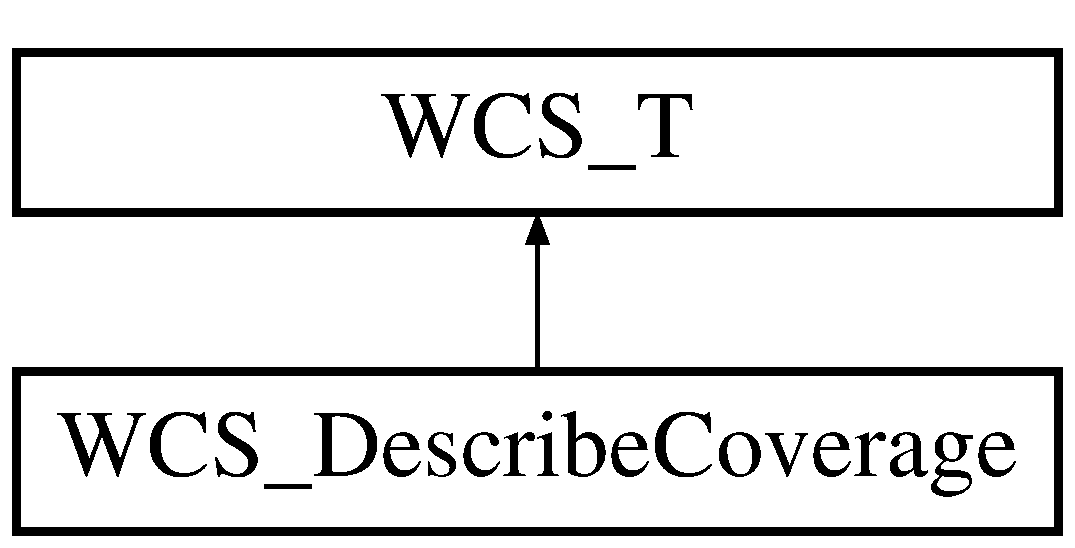
\includegraphics[height=2.000000cm]{classWCS__DescribeCoverage}
\end{center}
\end{figure}
\subsection*{Public Member Functions}
\begin{DoxyCompactItemize}
\item 
\hyperlink{classWCS__DescribeCoverage_a02b9cfa4a0ba1d6bf1f6f59da9be2742}{WCS\_\-DescribeCoverage} (const string \&conf)
\begin{DoxyCompactList}\small\item\em Constructor of a \hyperlink{classWCS__DescribeCoverage}{WCS\_\-DescribeCoverage} object. \end{DoxyCompactList}\item 
virtual CPLErr \hyperlink{classWCS__DescribeCoverage_aaa1f795a02b2b266e99302cef09fbd27}{GetReqMessageFromXMLTree} (CPLXMLNode $\ast$xmlRoot)
\begin{DoxyCompactList}\small\item\em Fetch the DescribeCoverage request parameters from XML tree object. \end{DoxyCompactList}\item 
virtual CPLErr \hyperlink{classWCS__DescribeCoverage_a68d2ceb47305263c78f9676e11ac7387}{GetReqMessageFromURLString} (const string \&)
\begin{DoxyCompactList}\small\item\em Fetch the request parameters from URL string. \end{DoxyCompactList}\item 
virtual void \hyperlink{classWCS__DescribeCoverage_a0c3bbc4bf7cd2ec6d469330d636c3390}{WCST\_\-Respond} (string \&sOutFileName)
\begin{DoxyCompactList}\small\item\em The enter point for \hyperlink{classWCS__DescribeCoverage}{WCS\_\-DescribeCoverage} class (Command line environment). \end{DoxyCompactList}\item 
virtual void \hyperlink{classWCS__DescribeCoverage_a6536fa20a925c8ce4b1d96f7e134e4ac}{WCST\_\-Respond} ()
\begin{DoxyCompactList}\small\item\em The enter point for \hyperlink{classWCS__DescribeCoverage}{WCS\_\-DescribeCoverage} class (CGI environment). \end{DoxyCompactList}\item 
void \hyperlink{classWCS__DescribeCoverage_ab007cc5bbbfa0d7e1707af408df27710}{CreateDescribeEOCoverageSetXMLHead} (ostringstream \&outStream)
\begin{DoxyCompactList}\small\item\em Create the XML head element for DescribeEOCoverageSet response. \end{DoxyCompactList}\item 
void \hyperlink{classWCS__DescribeCoverage_a385756678eac712ab993ac7a36d6c640}{CreateDescribeCoverageXMLHead} (ostringstream \&outStream)
\begin{DoxyCompactList}\small\item\em Create the XML head element for DescribeCoverage response. \end{DoxyCompactList}\item 
void \hyperlink{classWCS__DescribeCoverage_ab34c69c2877d1205e41b4d52c0c69ab8}{CreateOneCoverageDescription} (ostringstream \&outStream, \hyperlink{classDatasetObject}{DatasetObject} \&dsObj)
\begin{DoxyCompactList}\small\item\em Create the coverage description contents for the Dataset object. \end{DoxyCompactList}\item 
void \hyperlink{classWCS__DescribeCoverage_ae3f1103e9c8028ee5100c3c757c2f489}{CreateOneDatasetSeriesDescription} (ostringstream \&outStream, \hyperlink{classDatasetSeriesObject}{DatasetSeriesObject} \&dsSeriesObj)
\begin{DoxyCompactList}\small\item\em Create the coverage description contents for the DatasetSeries object. \end{DoxyCompactList}\item 
vector$<$ \hyperlink{classDatasetObject}{DatasetObject} $>$ \hyperlink{classWCS__DescribeCoverage_a33ceb7c235cfa5827444b7e27a1c72a9}{QueryFromDatasetSeries} (\hyperlink{classDatasetSeriesObject}{DatasetSeriesObject} \&dsSeriesObj)
\begin{DoxyCompactList}\small\item\em Query the dataset array from a datasetSeries object. \end{DoxyCompactList}\item 
CPLErr \hyperlink{classWCS__DescribeCoverage_ab5c7b3e04cbf771c2bcfb51d26d0c6ac}{CreateDescribeCoverageXMLTree} (ostringstream \&outStream)
\begin{DoxyCompactList}\small\item\em Create the whole response for DescribeCoverage or DescribeEOCoverageSet request. \end{DoxyCompactList}\end{DoxyCompactItemize}
\subsection*{Protected Attributes}
\begin{DoxyCompactItemize}
\item 
\hypertarget{classWCS__DescribeCoverage_a9003d4a2612ad19df154fdf86d28c12a}{
int {\bfseries mb\_\-DescribeEOCoverage}}
\label{classWCS__DescribeCoverage_a9003d4a2612ad19df154fdf86d28c12a}

\item 
\hypertarget{classWCS__DescribeCoverage_a27d51d8a1aa35146c3caa48b4ff1d788}{
int {\bfseries mB\_\-SubsetSpatialLat}}
\label{classWCS__DescribeCoverage_a27d51d8a1aa35146c3caa48b4ff1d788}

\item 
\hypertarget{classWCS__DescribeCoverage_a39a534b0be1be934dcfc1e13a619a479}{
int {\bfseries mB\_\-SubsetSpatialLon}}
\label{classWCS__DescribeCoverage_a39a534b0be1be934dcfc1e13a619a479}

\item 
\hypertarget{classWCS__DescribeCoverage_a1a3853ad442117bcde89bb6e5ee70476}{
int {\bfseries mB\_\-SubsetTemporalBegin}}
\label{classWCS__DescribeCoverage_a1a3853ad442117bcde89bb6e5ee70476}

\item 
\hypertarget{classWCS__DescribeCoverage_a777b37c1d93cedb87868e8160b484f72}{
int {\bfseries mB\_\-SubsetTemporalEnd}}
\label{classWCS__DescribeCoverage_a777b37c1d93cedb87868e8160b484f72}

\item 
\hypertarget{classWCS__DescribeCoverage_a38828e93877a6eb1fe2614ca24db8f36}{
double {\bfseries md\_\-RequestMinX}}
\label{classWCS__DescribeCoverage_a38828e93877a6eb1fe2614ca24db8f36}

\item 
\hypertarget{classWCS__DescribeCoverage_ae11ae1434f07b137d82ffff97c175f0f}{
double {\bfseries md\_\-RequestMaxX}}
\label{classWCS__DescribeCoverage_ae11ae1434f07b137d82ffff97c175f0f}

\item 
\hypertarget{classWCS__DescribeCoverage_a5140ec1a2f16699cbcfafdde54d789e9}{
double {\bfseries md\_\-RequestMinY}}
\label{classWCS__DescribeCoverage_a5140ec1a2f16699cbcfafdde54d789e9}

\item 
\hypertarget{classWCS__DescribeCoverage_a3ffada2c06820d2a05e496aaa5ff8c65}{
double {\bfseries md\_\-RequestMaxY}}
\label{classWCS__DescribeCoverage_a3ffada2c06820d2a05e496aaa5ff8c65}

\item 
\hypertarget{classWCS__DescribeCoverage_a8d7d1c3a7003594cfb31122e2a1c3a0a}{
string {\bfseries ms\_\-RequestBeginTime}}
\label{classWCS__DescribeCoverage_a8d7d1c3a7003594cfb31122e2a1c3a0a}

\item 
\hypertarget{classWCS__DescribeCoverage_a066dac63a3e2a2dbc7d1257f17ca1837}{
string {\bfseries ms\_\-RequestEndTime}}
\label{classWCS__DescribeCoverage_a066dac63a3e2a2dbc7d1257f17ca1837}

\item 
\hypertarget{classWCS__DescribeCoverage_a35432a1be89ef566f5b9538bdf185939}{
vector$<$ string $>$ {\bfseries mv\_\-CovIDs}}
\label{classWCS__DescribeCoverage_a35432a1be89ef566f5b9538bdf185939}

\end{DoxyCompactItemize}


\subsection{Detailed Description}
This class is used to handle DescribeCoverage and DescribeEOCoverageSet request. 

This class is used to handle DescribeCoverage and DescribeEOCoverageSet request. Several functions for parsing request parameters, generating the response XML document, are provided. 

\subsection{Constructor \& Destructor Documentation}
\hypertarget{classWCS__DescribeCoverage_a02b9cfa4a0ba1d6bf1f6f59da9be2742}{
\index{WCS\_\-DescribeCoverage@{WCS\_\-DescribeCoverage}!WCS\_\-DescribeCoverage@{WCS\_\-DescribeCoverage}}
\index{WCS\_\-DescribeCoverage@{WCS\_\-DescribeCoverage}!WCS_DescribeCoverage@{WCS\_\-DescribeCoverage}}
\subsubsection[{WCS\_\-DescribeCoverage}]{\setlength{\rightskip}{0pt plus 5cm}WCS\_\-DescribeCoverage::WCS\_\-DescribeCoverage (
\begin{DoxyParamCaption}
\item[{const string \&}]{conf}
\end{DoxyParamCaption}
)}}
\label{classWCS__DescribeCoverage_a02b9cfa4a0ba1d6bf1f6f59da9be2742}


Constructor of a \hyperlink{classWCS__DescribeCoverage}{WCS\_\-DescribeCoverage} object. 

This is the accepted method of creating an \hyperlink{classWCS__DescribeCoverage}{WCS\_\-DescribeCoverage} object.


\begin{DoxyParams}{Parameters}
{\em conf} & String of the full path of the configuration file. \\
\hline
\end{DoxyParams}


\subsection{Member Function Documentation}
\hypertarget{classWCS__DescribeCoverage_a385756678eac712ab993ac7a36d6c640}{
\index{WCS\_\-DescribeCoverage@{WCS\_\-DescribeCoverage}!CreateDescribeCoverageXMLHead@{CreateDescribeCoverageXMLHead}}
\index{CreateDescribeCoverageXMLHead@{CreateDescribeCoverageXMLHead}!WCS_DescribeCoverage@{WCS\_\-DescribeCoverage}}
\subsubsection[{CreateDescribeCoverageXMLHead}]{\setlength{\rightskip}{0pt plus 5cm}void WCS\_\-DescribeCoverage::CreateDescribeCoverageXMLHead (
\begin{DoxyParamCaption}
\item[{ostringstream \&}]{outStream}
\end{DoxyParamCaption}
)}}
\label{classWCS__DescribeCoverage_a385756678eac712ab993ac7a36d6c640}


Create the XML head element for DescribeCoverage response. 

This method is used to create the XML head element for DescribeCoverage response and append the response to the output stream.


\begin{DoxyParams}{Parameters}
{\em outStream} & Stream object used to generate DescribeCoverage response. \\
\hline
\end{DoxyParams}
\hypertarget{classWCS__DescribeCoverage_ab5c7b3e04cbf771c2bcfb51d26d0c6ac}{
\index{WCS\_\-DescribeCoverage@{WCS\_\-DescribeCoverage}!CreateDescribeCoverageXMLTree@{CreateDescribeCoverageXMLTree}}
\index{CreateDescribeCoverageXMLTree@{CreateDescribeCoverageXMLTree}!WCS_DescribeCoverage@{WCS\_\-DescribeCoverage}}
\subsubsection[{CreateDescribeCoverageXMLTree}]{\setlength{\rightskip}{0pt plus 5cm}CPLErr WCS\_\-DescribeCoverage::CreateDescribeCoverageXMLTree (
\begin{DoxyParamCaption}
\item[{ostringstream \&}]{outStream}
\end{DoxyParamCaption}
)}}
\label{classWCS__DescribeCoverage_ab5c7b3e04cbf771c2bcfb51d26d0c6ac}


Create the whole response for DescribeCoverage or DescribeEOCoverageSet request. 

This method is used to create the whole response for DescribeCoverage or DescribeEOCoverageSet request.


\begin{DoxyParams}{Parameters}
{\em outStream} & Stream object used to generate response.\\
\hline
\end{DoxyParams}
\begin{DoxyReturn}{Returns}
CE\_\-None on success or CE\_\-Failure on failure. 
\end{DoxyReturn}
\hypertarget{classWCS__DescribeCoverage_ab007cc5bbbfa0d7e1707af408df27710}{
\index{WCS\_\-DescribeCoverage@{WCS\_\-DescribeCoverage}!CreateDescribeEOCoverageSetXMLHead@{CreateDescribeEOCoverageSetXMLHead}}
\index{CreateDescribeEOCoverageSetXMLHead@{CreateDescribeEOCoverageSetXMLHead}!WCS_DescribeCoverage@{WCS\_\-DescribeCoverage}}
\subsubsection[{CreateDescribeEOCoverageSetXMLHead}]{\setlength{\rightskip}{0pt plus 5cm}void WCS\_\-DescribeCoverage::CreateDescribeEOCoverageSetXMLHead (
\begin{DoxyParamCaption}
\item[{ostringstream \&}]{outStream}
\end{DoxyParamCaption}
)}}
\label{classWCS__DescribeCoverage_ab007cc5bbbfa0d7e1707af408df27710}


Create the XML head element for DescribeEOCoverageSet response. 

This method is used to create the XML head element for DescribeEOCoverageSet response and append the response to the output stream.


\begin{DoxyParams}{Parameters}
{\em outStream} & Stream object used to generate DescribeEOCoverageSet response. \\
\hline
\end{DoxyParams}
\hypertarget{classWCS__DescribeCoverage_ab34c69c2877d1205e41b4d52c0c69ab8}{
\index{WCS\_\-DescribeCoverage@{WCS\_\-DescribeCoverage}!CreateOneCoverageDescription@{CreateOneCoverageDescription}}
\index{CreateOneCoverageDescription@{CreateOneCoverageDescription}!WCS_DescribeCoverage@{WCS\_\-DescribeCoverage}}
\subsubsection[{CreateOneCoverageDescription}]{\setlength{\rightskip}{0pt plus 5cm}void WCS\_\-DescribeCoverage::CreateOneCoverageDescription (
\begin{DoxyParamCaption}
\item[{ostringstream \&}]{outStream, }
\item[{{\bf DatasetObject} \&}]{dsObj}
\end{DoxyParamCaption}
)}}
\label{classWCS__DescribeCoverage_ab34c69c2877d1205e41b4d52c0c69ab8}


Create the coverage description contents for the Dataset object. 

This method is used to create the coverage description XMl elements for specified Dataset object, The generated XML element will be appended to the output stream.


\begin{DoxyParams}{Parameters}
{\em outStream} & Stream object used to generate response.\\
\hline
{\em dataset} & Dataset object which includes some attribute information about this dataset. \\
\hline
\end{DoxyParams}
\hypertarget{classWCS__DescribeCoverage_ae3f1103e9c8028ee5100c3c757c2f489}{
\index{WCS\_\-DescribeCoverage@{WCS\_\-DescribeCoverage}!CreateOneDatasetSeriesDescription@{CreateOneDatasetSeriesDescription}}
\index{CreateOneDatasetSeriesDescription@{CreateOneDatasetSeriesDescription}!WCS_DescribeCoverage@{WCS\_\-DescribeCoverage}}
\subsubsection[{CreateOneDatasetSeriesDescription}]{\setlength{\rightskip}{0pt plus 5cm}void WCS\_\-DescribeCoverage::CreateOneDatasetSeriesDescription (
\begin{DoxyParamCaption}
\item[{ostringstream \&}]{outStream, }
\item[{{\bf DatasetSeriesObject} \&}]{dsSeriesObj}
\end{DoxyParamCaption}
)}}
\label{classWCS__DescribeCoverage_ae3f1103e9c8028ee5100c3c757c2f489}


Create the coverage description contents for the DatasetSeries object. 

This method is used to create the coverage description XMl elements for specified DatasetSeries object, The generated XML element will be appended to the output stream.


\begin{DoxyParams}{Parameters}
{\em outStream} & Stream object used to generate response.\\
\hline
{\em dsSeriesObj} & DatasetSeries object which includes some attribute information about this datasetSeries. \\
\hline
\end{DoxyParams}
\hypertarget{classWCS__DescribeCoverage_a68d2ceb47305263c78f9676e11ac7387}{
\index{WCS\_\-DescribeCoverage@{WCS\_\-DescribeCoverage}!GetReqMessageFromURLString@{GetReqMessageFromURLString}}
\index{GetReqMessageFromURLString@{GetReqMessageFromURLString}!WCS_DescribeCoverage@{WCS\_\-DescribeCoverage}}
\subsubsection[{GetReqMessageFromURLString}]{\setlength{\rightskip}{0pt plus 5cm}CPLErr WCS\_\-DescribeCoverage::GetReqMessageFromURLString (
\begin{DoxyParamCaption}
\item[{const string \&}]{urlStr}
\end{DoxyParamCaption}
)\hspace{0.3cm}{\ttfamily  \mbox{[}virtual\mbox{]}}}}
\label{classWCS__DescribeCoverage_a68d2ceb47305263c78f9676e11ac7387}


Fetch the request parameters from URL string. 

This method is used to fetch the DescibeCoverage and DescribeEOCoverageSet parameters from an URL string (HTTP GET method). The coverage identifier(s) will be fetched.


\begin{DoxyParams}{Parameters}
{\em urlStr} & String of the DescibeCoverage or DescribeEOCoverageSet request.\\
\hline
\end{DoxyParams}
\begin{DoxyReturn}{Returns}
CE\_\-None on success or CE\_\-Failure on failure. 
\end{DoxyReturn}


Reimplemented from \hyperlink{classWCS__T}{WCS\_\-T}.

\hypertarget{classWCS__DescribeCoverage_aaa1f795a02b2b266e99302cef09fbd27}{
\index{WCS\_\-DescribeCoverage@{WCS\_\-DescribeCoverage}!GetReqMessageFromXMLTree@{GetReqMessageFromXMLTree}}
\index{GetReqMessageFromXMLTree@{GetReqMessageFromXMLTree}!WCS_DescribeCoverage@{WCS\_\-DescribeCoverage}}
\subsubsection[{GetReqMessageFromXMLTree}]{\setlength{\rightskip}{0pt plus 5cm}CPLErr WCS\_\-DescribeCoverage::GetReqMessageFromXMLTree (
\begin{DoxyParamCaption}
\item[{CPLXMLNode $\ast$}]{xmlRoot}
\end{DoxyParamCaption}
)\hspace{0.3cm}{\ttfamily  \mbox{[}virtual\mbox{]}}}}
\label{classWCS__DescribeCoverage_aaa1f795a02b2b266e99302cef09fbd27}


Fetch the DescribeCoverage request parameters from XML tree object. 

This method is used to fetch the DescibeCoverage and DescribeEOCoverageSet parameters from an XML object (HTTP POST method). The coverage identifier(s) will be fetched.

Sample request XML document 
\begin{DoxyCode}
<?xml version="1.0" encoding="UTF-8"?>
<DescribeCoverage
  xmlns:xsi="http://www.w3.org/2001/XMLSchema-instance"
  xmlns:wcs="http://www.opengis.net/wcs/2.0"
  xmlns:gml="http://www.opengis.net/gml/3.2"
  xsi:schemaLocation="http://schemas.opengis.net/wcs/2.0 ../wcsAll.xsd"
  service="WCS" version="2.0.0">
  <wcs:CoverageId>MOD05_L2.A2008205.0255.005.2008206170326.hdf:Water_Vapor_Infrar
      ed</wcs:CoverageId>
  <wcs:CoverageId>MOD13C1.A2007145.005.2007184062524.hdf:NDVI</wcs:CoverageId>
</DescribeCoverage>
\end{DoxyCode}



\begin{DoxyParams}{Parameters}
{\em xmlRoot} & XML Node object created by GDAL library.\\
\hline
\end{DoxyParams}
\begin{DoxyReturn}{Returns}
CE\_\-None on success or CE\_\-Failure on failure. 
\end{DoxyReturn}


Reimplemented from \hyperlink{classWCS__T}{WCS\_\-T}.

\hypertarget{classWCS__DescribeCoverage_a33ceb7c235cfa5827444b7e27a1c72a9}{
\index{WCS\_\-DescribeCoverage@{WCS\_\-DescribeCoverage}!QueryFromDatasetSeries@{QueryFromDatasetSeries}}
\index{QueryFromDatasetSeries@{QueryFromDatasetSeries}!WCS_DescribeCoverage@{WCS\_\-DescribeCoverage}}
\subsubsection[{QueryFromDatasetSeries}]{\setlength{\rightskip}{0pt plus 5cm}vector$<$ {\bf DatasetObject} $>$ WCS\_\-DescribeCoverage::QueryFromDatasetSeries (
\begin{DoxyParamCaption}
\item[{{\bf DatasetSeriesObject} \&}]{dso}
\end{DoxyParamCaption}
)}}
\label{classWCS__DescribeCoverage_a33ceb7c235cfa5827444b7e27a1c72a9}


Query the dataset array from a datasetSeries object. 

This method is used to query the dataset array from DatasetSeries object based on specified spatial-\/temporal parameters.


\begin{DoxyParams}{Parameters}
{\em dso} & DatasetSeries object.\\
\hline
\end{DoxyParams}
\begin{DoxyReturn}{Returns}
The array of result Dataset object. 
\end{DoxyReturn}
\hypertarget{classWCS__DescribeCoverage_a6536fa20a925c8ce4b1d96f7e134e4ac}{
\index{WCS\_\-DescribeCoverage@{WCS\_\-DescribeCoverage}!WCST\_\-Respond@{WCST\_\-Respond}}
\index{WCST\_\-Respond@{WCST\_\-Respond}!WCS_DescribeCoverage@{WCS\_\-DescribeCoverage}}
\subsubsection[{WCST\_\-Respond}]{\setlength{\rightskip}{0pt plus 5cm}void WCS\_\-DescribeCoverage::WCST\_\-Respond (
\begin{DoxyParamCaption}
{}
\end{DoxyParamCaption}
)\hspace{0.3cm}{\ttfamily  \mbox{[}virtual\mbox{]}}}}
\label{classWCS__DescribeCoverage_a6536fa20a925c8ce4b1d96f7e134e4ac}


The enter point for \hyperlink{classWCS__DescribeCoverage}{WCS\_\-DescribeCoverage} class (CGI environment). 

This method is the enter point for \hyperlink{classWCS__DescribeCoverage}{WCS\_\-DescribeCoverage} class, which is used under CGI environment. The response information will be displayed in the browser. 

Reimplemented from \hyperlink{classWCS__T}{WCS\_\-T}.

\hypertarget{classWCS__DescribeCoverage_a0c3bbc4bf7cd2ec6d469330d636c3390}{
\index{WCS\_\-DescribeCoverage@{WCS\_\-DescribeCoverage}!WCST\_\-Respond@{WCST\_\-Respond}}
\index{WCST\_\-Respond@{WCST\_\-Respond}!WCS_DescribeCoverage@{WCS\_\-DescribeCoverage}}
\subsubsection[{WCST\_\-Respond}]{\setlength{\rightskip}{0pt plus 5cm}void WCS\_\-DescribeCoverage::WCST\_\-Respond (
\begin{DoxyParamCaption}
\item[{string \&}]{sOutFileName}
\end{DoxyParamCaption}
)\hspace{0.3cm}{\ttfamily  \mbox{[}virtual\mbox{]}}}}
\label{classWCS__DescribeCoverage_a0c3bbc4bf7cd2ec6d469330d636c3390}


The enter point for \hyperlink{classWCS__DescribeCoverage}{WCS\_\-DescribeCoverage} class (Command line environment). 

This method is the enter point for \hyperlink{classWCS__DescribeCoverage}{WCS\_\-DescribeCoverage} class, which is used under command line environment. In order to debug WCS and use WCS as a command line, the user could issue a request under command line. The response information will be stored in the specified file.


\begin{DoxyParams}{Parameters}
{\em sOutFileName} & The path of the response file. \\
\hline
\end{DoxyParams}


Reimplemented from \hyperlink{classWCS__T}{WCS\_\-T}.



The documentation for this class was generated from the following files:\begin{DoxyCompactItemize}
\item 
WCS\_\-DescribeCoverage.h\item 
WCS\_\-DescribeCoverage.cpp\end{DoxyCompactItemize}

\hypertarget{classWCS__GetCapabilities}{
\section{WCS\_\-GetCapabilities Class Reference}
\label{classWCS__GetCapabilities}\index{WCS\_\-GetCapabilities@{WCS\_\-GetCapabilities}}
}


This class is used to handle GetCapabilities request.  




{\ttfamily \#include $<$WCS\_\-GetCapabilities.h$>$}

Inheritance diagram for WCS\_\-GetCapabilities:\begin{figure}[H]
\begin{center}
\leavevmode
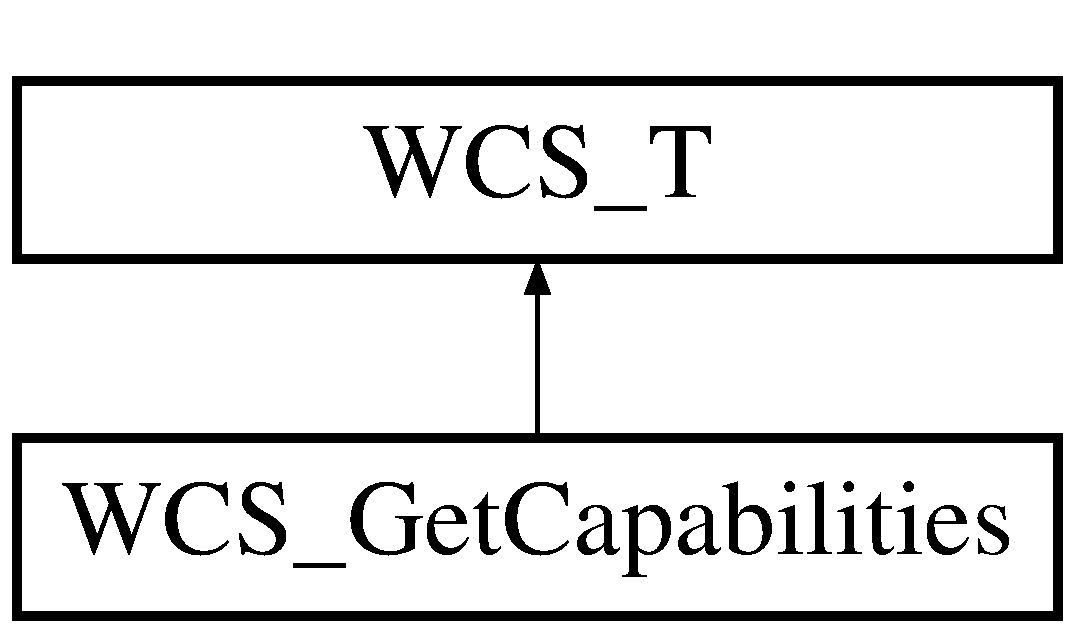
\includegraphics[height=2.000000cm]{classWCS__GetCapabilities}
\end{center}
\end{figure}
\subsection*{Public Member Functions}
\begin{DoxyCompactItemize}
\item 
\hyperlink{classWCS__GetCapabilities_a305c85654f218ad2e30e763b0e173cb1}{WCS\_\-GetCapabilities} (const string \&conf)
\begin{DoxyCompactList}\small\item\em Constructor of a \hyperlink{classWCS__GetCapabilities}{WCS\_\-GetCapabilities} object. \end{DoxyCompactList}\item 
virtual CPLErr \hyperlink{classWCS__GetCapabilities_ad640c177b1cc20859640090adc608d3e}{GetReqMessageFromXMLTree} (CPLXMLNode $\ast$xmlRoot)
\begin{DoxyCompactList}\small\item\em Fetch the request GetCapabilities parameters from XML tree object. \end{DoxyCompactList}\item 
virtual CPLErr \hyperlink{classWCS__GetCapabilities_a5e0c27a53f396893afd5f796e7c38ee0}{GetReqMessageFromURLString} (const string \&)
\begin{DoxyCompactList}\small\item\em Fetch the request parameters from URL string. \end{DoxyCompactList}\item 
virtual void \hyperlink{classWCS__GetCapabilities_a5da60bec7f2ebce37b1acbcea547cf1d}{WCST\_\-Respond} (string \&sOutFileName)
\begin{DoxyCompactList}\small\item\em The enter point for \hyperlink{classWCS__GetCapabilities}{WCS\_\-GetCapabilities} class (Command line environment). \end{DoxyCompactList}\item 
virtual void \hyperlink{classWCS__GetCapabilities_af250d7ecba600be323a1eb6778bdd4e7}{WCST\_\-Respond} ()
\begin{DoxyCompactList}\small\item\em The enter point for \hyperlink{classWCS__GetCapabilities}{WCS\_\-GetCapabilities} class (CGI environment). \end{DoxyCompactList}\end{DoxyCompactItemize}
\subsection*{Protected Attributes}
\begin{DoxyCompactItemize}
\item 
\hypertarget{classWCS__GetCapabilities_a3ffc84e44c2bad1dc5cf048d9c787719}{
vector$<$ string $>$ {\bfseries mv\_\-sections}}
\label{classWCS__GetCapabilities_a3ffc84e44c2bad1dc5cf048d9c787719}

\end{DoxyCompactItemize}


\subsection{Detailed Description}
This class is used to handle GetCapabilities request. 

This class is used to handle GetCapabilities request. Several functions for parsing request parameters, generating the response XML document, are provided. 

\subsection{Constructor \& Destructor Documentation}
\hypertarget{classWCS__GetCapabilities_a305c85654f218ad2e30e763b0e173cb1}{
\index{WCS\_\-GetCapabilities@{WCS\_\-GetCapabilities}!WCS\_\-GetCapabilities@{WCS\_\-GetCapabilities}}
\index{WCS\_\-GetCapabilities@{WCS\_\-GetCapabilities}!WCS_GetCapabilities@{WCS\_\-GetCapabilities}}
\subsubsection[{WCS\_\-GetCapabilities}]{\setlength{\rightskip}{0pt plus 5cm}WCS\_\-GetCapabilities::WCS\_\-GetCapabilities (
\begin{DoxyParamCaption}
\item[{const string \&}]{conf}
\end{DoxyParamCaption}
)}}
\label{classWCS__GetCapabilities_a305c85654f218ad2e30e763b0e173cb1}


Constructor of a \hyperlink{classWCS__GetCapabilities}{WCS\_\-GetCapabilities} object. 

This is the accepted method of creating an \hyperlink{classWCS__GetCapabilities}{WCS\_\-GetCapabilities} object.


\begin{DoxyParams}{Parameters}
{\em conf} & String of the full path of the configuration file. \\
\hline
\end{DoxyParams}


\subsection{Member Function Documentation}
\hypertarget{classWCS__GetCapabilities_a5e0c27a53f396893afd5f796e7c38ee0}{
\index{WCS\_\-GetCapabilities@{WCS\_\-GetCapabilities}!GetReqMessageFromURLString@{GetReqMessageFromURLString}}
\index{GetReqMessageFromURLString@{GetReqMessageFromURLString}!WCS_GetCapabilities@{WCS\_\-GetCapabilities}}
\subsubsection[{GetReqMessageFromURLString}]{\setlength{\rightskip}{0pt plus 5cm}CPLErr WCS\_\-GetCapabilities::GetReqMessageFromURLString (
\begin{DoxyParamCaption}
\item[{const string \&}]{urlStr}
\end{DoxyParamCaption}
)\hspace{0.3cm}{\ttfamily  \mbox{[}virtual\mbox{]}}}}
\label{classWCS__GetCapabilities_a5e0c27a53f396893afd5f796e7c38ee0}


Fetch the request parameters from URL string. 

This method is used to fetch the GetCapabilities parameters from an URL string (HTTP GET method).


\begin{DoxyParams}{Parameters}
{\em urlStr} & String of the GetCapabilities request.\\
\hline
\end{DoxyParams}
\begin{DoxyReturn}{Returns}
CE\_\-None on success or CE\_\-Failure on failure. 
\end{DoxyReturn}


Reimplemented from \hyperlink{classWCS__T}{WCS\_\-T}.

\hypertarget{classWCS__GetCapabilities_ad640c177b1cc20859640090adc608d3e}{
\index{WCS\_\-GetCapabilities@{WCS\_\-GetCapabilities}!GetReqMessageFromXMLTree@{GetReqMessageFromXMLTree}}
\index{GetReqMessageFromXMLTree@{GetReqMessageFromXMLTree}!WCS_GetCapabilities@{WCS\_\-GetCapabilities}}
\subsubsection[{GetReqMessageFromXMLTree}]{\setlength{\rightskip}{0pt plus 5cm}CPLErr WCS\_\-GetCapabilities::GetReqMessageFromXMLTree (
\begin{DoxyParamCaption}
\item[{CPLXMLNode $\ast$}]{xmlRoot}
\end{DoxyParamCaption}
)\hspace{0.3cm}{\ttfamily  \mbox{[}virtual\mbox{]}}}}
\label{classWCS__GetCapabilities_ad640c177b1cc20859640090adc608d3e}


Fetch the request GetCapabilities parameters from XML tree object. 

This method is used to fetch the GetCapabilities parameters from an XML object (HTTP POST method).

Sample request XML document 
\begin{DoxyCode}
<?xml version="1.0" encoding="UTF-8"?>
<GetCapabilities
  xmlns:xsi="http://www.w3.org/2001/XMLSchema-instance"
  xmlns:ows="http://www.opengis.net/ows/1.1"
  xmlns:wcs="http://www.opengis.net/wcs/2.0"
  xsi:schemaLocation=
    "http://schemas.opengis.net/wcs/2.0 ../wcsAll.xsd"
  service="WCS">
  <ows:AcceptVersions>
    <ows:Version>2.0.0</ows:Version>
  </ows:AcceptVersions>
</GetCapabilities>
\end{DoxyCode}



\begin{DoxyParams}{Parameters}
{\em xmlRoot} & XML Node object created by GDAL library.\\
\hline
\end{DoxyParams}
\begin{DoxyReturn}{Returns}
CE\_\-None on success or CE\_\-Failure on failure. 
\end{DoxyReturn}


Reimplemented from \hyperlink{classWCS__T}{WCS\_\-T}.

\hypertarget{classWCS__GetCapabilities_a5da60bec7f2ebce37b1acbcea547cf1d}{
\index{WCS\_\-GetCapabilities@{WCS\_\-GetCapabilities}!WCST\_\-Respond@{WCST\_\-Respond}}
\index{WCST\_\-Respond@{WCST\_\-Respond}!WCS_GetCapabilities@{WCS\_\-GetCapabilities}}
\subsubsection[{WCST\_\-Respond}]{\setlength{\rightskip}{0pt plus 5cm}void WCS\_\-GetCapabilities::WCST\_\-Respond (
\begin{DoxyParamCaption}
\item[{string \&}]{sOutFileName}
\end{DoxyParamCaption}
)\hspace{0.3cm}{\ttfamily  \mbox{[}virtual\mbox{]}}}}
\label{classWCS__GetCapabilities_a5da60bec7f2ebce37b1acbcea547cf1d}


The enter point for \hyperlink{classWCS__GetCapabilities}{WCS\_\-GetCapabilities} class (Command line environment). 

This method is the enter point for \hyperlink{classWCS__GetCapabilities}{WCS\_\-GetCapabilities} class, which is used under command line environment. In order to debug WCS and use WCS as a command line, the user could issue a request under command line. The response information will be stored in the specified file.


\begin{DoxyParams}{Parameters}
{\em sOutFileName} & The path of the response file. \\
\hline
\end{DoxyParams}


Reimplemented from \hyperlink{classWCS__T}{WCS\_\-T}.

\hypertarget{classWCS__GetCapabilities_af250d7ecba600be323a1eb6778bdd4e7}{
\index{WCS\_\-GetCapabilities@{WCS\_\-GetCapabilities}!WCST\_\-Respond@{WCST\_\-Respond}}
\index{WCST\_\-Respond@{WCST\_\-Respond}!WCS_GetCapabilities@{WCS\_\-GetCapabilities}}
\subsubsection[{WCST\_\-Respond}]{\setlength{\rightskip}{0pt plus 5cm}void WCS\_\-GetCapabilities::WCST\_\-Respond (
\begin{DoxyParamCaption}
{}
\end{DoxyParamCaption}
)\hspace{0.3cm}{\ttfamily  \mbox{[}virtual\mbox{]}}}}
\label{classWCS__GetCapabilities_af250d7ecba600be323a1eb6778bdd4e7}


The enter point for \hyperlink{classWCS__GetCapabilities}{WCS\_\-GetCapabilities} class (CGI environment). 

This method is the enter point for \hyperlink{classWCS__GetCapabilities}{WCS\_\-GetCapabilities} class, which is used under CGI environment. The response information will be displayed in the browser. 

Reimplemented from \hyperlink{classWCS__T}{WCS\_\-T}.



The documentation for this class was generated from the following files:\begin{DoxyCompactItemize}
\item 
WCS\_\-GetCapabilities.h\item 
WCS\_\-GetCapabilities.cpp\end{DoxyCompactItemize}

\hypertarget{classWCS__GetCoverage}{
\section{WCS\_\-GetCoverage Class Reference}
\label{classWCS__GetCoverage}\index{WCS\_\-GetCoverage@{WCS\_\-GetCoverage}}
}


This class is used to handle GetCoverage request.  




{\ttfamily \#include $<$WCS\_\-GetCoverage.h$>$}

Inheritance diagram for WCS\_\-GetCoverage:\begin{figure}[H]
\begin{center}
\leavevmode
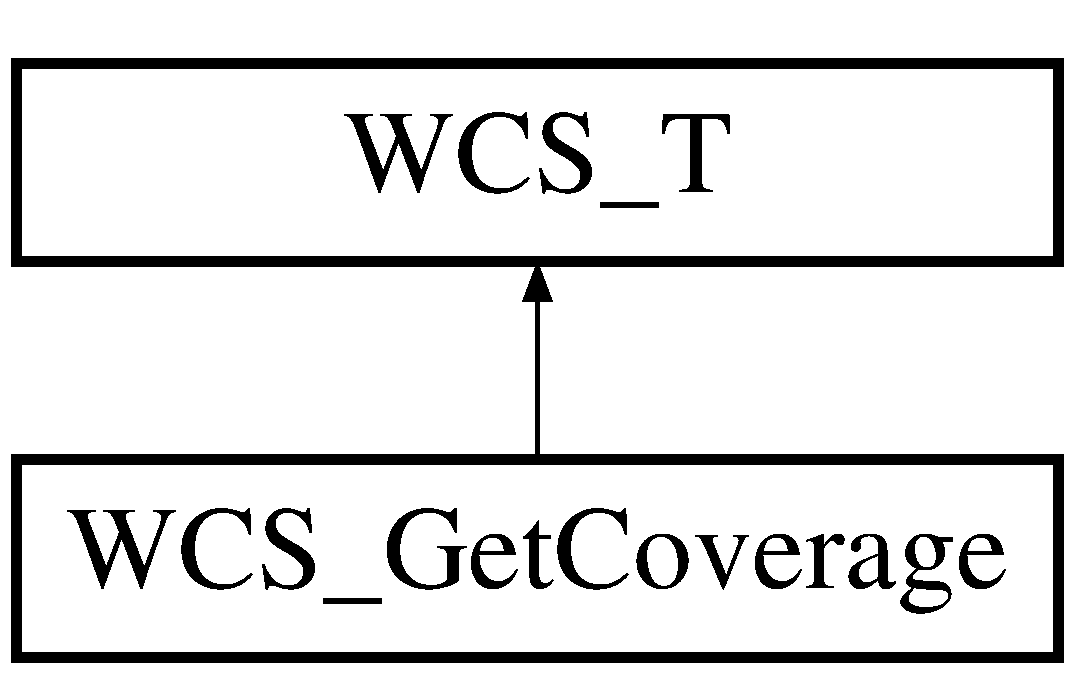
\includegraphics[height=2.000000cm]{classWCS__GetCoverage}
\end{center}
\end{figure}
\subsection*{Public Member Functions}
\begin{DoxyCompactItemize}
\item 
\hyperlink{classWCS__GetCoverage_a2bc572e0a90baf87f5d572d29db7e32e}{WCS\_\-GetCoverage} (const string \&conf)
\begin{DoxyCompactList}\small\item\em Constructor of a \hyperlink{classWCS__GetCoverage}{WCS\_\-GetCoverage} object. \end{DoxyCompactList}\item 
virtual CPLErr \hyperlink{classWCS__GetCoverage_a1a23003ebbaef4915fdc88863abf987c}{GetReqMessageFromXMLTree} (CPLXMLNode $\ast$xmlRoot)
\begin{DoxyCompactList}\small\item\em Fetch the \hyperlink{classWCS__GetCoverage}{WCS\_\-GetCoverage} request parameters from XML tree object. \end{DoxyCompactList}\item 
virtual CPLErr \hyperlink{classWCS__GetCoverage_aff25c578374abc386dc1455990198276}{GetReqMessageFromURLString} (const string \&)
\begin{DoxyCompactList}\small\item\em Fetch the request parameters from URL string. \end{DoxyCompactList}\item 
\hypertarget{classWCS__GetCoverage_aa5828099182998b05b50418161d01c8d}{
virtual void {\bfseries SetSoapMessage} (const int \&soapMsg)}
\label{classWCS__GetCoverage_aa5828099182998b05b50418161d01c8d}

\item 
\hypertarget{classWCS__GetCoverage_a2091115ee1479ddef8071f8fca80cf6b}{
virtual int {\bfseries IsSoapRequested} ()}
\label{classWCS__GetCoverage_a2091115ee1479ddef8071f8fca80cf6b}

\item 
virtual void \hyperlink{classWCS__GetCoverage_ad6d663aa5cd34f1cfeec96a8aa67fe6d}{WCST\_\-Respond} (string \&sOutFileName)
\begin{DoxyCompactList}\small\item\em The enter point for \hyperlink{classWCS__GetCoverage}{WCS\_\-GetCoverage} class (Command line environment). \end{DoxyCompactList}\item 
virtual void \hyperlink{classWCS__GetCoverage_ad8123a3ce047ab51e943bec28c6bca02}{WCST\_\-Respond} ()
\begin{DoxyCompactList}\small\item\em The enter point for \hyperlink{classWCS__GetCoverage}{WCS\_\-GetCoverage} class (CGI environment). \end{DoxyCompactList}\end{DoxyCompactItemize}
\subsection*{Protected Member Functions}
\begin{DoxyCompactItemize}
\item 
string \hyperlink{classWCS__GetCoverage_af70345de7d0cd908c28d9008d73569bf}{CreateOutputFileSuffix} ()
\begin{DoxyCompactList}\small\item\em Create the output suffix corresponding specified format. \end{DoxyCompactList}\item 
CPLErr \hyperlink{classWCS__GetCoverage_a0b4bdb2cf27cf85bea24529215daa372}{CreateISO19115Metadata} (\hyperlink{classDatasetObject}{DatasetObject} dsObj)
\begin{DoxyCompactList}\small\item\em Create an XML document following ISO 19115 and ISO 19115-\/2 standards. \end{DoxyCompactList}\item 
CPLErr \hyperlink{classWCS__GetCoverage_a1ef04fe1f8036a6347167b05eaaaa674}{CreateEOMetadata} (const string \&sOutFileName)
\begin{DoxyCompactList}\small\item\em Create an EO metadata for the output. \end{DoxyCompactList}\item 
CPLErr \hyperlink{classWCS__GetCoverage_a2b1cb91bae3d6cd3098d74ac666d557d}{GetCoverageInitial} ()
\begin{DoxyCompactList}\small\item\em Initialize the coverage object. \end{DoxyCompactList}\item 
CPLErr \hyperlink{classWCS__GetCoverage_a907d391b5e85ec4d3ca17316f69d3be0}{SetCRSFromURN} (OGRSpatialReference \&crs\_\-ID, const char $\ast$CRS\_\-urn)
\begin{DoxyCompactList}\small\item\em Set the OGRSpatialReference object based on CRS code. \end{DoxyCompactList}\item 
CPLErr \hyperlink{classWCS__GetCoverage_af624f4a8cac34ccd1bd16bbd67a685be}{CreateBinaryFile} (const string \&sOutFileName)
\begin{DoxyCompactList}\small\item\em Create the file in binary stream. \end{DoxyCompactList}\item 
\hypertarget{classWCS__GetCoverage_af3b045ddefc1f5859e85234674a4b813}{
CPLErr {\bfseries CreateHDFEOS2File} (const string \&sSourceFile, string hdfeosFile)}
\label{classWCS__GetCoverage_af3b045ddefc1f5859e85234674a4b813}

\item 
CPLErr \hyperlink{classWCS__GetCoverage_a38ebb99c11736874a5fdf9898aa3ce7f}{CreateOutputFile} (const string \&sOutFileName)
\begin{DoxyCompactList}\small\item\em Create the output file. \end{DoxyCompactList}\item 
CPLErr \hyperlink{classWCS__GetCoverage_a32d3c6edbb677534e0036c4acb6a327c}{SetOutputResolution} ()
\begin{DoxyCompactList}\small\item\em Set the output resolution based on specified resolution or width/height. \end{DoxyCompactList}\item 
CPLErr \hyperlink{classWCS__GetCoverage_a890b915a63bc56d6057981527d3f680e}{HttpDirectoryRespond} (const string \&sOutFileName)
\begin{DoxyCompactList}\small\item\em Delivery the output file stream to user directly. \end{DoxyCompactList}\item 
CPLErr \hyperlink{classWCS__GetCoverage_a1e8c186ce55e8f06e60681334dd38715}{HttpStoreRespond} (const string \&sOutFileName)
\begin{DoxyCompactList}\small\item\em Delivery the output file URL to user. \end{DoxyCompactList}\item 
CPLErr \hyperlink{classWCS__GetCoverage_aed557090f7ea436d261959393f878e32}{HttpMultiPartsDirectoryRespond} (const string \&sOutFileName)
\begin{DoxyCompactList}\small\item\em Delivery the output file stream to user and the metadata to browser. \end{DoxyCompactList}\item 
CPLErr \hyperlink{classWCS__GetCoverage_a3d3409267ed54560783523097a75f966}{ExeCommand} (string logFilePath, string cmd)
\begin{DoxyCompactList}\small\item\em Execute the command line by calling system function. \end{DoxyCompactList}\end{DoxyCompactItemize}
\subsection*{Protected Attributes}
\begin{DoxyCompactItemize}
\item 
\hypertarget{classWCS__GetCoverage_a0b020807d7c60cdaf046d44d3edce819}{
auto\_\-ptr$<$ \hyperlink{classAbstractDataset}{AbstractDataset} $>$ {\bfseries mp\_\-AbsDS}}
\label{classWCS__GetCoverage_a0b020807d7c60cdaf046d44d3edce819}

\item 
\hypertarget{classWCS__GetCoverage_aca3c07c25bff3602c7e40013975ee35e}{
double {\bfseries md\_\-RequestMinX}}
\label{classWCS__GetCoverage_aca3c07c25bff3602c7e40013975ee35e}

\item 
\hypertarget{classWCS__GetCoverage_a1fce35d813d5d03123ceba262e08e17f}{
double {\bfseries md\_\-RequestMinY}}
\label{classWCS__GetCoverage_a1fce35d813d5d03123ceba262e08e17f}

\item 
\hypertarget{classWCS__GetCoverage_a7be6a006f5e415b000e414c679ddc3fa}{
double {\bfseries md\_\-RequestMaxX}}
\label{classWCS__GetCoverage_a7be6a006f5e415b000e414c679ddc3fa}

\item 
\hypertarget{classWCS__GetCoverage_af59dd0be9bf9071e728566f188f340a2}{
double {\bfseries md\_\-RequestMaxY}}
\label{classWCS__GetCoverage_af59dd0be9bf9071e728566f188f340a2}

\item 
\hypertarget{classWCS__GetCoverage_a3bfddcafea9a4e37a5c9b907cdb22f05}{
int {\bfseries mi\_\-OutputWidth}}
\label{classWCS__GetCoverage_a3bfddcafea9a4e37a5c9b907cdb22f05}

\item 
\hypertarget{classWCS__GetCoverage_a983a30695a9383899f37e6122a256707}{
int {\bfseries mi\_\-OutputHeight}}
\label{classWCS__GetCoverage_a983a30695a9383899f37e6122a256707}

\item 
\hypertarget{classWCS__GetCoverage_a9af081fe2292169313de72854de2ae65}{
vector$<$ int $>$ {\bfseries mvi\_\-OutputWH}}
\label{classWCS__GetCoverage_a9af081fe2292169313de72854de2ae65}

\item 
\hypertarget{classWCS__GetCoverage_a35d80545e0d1c13ba2a87e047a8ff46c}{
vector$<$ double $>$ {\bfseries mvd\_\-OutputResXY}}
\label{classWCS__GetCoverage_a35d80545e0d1c13ba2a87e047a8ff46c}

\item 
\hypertarget{classWCS__GetCoverage_a829197779be16e6f042be3efcb0076f5}{
string {\bfseries ms\_\-CovID}}
\label{classWCS__GetCoverage_a829197779be16e6f042be3efcb0076f5}

\item 
\hypertarget{classWCS__GetCoverage_a1d630f3a3f415a4bf69cda05748bd119}{
string {\bfseries ms\_\-CovGDALID}}
\label{classWCS__GetCoverage_a1d630f3a3f415a4bf69cda05748bd119}

\item 
\hypertarget{classWCS__GetCoverage_ac9fdb17263aa227ca78dca3fad7c8dd9}{
string {\bfseries ms\_\-RequestCRS\_\-URN}}
\label{classWCS__GetCoverage_ac9fdb17263aa227ca78dca3fad7c8dd9}

\item 
\hypertarget{classWCS__GetCoverage_afc537ff82939218286269ce8ba50446d}{
string {\bfseries ms\_\-ResponseCRS\_\-URN}}
\label{classWCS__GetCoverage_afc537ff82939218286269ce8ba50446d}

\item 
\hypertarget{classWCS__GetCoverage_a2d654c6172b5ed16ae6fc9439a8131e8}{
string {\bfseries ms\_\-OutputFormat}}
\label{classWCS__GetCoverage_a2d654c6172b5ed16ae6fc9439a8131e8}

\item 
\hypertarget{classWCS__GetCoverage_a85a1fdbc04a32a3c8fb64bad27cfa94d}{
string {\bfseries ms\_\-OutputFormatCode}}
\label{classWCS__GetCoverage_a85a1fdbc04a32a3c8fb64bad27cfa94d}

\item 
\hypertarget{classWCS__GetCoverage_ad47ad94e7acd9cc7e53befaaef5a14bb}{
string {\bfseries ms\_\-OutputContentType}}
\label{classWCS__GetCoverage_ad47ad94e7acd9cc7e53befaaef5a14bb}

\item 
\hypertarget{classWCS__GetCoverage_acf98719a81dc740af138f8df7c71d5c3}{
string {\bfseries ms\_\-RequestBeginTime}}
\label{classWCS__GetCoverage_acf98719a81dc740af138f8df7c71d5c3}

\item 
\hypertarget{classWCS__GetCoverage_aec61f2f3ec14e51f8592fe692b7dcd1b}{
string {\bfseries ms\_\-RequestEndTime}}
\label{classWCS__GetCoverage_aec61f2f3ec14e51f8592fe692b7dcd1b}

\item 
\hypertarget{classWCS__GetCoverage_abf29f4df2c170376a2dcbebe4f38dc2b}{
string {\bfseries ms\_\-Interpolation}}
\label{classWCS__GetCoverage_abf29f4df2c170376a2dcbebe4f38dc2b}

\item 
\hypertarget{classWCS__GetCoverage_a2b325ed109ae7b9578a4ea92d1a85b01}{
int {\bfseries mb\_\-IsStore}}
\label{classWCS__GetCoverage_a2b325ed109ae7b9578a4ea92d1a85b01}

\item 
\hypertarget{classWCS__GetCoverage_a6ff57c181b18c4f56d14178d83f25d52}{
int {\bfseries mb\_\-SubsetSpatial}}
\label{classWCS__GetCoverage_a6ff57c181b18c4f56d14178d83f25d52}

\item 
\hypertarget{classWCS__GetCoverage_acadd942be00df0c80ad95f8eddec19ff}{
int {\bfseries mb\_\-MultiPart}}
\label{classWCS__GetCoverage_acadd942be00df0c80ad95f8eddec19ff}

\item 
\hypertarget{classWCS__GetCoverage_a5f1b0349f1e4977ae38110749590e709}{
OGRSpatialReference {\bfseries mo\_\-NativeCRS}}
\label{classWCS__GetCoverage_a5f1b0349f1e4977ae38110749590e709}

\item 
\hypertarget{classWCS__GetCoverage_adbe146d4c5abcbd811772e22e2712b9b}{
OGRSpatialReference {\bfseries mo\_\-RequestedCRS}}
\label{classWCS__GetCoverage_adbe146d4c5abcbd811772e22e2712b9b}

\item 
\hypertarget{classWCS__GetCoverage_aa2af672aaf0d65ef46d6edc067486170}{
OGRSpatialReference {\bfseries mo\_\-ResponseCRS}}
\label{classWCS__GetCoverage_aa2af672aaf0d65ef46d6edc067486170}

\item 
\hypertarget{classWCS__GetCoverage_aff40bdde8e489d0647d07d0c1342dcae}{
vector$<$ int $>$ {\bfseries mvi\_\-BandList}}
\label{classWCS__GetCoverage_aff40bdde8e489d0647d07d0c1342dcae}

\item 
\hypertarget{classWCS__GetCoverage_aa7873d69344c6495a7a72655c753e48f}{
double {\bfseries md\_\-OutGeoTransform} \mbox{[}6\mbox{]}}
\label{classWCS__GetCoverage_aa7873d69344c6495a7a72655c753e48f}

\item 
\hypertarget{classWCS__GetCoverage_a28b6f3ae72b3a62e0841375395200518}{
GDALResampleAlg {\bfseries me\_\-Interplation}}
\label{classWCS__GetCoverage_a28b6f3ae72b3a62e0841375395200518}

\end{DoxyCompactItemize}


\subsection{Detailed Description}
This class is used to handle GetCoverage request. 

This class is used to handle GetCoverage request. Several functions for parsing request parameters, generating the response file, are provided. 

\subsection{Constructor \& Destructor Documentation}
\hypertarget{classWCS__GetCoverage_a2bc572e0a90baf87f5d572d29db7e32e}{
\index{WCS\_\-GetCoverage@{WCS\_\-GetCoverage}!WCS\_\-GetCoverage@{WCS\_\-GetCoverage}}
\index{WCS\_\-GetCoverage@{WCS\_\-GetCoverage}!WCS_GetCoverage@{WCS\_\-GetCoverage}}
\subsubsection[{WCS\_\-GetCoverage}]{\setlength{\rightskip}{0pt plus 5cm}WCS\_\-GetCoverage::WCS\_\-GetCoverage (
\begin{DoxyParamCaption}
\item[{const string \&}]{conf}
\end{DoxyParamCaption}
)}}
\label{classWCS__GetCoverage_a2bc572e0a90baf87f5d572d29db7e32e}


Constructor of a \hyperlink{classWCS__GetCoverage}{WCS\_\-GetCoverage} object. 

This is the accepted method of creating an \hyperlink{classWCS__GetCoverage}{WCS\_\-GetCoverage} object.


\begin{DoxyParams}{Parameters}
{\em conf} & String of the full path of the configuration file. \\
\hline
\end{DoxyParams}


\subsection{Member Function Documentation}
\hypertarget{classWCS__GetCoverage_af624f4a8cac34ccd1bd16bbd67a685be}{
\index{WCS\_\-GetCoverage@{WCS\_\-GetCoverage}!CreateBinaryFile@{CreateBinaryFile}}
\index{CreateBinaryFile@{CreateBinaryFile}!WCS_GetCoverage@{WCS\_\-GetCoverage}}
\subsubsection[{CreateBinaryFile}]{\setlength{\rightskip}{0pt plus 5cm}CPLErr WCS\_\-GetCoverage::CreateBinaryFile (
\begin{DoxyParamCaption}
\item[{const string \&}]{sOutFileName}
\end{DoxyParamCaption}
)\hspace{0.3cm}{\ttfamily  \mbox{[}protected\mbox{]}}}}
\label{classWCS__GetCoverage_af624f4a8cac34ccd1bd16bbd67a685be}


Create the file in binary stream. 

This method is used to create the file in binary stream.

\begin{DoxyReturn}{Returns}
CE\_\-None on success or CE\_\-Failure on failure. 
\end{DoxyReturn}
\hypertarget{classWCS__GetCoverage_a1ef04fe1f8036a6347167b05eaaaa674}{
\index{WCS\_\-GetCoverage@{WCS\_\-GetCoverage}!CreateEOMetadata@{CreateEOMetadata}}
\index{CreateEOMetadata@{CreateEOMetadata}!WCS_GetCoverage@{WCS\_\-GetCoverage}}
\subsubsection[{CreateEOMetadata}]{\setlength{\rightskip}{0pt plus 5cm}CPLErr WCS\_\-GetCoverage::CreateEOMetadata (
\begin{DoxyParamCaption}
\item[{const string \&}]{sOutFileName}
\end{DoxyParamCaption}
)\hspace{0.3cm}{\ttfamily  \mbox{[}protected\mbox{]}}}}
\label{classWCS__GetCoverage_a1ef04fe1f8036a6347167b05eaaaa674}


Create an EO metadata for the output. 

This method is used to create ann EO metadata for the output.


\begin{DoxyParams}{Parameters}
{\em sOutFileName} & The path of output file.\\
\hline
\end{DoxyParams}
\begin{DoxyReturn}{Returns}
CE\_\-None on success or CE\_\-Failure on failure. 
\end{DoxyReturn}
\hypertarget{classWCS__GetCoverage_a0b4bdb2cf27cf85bea24529215daa372}{
\index{WCS\_\-GetCoverage@{WCS\_\-GetCoverage}!CreateISO19115Metadata@{CreateISO19115Metadata}}
\index{CreateISO19115Metadata@{CreateISO19115Metadata}!WCS_GetCoverage@{WCS\_\-GetCoverage}}
\subsubsection[{CreateISO19115Metadata}]{\setlength{\rightskip}{0pt plus 5cm}CPLErr WCS\_\-GetCoverage::CreateISO19115Metadata (
\begin{DoxyParamCaption}
\item[{{\bf DatasetObject}}]{dsObj}
\end{DoxyParamCaption}
)\hspace{0.3cm}{\ttfamily  \mbox{[}protected\mbox{]}}}}
\label{classWCS__GetCoverage_a0b4bdb2cf27cf85bea24529215daa372}


Create an XML document following ISO 19115 and ISO 19115-\/2 standards. 

This method is used to create an XML document following ISO 19115 and ISO 19115-\/2 standards, which is based on specified dataset object. There is a template file which is available through configuration file. After reading the template to memory, some keywords will be replace based on specified dataset object.


\begin{DoxyParams}{Parameters}
{\em dsObj} & Dataset object.\\
\hline
\end{DoxyParams}
\begin{DoxyReturn}{Returns}
CE\_\-None on success or CE\_\-Failure on failure. 
\end{DoxyReturn}
\hypertarget{classWCS__GetCoverage_a38ebb99c11736874a5fdf9898aa3ce7f}{
\index{WCS\_\-GetCoverage@{WCS\_\-GetCoverage}!CreateOutputFile@{CreateOutputFile}}
\index{CreateOutputFile@{CreateOutputFile}!WCS_GetCoverage@{WCS\_\-GetCoverage}}
\subsubsection[{CreateOutputFile}]{\setlength{\rightskip}{0pt plus 5cm}CPLErr WCS\_\-GetCoverage::CreateOutputFile (
\begin{DoxyParamCaption}
\item[{const string \&}]{sOutFileName}
\end{DoxyParamCaption}
)\hspace{0.3cm}{\ttfamily  \mbox{[}protected\mbox{]}}}}
\label{classWCS__GetCoverage_a38ebb99c11736874a5fdf9898aa3ce7f}


Create the output file. 

This method is used to create the output file.

\begin{DoxyReturn}{Returns}
CE\_\-None on success or CE\_\-Failure on failure. 
\end{DoxyReturn}
\hypertarget{classWCS__GetCoverage_af70345de7d0cd908c28d9008d73569bf}{
\index{WCS\_\-GetCoverage@{WCS\_\-GetCoverage}!CreateOutputFileSuffix@{CreateOutputFileSuffix}}
\index{CreateOutputFileSuffix@{CreateOutputFileSuffix}!WCS_GetCoverage@{WCS\_\-GetCoverage}}
\subsubsection[{CreateOutputFileSuffix}]{\setlength{\rightskip}{0pt plus 5cm}string WCS\_\-GetCoverage::CreateOutputFileSuffix (
\begin{DoxyParamCaption}
{}
\end{DoxyParamCaption}
)\hspace{0.3cm}{\ttfamily  \mbox{[}protected\mbox{]}}}}
\label{classWCS__GetCoverage_af70345de7d0cd908c28d9008d73569bf}


Create the output suffix corresponding specified format. 

This method is used to create the output suffix corresponding specified format, also the format code in GDAL and the content type (MIME type) will be created.

\begin{DoxyReturn}{Returns}
The string of suffix. 
\end{DoxyReturn}
\hypertarget{classWCS__GetCoverage_a3d3409267ed54560783523097a75f966}{
\index{WCS\_\-GetCoverage@{WCS\_\-GetCoverage}!ExeCommand@{ExeCommand}}
\index{ExeCommand@{ExeCommand}!WCS_GetCoverage@{WCS\_\-GetCoverage}}
\subsubsection[{ExeCommand}]{\setlength{\rightskip}{0pt plus 5cm}CPLErr WCS\_\-GetCoverage::ExeCommand (
\begin{DoxyParamCaption}
\item[{string}]{logFilePath, }
\item[{string}]{cmd}
\end{DoxyParamCaption}
)\hspace{0.3cm}{\ttfamily  \mbox{[}protected\mbox{]}}}}
\label{classWCS__GetCoverage_a3d3409267ed54560783523097a75f966}


Execute the command line by calling system function. 

This method is used to execute the command line by calling system function.

\begin{DoxyReturn}{Returns}
CE\_\-None on success or CE\_\-Failure on failure. 
\end{DoxyReturn}
\hypertarget{classWCS__GetCoverage_a2b1cb91bae3d6cd3098d74ac666d557d}{
\index{WCS\_\-GetCoverage@{WCS\_\-GetCoverage}!GetCoverageInitial@{GetCoverageInitial}}
\index{GetCoverageInitial@{GetCoverageInitial}!WCS_GetCoverage@{WCS\_\-GetCoverage}}
\subsubsection[{GetCoverageInitial}]{\setlength{\rightskip}{0pt plus 5cm}CPLErr WCS\_\-GetCoverage::GetCoverageInitial (
\begin{DoxyParamCaption}
{}
\end{DoxyParamCaption}
)\hspace{0.3cm}{\ttfamily  \mbox{[}protected\mbox{]}}}}
\label{classWCS__GetCoverage_a2b1cb91bae3d6cd3098d74ac666d557d}


Initialize the coverage object. 

This method is used to initialize the \hyperlink{classAbstractDataset}{AbstractDataset} object based on coverage identifier and band list, also query the \hyperlink{classDatasetObject}{DatasetObject} from the dataset/datasetSeries configuration files.

\begin{DoxyReturn}{Returns}
CE\_\-None on success or CE\_\-Failure on failure. 
\end{DoxyReturn}
\hypertarget{classWCS__GetCoverage_aff25c578374abc386dc1455990198276}{
\index{WCS\_\-GetCoverage@{WCS\_\-GetCoverage}!GetReqMessageFromURLString@{GetReqMessageFromURLString}}
\index{GetReqMessageFromURLString@{GetReqMessageFromURLString}!WCS_GetCoverage@{WCS\_\-GetCoverage}}
\subsubsection[{GetReqMessageFromURLString}]{\setlength{\rightskip}{0pt plus 5cm}CPLErr WCS\_\-GetCoverage::GetReqMessageFromURLString (
\begin{DoxyParamCaption}
\item[{const string \&}]{urlStr}
\end{DoxyParamCaption}
)\hspace{0.3cm}{\ttfamily  \mbox{[}virtual\mbox{]}}}}
\label{classWCS__GetCoverage_aff25c578374abc386dc1455990198276}


Fetch the request parameters from URL string. 

This method is used to fetch the GetCoverage parameters from an URL string (HTTP GET method).


\begin{DoxyParams}{Parameters}
{\em urlStr} & String of the DescibeCoverage or DescribeEOCoverageSet request.\\
\hline
\end{DoxyParams}
\begin{DoxyReturn}{Returns}
CE\_\-None on success or CE\_\-Failure on failure. 
\end{DoxyReturn}


Reimplemented from \hyperlink{classWCS__T}{WCS\_\-T}.

\hypertarget{classWCS__GetCoverage_a1a23003ebbaef4915fdc88863abf987c}{
\index{WCS\_\-GetCoverage@{WCS\_\-GetCoverage}!GetReqMessageFromXMLTree@{GetReqMessageFromXMLTree}}
\index{GetReqMessageFromXMLTree@{GetReqMessageFromXMLTree}!WCS_GetCoverage@{WCS\_\-GetCoverage}}
\subsubsection[{GetReqMessageFromXMLTree}]{\setlength{\rightskip}{0pt plus 5cm}CPLErr WCS\_\-GetCoverage::GetReqMessageFromXMLTree (
\begin{DoxyParamCaption}
\item[{CPLXMLNode $\ast$}]{xmlRoot}
\end{DoxyParamCaption}
)\hspace{0.3cm}{\ttfamily  \mbox{[}virtual\mbox{]}}}}
\label{classWCS__GetCoverage_a1a23003ebbaef4915fdc88863abf987c}


Fetch the \hyperlink{classWCS__GetCoverage}{WCS\_\-GetCoverage} request parameters from XML tree object. 

This method is used to fetch the \hyperlink{classWCS__GetCoverage}{WCS\_\-GetCoverage} parameters from an XML object (HTTP POST method).

Sample request XML document 
\begin{DoxyCode}
<?xml version="1.0" encoding="UTF-8"?>
<wcs:GetCoverage
  xmlns:xsi="http://www.w3.org/2001/XMLSchema-instance"
  xmlns:wcs="http://www.opengis.net/wcs/2.0"
  xmlns:gml="http://www.opengis.net/gml/3.2"
  xsi:schemaLocation=
    "http://schemas.opengis.net/wcs/2.0 ../wcsAll.xsd"
  service="WCS" version="2.0.0">
  <wcs:CoverageId>MOD13C1.A2007145.005.2007184062524.hdf:NDVI</wcs:CoverageId>
  <wcs:trimDimension>
    <wcs:dimension>Long</wcs:dimension>
    <wcs:trimLow>20</wcs:trimLow>
    <wcs:trimHigh>29</wcs:trimHigh>
  </wcs:trimDimension>
  <wcs:trimDimension>
    <wcs:dimension>Lat</wcs:dimension>
    <wcs:trimLow>20</wcs:trimLow>
    <wcs:trimHigh>30</wcs:trimHigh>
  </wcs:trimDimension>
  <wcs:Output format="image/geotiff" store="false">
        <wcs:outputCRS>EPSG:4326</wcs:outputCRS>
  </wcs:Output>
</wcs:GetCoverage>
\end{DoxyCode}



\begin{DoxyParams}{Parameters}
{\em xmlRoot} & XML Node object created by GDAL library.\\
\hline
\end{DoxyParams}
\begin{DoxyReturn}{Returns}
CE\_\-None on success or CE\_\-Failure on failure. 
\end{DoxyReturn}


Reimplemented from \hyperlink{classWCS__T}{WCS\_\-T}.

\hypertarget{classWCS__GetCoverage_a890b915a63bc56d6057981527d3f680e}{
\index{WCS\_\-GetCoverage@{WCS\_\-GetCoverage}!HttpDirectoryRespond@{HttpDirectoryRespond}}
\index{HttpDirectoryRespond@{HttpDirectoryRespond}!WCS_GetCoverage@{WCS\_\-GetCoverage}}
\subsubsection[{HttpDirectoryRespond}]{\setlength{\rightskip}{0pt plus 5cm}CPLErr WCS\_\-GetCoverage::HttpDirectoryRespond (
\begin{DoxyParamCaption}
\item[{const string \&}]{sOutFileName}
\end{DoxyParamCaption}
)\hspace{0.3cm}{\ttfamily  \mbox{[}protected\mbox{]}}}}
\label{classWCS__GetCoverage_a890b915a63bc56d6057981527d3f680e}


Delivery the output file stream to user directly. 

This method is used to delivery the output file stream to user directly.


\begin{DoxyParams}{Parameters}
{\em sOutFileName} & The path of the response file needs to be delivered..\\
\hline
\end{DoxyParams}
\begin{DoxyReturn}{Returns}
CE\_\-None on success or CE\_\-Failure on failure. 
\end{DoxyReturn}
\hypertarget{classWCS__GetCoverage_aed557090f7ea436d261959393f878e32}{
\index{WCS\_\-GetCoverage@{WCS\_\-GetCoverage}!HttpMultiPartsDirectoryRespond@{HttpMultiPartsDirectoryRespond}}
\index{HttpMultiPartsDirectoryRespond@{HttpMultiPartsDirectoryRespond}!WCS_GetCoverage@{WCS\_\-GetCoverage}}
\subsubsection[{HttpMultiPartsDirectoryRespond}]{\setlength{\rightskip}{0pt plus 5cm}CPLErr WCS\_\-GetCoverage::HttpMultiPartsDirectoryRespond (
\begin{DoxyParamCaption}
\item[{const string \&}]{sOutFileName}
\end{DoxyParamCaption}
)\hspace{0.3cm}{\ttfamily  \mbox{[}protected\mbox{]}}}}
\label{classWCS__GetCoverage_aed557090f7ea436d261959393f878e32}


Delivery the output file stream to user and the metadata to browser. 

This method is used to delivery the output file stream to user and the metadata to browser.


\begin{DoxyParams}{Parameters}
{\em sOutFileName} & The path of the response file needs to be delivered..\\
\hline
\end{DoxyParams}
\begin{DoxyReturn}{Returns}
CE\_\-None on success or CE\_\-Failure on failure. 
\end{DoxyReturn}
\hypertarget{classWCS__GetCoverage_a1e8c186ce55e8f06e60681334dd38715}{
\index{WCS\_\-GetCoverage@{WCS\_\-GetCoverage}!HttpStoreRespond@{HttpStoreRespond}}
\index{HttpStoreRespond@{HttpStoreRespond}!WCS_GetCoverage@{WCS\_\-GetCoverage}}
\subsubsection[{HttpStoreRespond}]{\setlength{\rightskip}{0pt plus 5cm}CPLErr WCS\_\-GetCoverage::HttpStoreRespond (
\begin{DoxyParamCaption}
\item[{const string \&}]{sOutFileName}
\end{DoxyParamCaption}
)\hspace{0.3cm}{\ttfamily  \mbox{[}protected\mbox{]}}}}
\label{classWCS__GetCoverage_a1e8c186ce55e8f06e60681334dd38715}


Delivery the output file URL to user. 

This method is used to delivery the output file URL to user.


\begin{DoxyParams}{Parameters}
{\em sOutFileName} & The path of the response file needs to be delivered..\\
\hline
\end{DoxyParams}
\begin{DoxyReturn}{Returns}
CE\_\-None on success or CE\_\-Failure on failure. 
\end{DoxyReturn}
\hypertarget{classWCS__GetCoverage_a907d391b5e85ec4d3ca17316f69d3be0}{
\index{WCS\_\-GetCoverage@{WCS\_\-GetCoverage}!SetCRSFromURN@{SetCRSFromURN}}
\index{SetCRSFromURN@{SetCRSFromURN}!WCS_GetCoverage@{WCS\_\-GetCoverage}}
\subsubsection[{SetCRSFromURN}]{\setlength{\rightskip}{0pt plus 5cm}CPLErr WCS\_\-GetCoverage::SetCRSFromURN (
\begin{DoxyParamCaption}
\item[{OGRSpatialReference \&}]{crs\_\-ID, }
\item[{const char $\ast$}]{CRS\_\-urn}
\end{DoxyParamCaption}
)\hspace{0.3cm}{\ttfamily  \mbox{[}protected\mbox{]}}}}
\label{classWCS__GetCoverage_a907d391b5e85ec4d3ca17316f69d3be0}


Set the OGRSpatialReference object based on CRS code. 

This method is used to set the OGRSpatialReference object based on CRS code.


\begin{DoxyParams}{Parameters}
{\em crs\_\-ID} & The OGRSpatialReference object to store CRS information corresponding to specified CRS code.\\
\hline
{\em CRS\_\-urn} & The CRS code.\\
\hline
\end{DoxyParams}
\begin{DoxyReturn}{Returns}
CE\_\-None on success or CE\_\-Failure on failure. 
\end{DoxyReturn}
\hypertarget{classWCS__GetCoverage_a32d3c6edbb677534e0036c4acb6a327c}{
\index{WCS\_\-GetCoverage@{WCS\_\-GetCoverage}!SetOutputResolution@{SetOutputResolution}}
\index{SetOutputResolution@{SetOutputResolution}!WCS_GetCoverage@{WCS\_\-GetCoverage}}
\subsubsection[{SetOutputResolution}]{\setlength{\rightskip}{0pt plus 5cm}CPLErr WCS\_\-GetCoverage::SetOutputResolution (
\begin{DoxyParamCaption}
{}
\end{DoxyParamCaption}
)\hspace{0.3cm}{\ttfamily  \mbox{[}protected\mbox{]}}}}
\label{classWCS__GetCoverage_a32d3c6edbb677534e0036c4acb6a327c}


Set the output resolution based on specified resolution or width/height. 

This method is used to set the output resolution based on specified resolution or width/height.

\begin{DoxyReturn}{Returns}
CE\_\-None on success or CE\_\-Failure on failure. 
\end{DoxyReturn}
\hypertarget{classWCS__GetCoverage_ad8123a3ce047ab51e943bec28c6bca02}{
\index{WCS\_\-GetCoverage@{WCS\_\-GetCoverage}!WCST\_\-Respond@{WCST\_\-Respond}}
\index{WCST\_\-Respond@{WCST\_\-Respond}!WCS_GetCoverage@{WCS\_\-GetCoverage}}
\subsubsection[{WCST\_\-Respond}]{\setlength{\rightskip}{0pt plus 5cm}void WCS\_\-GetCoverage::WCST\_\-Respond (
\begin{DoxyParamCaption}
{}
\end{DoxyParamCaption}
)\hspace{0.3cm}{\ttfamily  \mbox{[}virtual\mbox{]}}}}
\label{classWCS__GetCoverage_ad8123a3ce047ab51e943bec28c6bca02}


The enter point for \hyperlink{classWCS__GetCoverage}{WCS\_\-GetCoverage} class (CGI environment). 

This method is the enter point for \hyperlink{classWCS__GetCoverage}{WCS\_\-GetCoverage} class, which is used under CGI environment. The response information will be displayed in the browser. 

Reimplemented from \hyperlink{classWCS__T}{WCS\_\-T}.

\hypertarget{classWCS__GetCoverage_ad6d663aa5cd34f1cfeec96a8aa67fe6d}{
\index{WCS\_\-GetCoverage@{WCS\_\-GetCoverage}!WCST\_\-Respond@{WCST\_\-Respond}}
\index{WCST\_\-Respond@{WCST\_\-Respond}!WCS_GetCoverage@{WCS\_\-GetCoverage}}
\subsubsection[{WCST\_\-Respond}]{\setlength{\rightskip}{0pt plus 5cm}void WCS\_\-GetCoverage::WCST\_\-Respond (
\begin{DoxyParamCaption}
\item[{string \&}]{sOutFileName}
\end{DoxyParamCaption}
)\hspace{0.3cm}{\ttfamily  \mbox{[}virtual\mbox{]}}}}
\label{classWCS__GetCoverage_ad6d663aa5cd34f1cfeec96a8aa67fe6d}


The enter point for \hyperlink{classWCS__GetCoverage}{WCS\_\-GetCoverage} class (Command line environment). 

This method is the enter point for \hyperlink{classWCS__GetCoverage}{WCS\_\-GetCoverage} class, which is used under command line environment. In order to debug WCS and use WCS as a command line, the user could issue a request under command line. The response information will be stored in the specified file.


\begin{DoxyParams}{Parameters}
{\em sOutFileName} & The path of the response file. \\
\hline
\end{DoxyParams}


Reimplemented from \hyperlink{classWCS__T}{WCS\_\-T}.



The documentation for this class was generated from the following files:\begin{DoxyCompactItemize}
\item 
WCS\_\-GetCoverage.h\item 
WCS\_\-GetCoverage.cpp\end{DoxyCompactItemize}

\hypertarget{classWCS__T}{
\section{WCS\_\-T Class Reference}
\label{classWCS__T}\index{WCS\_\-T@{WCS\_\-T}}
}


\hyperlink{classWCS__T}{WCS\_\-T} is a upper class for handling WCS request.  




{\ttfamily \#include $<$WCS\_\-T.h$>$}

Inheritance diagram for WCS\_\-T:\begin{figure}[H]
\begin{center}
\leavevmode
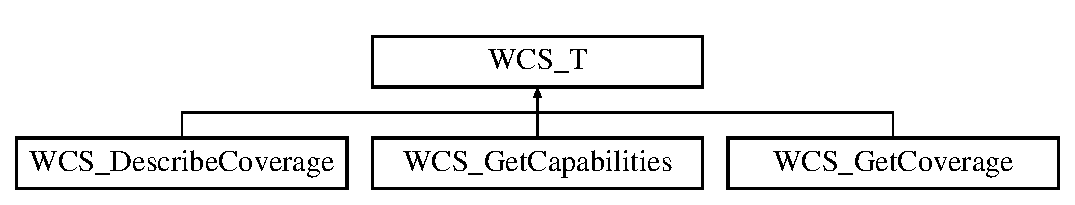
\includegraphics[height=2.000000cm]{classWCS__T}
\end{center}
\end{figure}
\subsection*{Public Member Functions}
\begin{DoxyCompactItemize}
\item 
\hyperlink{classWCS__T_a1bd0d238dffd912d223aa31709338f38}{WCS\_\-T} (const string \&conf)
\begin{DoxyCompactList}\small\item\em Constructor of a \hyperlink{classWCS__T}{WCS\_\-T} object. \end{DoxyCompactList}\item 
CPLErr \hyperlink{classWCS__T_a2edb33250f0cd0708e156197145d85ad}{InitializeConfigurationFiles} ()
\begin{DoxyCompactList}\small\item\em Initialize the configuration files and load the contents to memory. \end{DoxyCompactList}\item 
\hyperlink{classDatasetSeriesObject}{DatasetSeriesObject} \hyperlink{classWCS__T_ad100a5da6a0c7e7a95875ab19c2343a8}{InitializeDatasetSeriesByID} (string \&sCovID)
\begin{DoxyCompactList}\small\item\em Initialize the dataset series by specify the coverage identifier. \end{DoxyCompactList}\item 
\hyperlink{classDatasetObject}{DatasetObject} \hyperlink{classWCS__T_af4fe8b9d94363b4c9e3b6ce9f3097e1e}{InitializeDatasetByID} (string \&sCovID)
\begin{DoxyCompactList}\small\item\em Initialize the dataset by specify the coverage identifier. \end{DoxyCompactList}\item 
\hypertarget{classWCS__T_ab81521d2a98b5b0e9f438d26873655d5}{
void {\bfseries SetSoapMessage} (const int \&soapMsg)}
\label{classWCS__T_ab81521d2a98b5b0e9f438d26873655d5}

\item 
\hypertarget{classWCS__T_a558a55cd04ce9366d5412cf62731dd65}{
int {\bfseries IsSoapRequested} ()}
\label{classWCS__T_a558a55cd04ce9366d5412cf62731dd65}

\item 
void \hyperlink{classWCS__T_a9f29625a62a2a75cb9a258b8949e9496}{SendHttpHead} ()
\begin{DoxyCompactList}\small\item\em Sent the HTTP head type according to request type. \end{DoxyCompactList}\item 
\hypertarget{classWCS__T_a1476aba462b825963ac9330ba711038c}{
virtual CPLErr {\bfseries GetReqMessageFromXMLTree} (CPLXMLNode $\ast$xmlRoot)}
\label{classWCS__T_a1476aba462b825963ac9330ba711038c}

\item 
\hypertarget{classWCS__T_a1f65ae0e62b09d43416bedea82bc9ef1}{
virtual CPLErr {\bfseries GetReqMessageFromURLString} (const string \&)}
\label{classWCS__T_a1f65ae0e62b09d43416bedea82bc9ef1}

\item 
\hypertarget{classWCS__T_a7f7078f64c43d74cfa9c51eb4563f159}{
virtual void {\bfseries WCST\_\-Respond} (string \&sOutFileName)}
\label{classWCS__T_a7f7078f64c43d74cfa9c51eb4563f159}

\item 
\hypertarget{classWCS__T_a834314259a1babfcaf15f74c68ef1ab6}{
virtual void {\bfseries WCST\_\-Respond} ()}
\label{classWCS__T_a834314259a1babfcaf15f74c68ef1ab6}

\end{DoxyCompactItemize}
\subsection*{Public Attributes}
\begin{DoxyCompactItemize}
\item 
\hypertarget{classWCS__T_afffa45e7cce0bed7a0d99cab8d385531}{
int {\bfseries mb\_\-SoapRequest}}
\label{classWCS__T_afffa45e7cce0bed7a0d99cab8d385531}

\item 
\hypertarget{classWCS__T_a2090c46c1f538cdbf60c83f3bf5f7498}{
string {\bfseries ms\_\-Service\_\-op\_\-URL}}
\label{classWCS__T_a2090c46c1f538cdbf60c83f3bf5f7498}

\item 
\hypertarget{classWCS__T_a9b491a75bb8b8779ba83a16f2abda4e3}{
vector$<$ string $>$ {\bfseries mvs\_\-SupportFormats}}
\label{classWCS__T_a9b491a75bb8b8779ba83a16f2abda4e3}

\end{DoxyCompactItemize}
\subsection*{Protected Attributes}
\begin{DoxyCompactItemize}
\item 
\hypertarget{classWCS__T_a25a1dddf92f30d4ce4a0e7c3055c3efd}{
\hyperlink{classWCS__Configure}{WCS\_\-Configure} $\ast$ {\bfseries mp\_\-Conf}}
\label{classWCS__T_a25a1dddf92f30d4ce4a0e7c3055c3efd}

\item 
\hypertarget{classWCS__T_a83b82947270b9e75fa776ebff06cb5fd}{
vector$<$ \hyperlink{classDatasetObject}{DatasetObject} $>$ {\bfseries mv\_\-datasetCoverage}}
\label{classWCS__T_a83b82947270b9e75fa776ebff06cb5fd}

\item 
\hypertarget{classWCS__T_a268f2bb09efa55ab7cd328f8f79dd414}{
vector$<$ \hyperlink{classStitchedMosaicObject}{StitchedMosaicObject} $>$ {\bfseries mv\_\-stitchedMosaicCoverage}}
\label{classWCS__T_a268f2bb09efa55ab7cd328f8f79dd414}

\item 
\hypertarget{classWCS__T_a288a4d72e91b32e125e47407153ead98}{
vector$<$ \hyperlink{classDatasetSeriesObject}{DatasetSeriesObject} $>$ {\bfseries mv\_\-datasetSeriesCoverage}}
\label{classWCS__T_a288a4d72e91b32e125e47407153ead98}

\item 
\hypertarget{classWCS__T_abe41bcce822e58cd39bcbbeaebc865cf}{
string {\bfseries ms\_\-datasetConfPath}}
\label{classWCS__T_abe41bcce822e58cd39bcbbeaebc865cf}

\item 
\hypertarget{classWCS__T_a8f0b657e019f3ab00e7abb614b410bb8}{
string {\bfseries ms\_\-stitchedMosaicConfPath}}
\label{classWCS__T_a8f0b657e019f3ab00e7abb614b410bb8}

\item 
\hypertarget{classWCS__T_a7213d7699e60f0d54835c8a21bd80dc7}{
string {\bfseries ms\_\-datasetSeriesConfPath}}
\label{classWCS__T_a7213d7699e60f0d54835c8a21bd80dc7}

\item 
\hypertarget{classWCS__T_abcf3dec906024653cae1b00a2e2545a6}{
string {\bfseries ms\_\-iso19115Contents}}
\label{classWCS__T_abcf3dec906024653cae1b00a2e2545a6}

\item 
\hypertarget{classWCS__T_af971eb396be85676d54b62df318ad9a8}{
string {\bfseries ms\_\-eoMetadataContents}}
\label{classWCS__T_af971eb396be85676d54b62df318ad9a8}

\item 
\hypertarget{classWCS__T_a11312460f10652b429b21a1bb58fe442}{
string {\bfseries ms\_\-requestFullURL}}
\label{classWCS__T_a11312460f10652b429b21a1bb58fe442}

\end{DoxyCompactItemize}


\subsection{Detailed Description}
\hyperlink{classWCS__T}{WCS\_\-T} is a upper class for handling WCS request. 

This class is the upper class for handling WCS request. 

\subsection{Constructor \& Destructor Documentation}
\hypertarget{classWCS__T_a1bd0d238dffd912d223aa31709338f38}{
\index{WCS\_\-T@{WCS\_\-T}!WCS\_\-T@{WCS\_\-T}}
\index{WCS\_\-T@{WCS\_\-T}!WCS_T@{WCS\_\-T}}
\subsubsection[{WCS\_\-T}]{\setlength{\rightskip}{0pt plus 5cm}WCS\_\-T::WCS\_\-T (
\begin{DoxyParamCaption}
\item[{const string \&}]{conf}
\end{DoxyParamCaption}
)}}
\label{classWCS__T_a1bd0d238dffd912d223aa31709338f38}


Constructor of a \hyperlink{classWCS__T}{WCS\_\-T} object. 

This is the accepted method of creating an \hyperlink{classWCS__T}{WCS\_\-T} object. The path for served dataset, stitched mosaic and datasetSeries will be assigned to member variables through parsing configuration file. 

\subsection{Member Function Documentation}
\hypertarget{classWCS__T_a2edb33250f0cd0708e156197145d85ad}{
\index{WCS\_\-T@{WCS\_\-T}!InitializeConfigurationFiles@{InitializeConfigurationFiles}}
\index{InitializeConfigurationFiles@{InitializeConfigurationFiles}!WCS_T@{WCS\_\-T}}
\subsubsection[{InitializeConfigurationFiles}]{\setlength{\rightskip}{0pt plus 5cm}CPLErr WCS\_\-T::InitializeConfigurationFiles (
\begin{DoxyParamCaption}
{}
\end{DoxyParamCaption}
)}}
\label{classWCS__T_a2edb33250f0cd0708e156197145d85ad}


Initialize the configuration files and load the contents to memory. 

This method is used to parse configuration files for dataset/mosaci/datasetSeries coverage, and assign those information to corresponding array.

\begin{DoxyReturn}{Returns}
CE\_\-None on success or CE\_\-Failure on failure. 
\end{DoxyReturn}
\hypertarget{classWCS__T_af4fe8b9d94363b4c9e3b6ce9f3097e1e}{
\index{WCS\_\-T@{WCS\_\-T}!InitializeDatasetByID@{InitializeDatasetByID}}
\index{InitializeDatasetByID@{InitializeDatasetByID}!WCS_T@{WCS\_\-T}}
\subsubsection[{InitializeDatasetByID}]{\setlength{\rightskip}{0pt plus 5cm}{\bf DatasetObject} WCS\_\-T::InitializeDatasetByID (
\begin{DoxyParamCaption}
\item[{string \&}]{sCovID}
\end{DoxyParamCaption}
)}}
\label{classWCS__T_af4fe8b9d94363b4c9e3b6ce9f3097e1e}


Initialize the dataset by specify the coverage identifier. 

This method is used to initialize the dataset by specify the coverage identifier.


\begin{DoxyParams}{Parameters}
{\em sCovID} & Coverage indeifier.\\
\hline
\end{DoxyParams}
\begin{DoxyReturn}{Returns}
The corresponding Dataset object. 
\end{DoxyReturn}
\hypertarget{classWCS__T_ad100a5da6a0c7e7a95875ab19c2343a8}{
\index{WCS\_\-T@{WCS\_\-T}!InitializeDatasetSeriesByID@{InitializeDatasetSeriesByID}}
\index{InitializeDatasetSeriesByID@{InitializeDatasetSeriesByID}!WCS_T@{WCS\_\-T}}
\subsubsection[{InitializeDatasetSeriesByID}]{\setlength{\rightskip}{0pt plus 5cm}{\bf DatasetSeriesObject} WCS\_\-T::InitializeDatasetSeriesByID (
\begin{DoxyParamCaption}
\item[{string \&}]{sCovID}
\end{DoxyParamCaption}
)}}
\label{classWCS__T_ad100a5da6a0c7e7a95875ab19c2343a8}


Initialize the dataset series by specify the coverage identifier. 

This method is used to initialize the dataset series by specify the coverage identifier.


\begin{DoxyParams}{Parameters}
{\em sCovID} & Coverage indeifier.\\
\hline
\end{DoxyParams}
\begin{DoxyReturn}{Returns}
The corresponding DatasetSeries object. 
\end{DoxyReturn}
\hypertarget{classWCS__T_a9f29625a62a2a75cb9a258b8949e9496}{
\index{WCS\_\-T@{WCS\_\-T}!SendHttpHead@{SendHttpHead}}
\index{SendHttpHead@{SendHttpHead}!WCS_T@{WCS\_\-T}}
\subsubsection[{SendHttpHead}]{\setlength{\rightskip}{0pt plus 5cm}void WCS\_\-T::SendHttpHead (
\begin{DoxyParamCaption}
{}
\end{DoxyParamCaption}
)}}
\label{classWCS__T_a9f29625a62a2a75cb9a258b8949e9496}


Sent the HTTP head type according to request type. 

This method is used to send the HTTP head type according to request type. As to SOAP request: 
\begin{DoxyCode}
 Content-Type: application/xml+soap
\end{DoxyCode}


As to POST request: 
\begin{DoxyCode}
 Content-Type: text/xml
\end{DoxyCode}
 

The documentation for this class was generated from the following files:\begin{DoxyCompactItemize}
\item 
WCS\_\-T.h\item 
WCS\_\-T.cpp\end{DoxyCompactItemize}

\hypertarget{classWCSCGI}{
\section{WCSCGI Class Reference}
\label{classWCSCGI}\index{WCSCGI@{WCSCGI}}
}


{\ttfamily \#include \char`\"{}wcsUtil.h\char`\"{}}

\subsection*{Public Member Functions}
\begin{DoxyCompactItemize}
\item 
CPLErr \hyperlink{classWCSCGI_a63c7630dd9f2df7186b533552f898f04}{Run} ()
\begin{DoxyCompactList}\small\item\em The entry point for CGI program. \end{DoxyCompactList}\item 
\hypertarget{classWCSCGI_aa680e2c779778dc6bd8b974735d1debc}{
string {\bfseries GetRqstContent} ()}
\label{classWCSCGI_aa680e2c779778dc6bd8b974735d1debc}

\item 
\hypertarget{classWCSCGI_aa995556ffcea2aa59059b9112c4b11ef}{
CGI\_\-METHOD\_\-FLAG {\bfseries GetCGImethod} ()}
\label{classWCSCGI_aa995556ffcea2aa59059b9112c4b11ef}

\end{DoxyCompactItemize}


\subsection{Detailed Description}
\hyperlink{classWCSCGI}{WCSCGI} class is used to acquire WCS request, both GET and POST method are supported. 

\subsection{Member Function Documentation}
\hypertarget{classWCSCGI_a63c7630dd9f2df7186b533552f898f04}{
\index{WCSCGI@{WCSCGI}!Run@{Run}}
\index{Run@{Run}!WCSCGI@{WCSCGI}}
\subsubsection[{Run}]{\setlength{\rightskip}{0pt plus 5cm}CPLErr WCSCGI::Run (
\begin{DoxyParamCaption}
{}
\end{DoxyParamCaption}
)}}
\label{classWCSCGI_a63c7630dd9f2df7186b533552f898f04}


The entry point for CGI program. 

This method is used to fetch CGI parameters. Supports both HTTP GET and POST method. POST content could be KVPs and XML string, and GET content must be KVPs.

\begin{DoxyReturn}{Returns}
CE\_\-None on success or CE\_\-Failure on failure. 
\end{DoxyReturn}


The documentation for this class was generated from the following files:\begin{DoxyCompactItemize}
\item 
wcsUtil.h\item 
wcsUtil.cpp\end{DoxyCompactItemize}

\printindex
\end{document}
